\documentclass[10pt,spanish]{book}
\usepackage{graphicx,babel}
\usepackage{epstopdf}
\usepackage{newcent}
\usepackage{tabularx}
\usepackage{amssymb}
\usepackage{epic}
\usepackage{palatino}
%\usepackage{bookman}
%\usepackage{times}
\usepackage[T1]{fontenc}    % Usar la codificaci�n T1
\usepackage{graphics}
\usepackage{tabularx,supertabular}
\usepackage{fancyhdr}
\usepackage{makeidx}
\usepackage[version=3]{mhchem}
\usepackage[refpages]{gloss}

%\DeclareGraphicsRule{.tif}{png}{.png}{`convert #1 `dirname #1`/`basename #1 .tif`.png}
\newcommand{\HRule}{\rule{\linewidth}{1mm}}
\setlength{\parindent}{0mm}
\setlength{\parskip}{0mm}
\newcounter{nejemplo}
%
  \makeatletter
%   \newcommand\reaction@[2]{\begin{equation}\ce{#1} \label{#2} \end{equation}}
    \newcommand\reaction@[1]{\begin{equation}\ce{#1}\end{equation}}
    \newcommand\reaction@nonumber[1]%
      {\begin{equation*}\ce{#1}\end{equation*}}
    \newcommand\reaction{\@ifstar{\reaction@nonumber}{\reaction@}}
  \makeatother
%
\newcommand{\ejemplo}[2]{%
\stepcounter{nejemplo}
\medskip
\tablefirsthead{ \hline {\bf Ejemplo \arabic{chapter}.\arabic{section}.\arabic{nejemplo} #1}\\\hline}
%\tablehead{ \hline {\small \slshape Ejemplo \arabic{chapter}.\arabic{section}.\arabic{nejemplo} continuaci\'on\ }\\\hline}
%\tabletail{\hline\small\slshape continua\hline}
\tablelasttail{\hline}%
\begin{supertabular}%
{|p{0.97\textwidth} |}%
 \small #2\\ %
 \end{supertabular}\smallskip }%

\selectspanish
\decimalpoint
\makeindex
\makegloss

\setglossgroup{C}{Signos}
\setglossgroup{S}{S\'{\i}mbolos}

%\listfiles
\begin{document}

\newcounter{cm}
\setlength{\unitlength}{1mm}
\newcolumntype{Y}{>{\centering\arraybackslash}X}%

\pagestyle{fancy}
\addtolength{\headwidth}{.8\marginparwidth}
\renewcommand{\chaptermark}[1]{\markboth{#1}{}}
\renewcommand{\sectionmark}[1]{\markright{\thesection\ #1}}
\fancyhf{} 
\fancyhead[LE,RO]{\bfseries\thepage}
\fancyhead[LO]{\bfseries\rightmark}
\fancyhead[RE]{\bfseries\leftmark}
\renewcommand{\headrulewidth}{0.5pt}
\renewcommand{\footrulewidth}{0pt}
\addtolength{\headheight}{2.0pt}
\fancypagestyle{plain}{
    \fancyhead{}
    \renewcommand{\headrulewidth}{0pt}
}

{\pagestyle{empty}
\bibliographystyle{acm}
\frontmatter
\title{\HRule\\[5mm]\Huge Fisicoqu\'{\i}mica B\'asica Atmosf\'erica }
\author{Dr. Jos\'e Agust\'{\i}n Garc\'{\i}a Reynoso \\
M.C. Alejandra Mendoza Campos\\[1mm] \HRule}
\date{\textsc{ 25 de agosto del 2010}}
\maketitle

\pagestyle{fancy}
\setcounter{page}{1}
\tableofcontents
\listoftables
\listoffigures
   }
{\mainmatter

\pagestyle{fancy}
\chapter*{Introducci\'on}

Dentro del posgrado en Ciencias de la Tierra se recibe una gran diversidad de estudiantes que provienen de diferentes \'areas del conocimiento. Si bien muchos de ellos estudiaron y revisaron durante el bachillerato parte de los temas que aqu\'{\i} se presentan, \'estos no son revisados dentro de sus respectivas carreras profesionales. El motivo de este trabajo es ayudar  a recordar y a presentar los temas relacionados a la fisico qu\'{\i}mica atmosf\'erica. que sean \'utiles para el desarrollo de sus estudios en lel posgrado.

 En la primera parte se presentan los temas fundamentales de la termodin\'a mica, con base en las leyes de la termodin\'a mica, energ\'{\i}a libre, reacciones en los seres vivos. Posteriormente se abordan los temas de procesos electroqu\'{\i}micos donde se ven los fen\'omenos de \'oxido-reducci\'on, los sistemas electroqu\'{\i}micos y la corrosi\'on.
 
 Si bien la termodin\'amica nos indica la espontaneidad de un proceso, lo anterior no nos indica la rapidez con la que se puede dar, por lo que se abordan los temas de cin\'etica qu\'{\i}mica, teor\'{\i}a de colisiones, energ\'{\i}a de activaci\'on  y los factores que influyen en la rapidez de una reacci\'on.
 
 En la parte de equilibrio qu\'{\i}mico se aborda el tema reversibilidad de las reacciones, la constante de equilibrio y algunas aplicaciones de la misma con el $p$H.
 
 En la parte de qu\'{\i}mica org\'anica se hace una descripci\'on de los niveles de energ\'{\i}a en los \'atomos, las cofiguraciones electr\'onicas, los s\'{\i}mbolos de Lewis, lo que es la energ\'{\i}a de ionizaci\'on. Se muestran las familias de compuestos org\'anicos basados en el n\'umero de enlaces entre \'atomos de carbono y con otros elementos como el ox\'{\i}geo y el nitr\'ogeno.
 
 En la segunda parte se muestran los compuestos considerados como contaminantes y su clasificaci\'on, el manejo de unidades de los mismos y los procesos fisicoquimos  en la atm\'esfera en los que \'estos intervienen.
 
 Si el lector desea profundizar en  algún tema se presenta la bibliograf\'{\i}a complementaria a los temas tratados.
 
 Se espera que sea un libro texto para aquellos quienes los temas de qu\'{\i}mica son poco estudiados dentro de sus formaci\'on profesional.
 
 
\part{Teor\'{\i}a}
\chapter[Energia y reacciones]{La energ\'{\i}a y las reacciones qu\'{\i}micas}

El estudio de la energía y las reacciones químicas es fundamental para comprender los procesos que rigen tanto la naturaleza como las aplicaciones tecnológicas. Este capítulo explora los principios básicos de la termodinámica, la electroquímica y la termoquímica, proporcionando una base sólida para entender cómo la energía se transforma y se transfiere en los sistemas químicos.

En la \textbf{Sección 1.1}, se introduce el concepto de \textbf{energía} y su relación con las reacciones químicas. Esta parte se inicia con el desarrollo de la noción de sistema, estados y funciones de estado. Se analizan los tipos de sistemas, las propiedades de un sistema y los cambios de estado, junto con el comportamiento de los gases ideales y no ideales, las ecuaciones de estado y la Ley General de los Gases. Además, se interpreta el significado de la primera ley de la termodinámica, expresada como $\Delta E = q + w$, que establece la conservación de la energía. Se establece la diferencia entre energía interna y entalpía, y se clasifican las reacciones en exotérmicas y endotérmicas.

En la \textbf{Sección 1.2}, se estudia la forma en que se presentan gráficamente los cambios de energía asociados a los cambios químicos, así como la relación entre las entalpías de reacción y las energías de enlace. Se definen los estados estándares y se explica cómo las entalpías de formación y la Ley de Hess se aplican en cálculos termoquímicos. Estos conceptos permiten comprender y predecir los cambios energéticos en reacciones químicas complejas.

En la \textbf{Sección 1.3}, se introduce el concepto de \textbf{entropía} ($\Delta S$), una medida del desorden en un sistema, y su relación con los cambios de energía en transformaciones físicas y químicas. Se interpreta y aplica la ecuación que relaciona energía libre, entalpía y entropía: $\Delta G = \Delta H - T \Delta S$. Se analiza la importancia de la variación de la energía libre durante un cambio químico como criterio para predecir, sin necesidad de experimentos, si un proceso puede ocurrir o no. Finalmente, se estudia la relación entre la energía libre, los procesos espontáneos y las reacciones exergónicas y endergónicas.

La \textbf{Sección 1.4} aborda los \textbf{procesos electroquímicos}, incluyendo las reacciones de oxidación-reducción, las celdas electroquímicas (galvánicas y electrolíticas), los sistemas electroquímicos y el potencial estándar de reducción. También se discuten temas relacionados con la corrosión de metales y las estrategias para su prevención.

Este capítulo proporciona una visión integral de los principios energéticos y químicos que rigen los procesos naturales y tecnológicos, sentando las bases para su aplicación en diversos campos de la ciencia y la ingeniería.

\section{Sistemas, estados y funciones de estado}
\index{sistema}
 Un \textit{\gloss[word]{sistema} termodin\'a\-mi\-co} es una porci\'on del universo separada por fronteras que nos interesa estudiar, tambi\'en se puede definir como la parte del universo f\'{\i}sico cuyas propiedades se est\'an investigando. El sistema est\'a confinado a un lugar definido en el espacio por la \gloss[word]{frontera}\index{sistema!frontera} que lo separa del resto del universo (el medio exterior). La ciencia que estudia c\'omo la energ\'{\i}a y propiedades mesurables de un sistema se relacionan y la interacci\'on con los alrededores es la \textbf{\gloss[word]{termodinamica}} \index{termodinamica@termodin\'amica} su nombre procede del griego \textit{termos} (calor) y \textit{dinamos} (movimiento). Es parte de la f\'{\i}sica que trata del estudio de los procesos en los que se transfiere energ\'{\i}a o sus manifestaciones como calor y como trabajo. 

\subsection{Tipos de sistemas}

\index{sistema!tipos}
\begin{itemize}
\item \textit{Aislado} cuando la frontera evita cualquier interacci\'on con la materia o  energ\'{\i}a del exterior.
\item \textit{Abierto} cuando pasa materia a trav\'es de la frontera.
\item \textit{Cerrado} aquel que no intercambia materia con sus alrededores pero s\'{\i} ener\-g\'{\i}a.
\item \textit{Homog\'eneo} cuando contiene \'unicamente una fase.
\item \textit{Heterog\'eneo} contiene m\'as de una fase.
\end{itemize}

Se define a una \gloss[word]{fase}\index{sistema!fase} como una porci\'on homog\'enea del sistema, f\'{\i}sica\-mente diferenciable y separable mec\'anicamente. Si el sistema ``agua'' coexisten las tres formas s\'olida (hielo), l\'{\i}quida y gaseosa (vapor), cada una constituye una fase separada de las otras por un l\'{\i}mite.


\subsection{Propiedades de un sistema}
Las propiedades de un sistema\index{sistema!propiedades} son los atributos f\'{\i}sicos que perciben los sentidos directamente o con un m\'etodo experimental. La presi\'on y el vo\-lumen son propiedades f\'acilmente perceptibles a las que se les designa un valor num\'erico. La entalp\'{\i}a es una propiedad que s\'olo se detecta con un experimento y no se mide su valor absoluto sino sus cambios.

Las propiedades del sistema se dividen en dos clases:

\begin{itemize}
\item \textit{Intensivas} \index{propiedades!intensivas} son aquellas que no dependen de la cantidad de substancia o del tama\~no de un sistema, por lo que el valor permanece inalterable al subdividir el sistema inicial en varios subsistemas. Entre estas propiedades se encuentra la densidad (\gloss[word]{densidad}), el \'{\i}ndice de refracci\'on, la masa molar, el volumen molar y la e\-nerg\'{\i}a molar. 
\item \textit{Extensivas} \index{propiedades!extensivas}son aquellas que si dependen de la cantidad de sustancia o del tama\~no de un sistema, son magnitudes cuyo valor es proporcional al tama\~no del sistema que describe, dependen de dos de las tres variables presi\'on ($P$), volumen ($V$) y temperatura ($T$) y el n\'umero de moles.
\end{itemize}

\subsection{Estado de un sistema}
\index{sistema!estado}
Un sistema se encuentra en un estado definido cuando cada una de sus propiedades tiene un valor determinado. Debemos saber que con base en el estudio experimental del sistema o de la experiencia con sistemas semejantes, qu\'e propiedades deben considerarse, con el fin de que el estado del sistema sea definido con precisi\'on suficiente para el prop\'osito buscado.

\begin{example}[Estado de un sistema]El estado est\'andar del agua l\'{\i}quida a $25\celsius$ y 1 \bbar \footnote{ La IUPAQ con base en el trabajo del Comit\'e de Datos para la ciencia y Tecnolog\'{\i}a (CODATA) recientemente recomend\'o que el estado est\'andar se refiera a la presi\'on de 1 \bbar (100 000\pascal). La diferencia entre una atm\'osfera y un bar es de alrededor de 1\% .}.
\end{example}

 El estado est\'andar se describe con un cero como super\'{\i}ndice, por ejemplo $\Delta H^\circ$. Este s\'{\i}mbolo expresa en los textos que siguen la convenci\'on antigua, que los valores corresponden a  la presi\'on de 1 atm\'osfera.

\subsection{Cambio de estado, trayectoria, ciclo, proceso}

Sometamos a un sistema a un cambio de estado \index{sistema!cambio de estado} desde
condiciones espec\'{\i}ficas iniciales hasta condiciones espec\'{\i}ficas finales.

El \textit{cambio de estado}\index{estado!cambio} est\'a completamente  definido cuando se especifica el estado inicial y el estado final.

La \textit{trayectoria} \index{estado!trayectoria} del cambio de estado se define especificando el estado inicial, la secuencia de estados intermedios que va tomando el sistema y el estado final.

Un \textit{proceso} \index{proceso} es el m\'etodo de operaci\'on mediante el cual se realiza un cambio de estado. La descripci\'on de un proceso consiste en establecer todo o parte de los siguientes: (1) la frontera; (2) cambio de estado, la trayectoria o los efectos producidos en el sistema durante cada etapa del proceso y (3) los efectos producidos en el medio externo durante cada etapa del proceso.

Supongamos que un sistema sometido a un cambio de estado regrese a su estado inicial. La trayectoria de esta transformaci\'on c\'{\i}clica se llama ciclo y el proceso mediante el cual se realiz\'o la transformaci\'on se llama \textit{proceso c\'{\i}clico}.

Una \textit{\gloss[word]{variabledeestado}} \index{estado!variable} es aquella que tiene un
valor definido cuando especifica el estado de un sistema.

En la siguiente parte se mostrar\'an los conceptos para poder responderse a preguntas tales como: ?`Qu\'e es un sistema?, ?`D\'onde existe una frontera?, ?`Cu\'al es el estado inicial?, ?`Cu\'al es el estado final?, ?`Cu\'al es la trayectoria de transformaci\'on?.


\subsection{Gases ideales} 
Los \gloss[word]{gasesideales}\index{gases ideales} son aquellos cuyo comportamiento no se
altera por fuerzas de cohesi\'on y vol\'umenes moleculares. Los \gloss[word]{gasesreales}
est\'an m\'as cercanos al comportamiento ideal mientras m\'as bajas sean las
presiones y m\'as altas las temperaturas.

\subsection{Ecuaciones de estado}

Las ecuaciones\index{estado!ecuaciones}  que representan las relaciones presi\'on
(\gloss[Word]{presion})- volumen (\gloss[Word]{volumen}) -
temperatura(\gloss[Word]{temperatura}) de los gases se conocen como \gloss[word]{ecuaciondeestado}, ya que describen completamente el estado de cualquier
sistema gaseoso. Las variables de estas ecuaciones se dividen en dos clases:
moles (\gloss[word]{moles}) y $V$ son variables extensivas (propiedades que dependen de la
cantidad de material) mientras que $P$ y $T$ son intensivas.

\begin{figure}[h]

\begin{center}
\begin{tabular}{||c|c|c|c|c|c||} \hline \hline
      &           &          &           &  & \\ \hline
      &           &          &           &  & \\ \hline
      &           &          &           &  & \\ \hline
      &           &          &           &  & \\ \hline
      &           &          &           &  &  \\ \hline \hline
\end{tabular}
\caption{Subdivisi\'on del sistema}
\label{fig:1}
\end{center}
\end{figure}


El valor de cualquier propiedad extensiva\index{estado!propiedad extensiva} se obtiene sumando
los va\-lores de la misma en todas partes del sistema. Supongamos que el sistema est\'a
subdividido en muchas partes peque\~nas, como en la Figura~\ref{fig:1}, entonces el volumen total del sistema se obtiene sumando los vol\'umenes de
cada una de las partes.

Las propiedades intensivas\index{estado!propiedad intensiva} no se obtienen mediante tal
proceso de su\-ma, sino que se miden de cualquier punto del sistema y cada una tiene un valor
uniforme en cualquier punto del sistema en equilibrio; por ejemplo, $T$ y $P$.

La temperatura ($T$) en todas las ecuaciones de estado es la \index{temperatura!absoluta} \gloss[word]{temperaturaabsoluta} es decir para el sistema m\'etrico decimal se encuentra en Kelvin\footnote{ Es importante identificar que la abreviatura $\kelvin$ de Kelvin es en may\'uscula mientras que de kilo (k) es en min\'uscula. As\'{\i} Kg representa Kelvin gramo y $\kilogram$ es kilogramo.} .

\begin{equation}
T[K]_{absoluta} = T[\degreecelsius] + 273.15
\end{equation}

\textit{Ley de \gloss[Word]{boyle}} \index{Boyle@\textbf{Boyle}!Ley de} Siempre que la masa
y la temperatura de una muestra de gas se mantienen constantes, el volumen del gas es
inversamente proporcional a su presi\'on absoluta.
\begin{equation}
P \propto \frac{1}{V} \quad{ \longrightarrow }\quad  P = \frac{k}{V}
\end{equation}
Tambi\'en podemos escribirla de la siguiente manera:
\begin{equation}
P_1 V_1 = P_2 V_2
\end{equation}
\begin{example}[Ley de Boyle]
 Un gas se comprime isotermicamente de $P_1= 1 \bbar$  y  $V= 10 \liter$  a una presi\'on de 2 \bbar. ?`Cu\'al es su volumen?\\[3pt]

$V_2 = \frac{P_1 V_1}{P_2}$\hskip.3in substituyendo\hskip.3in  $V_2 = \frac{1\bbar(10\liter)}{2 \bbar} = 5 \liter$
\end{example}

\textit{Ley de \gloss[Word]{charles}}\index{Charles@\textbf{Charles}} Siempre que la masa y la presi\'on de una muestra de gas se mantienen constantes, el volumen de la muestra es directamente proporcional a su temperatura absoluta.
\begin{equation}
V= k'T
\end{equation}
que tambi\'en se puede escribir de la siguiente forma:
\begin{equation}
\frac{V_1}{T_1} = \frac{V_2}{T_2}
\end{equation}

\begin{example} [Ley de Charles]
 A un gas ideal se le incrementa la temperatura a presi\'on constante de T = 15$\degreecelsius$ a 125 $\degreecelsius$ si su volumen
inicial es de 100 L. ?`Cu\'al es su volumen final?. \vskip0.1in
Para convertir la temperatura a absoluta se suman 273.15 $\kelvin$ as\'{\i} tenemos que 15$\degreecelsius$ son 288.15 y 125$\degreecelsius$ 398.15\kelvin
\vskip.2in
${V_2} = \frac{V_1 \times T_2}{T_1}$\hskip.25in sustituyendo\hskip.25in 
$V_2 = \frac{100\liter \times 398.15 \kelvin}{288.15 \kelvin} = 138.17 \liter$
\end{example}\vskip0.1in

\textit{Ley combinada de los gases} \index{ley combinada de los gases}. Empleando las ecuaciones anteriores se puede obtener la siguiente realci\'on entre el volumen, presi\'on y temperatura:
\begin{equation}
\frac{P_1V_1}{T_1} = \frac{P_2V_2}{T_2}
\end{equation}

 
 \subsection{Ley General de los gases}
 \index{ley!general de los gases}
 La ley general de los gases se puede aplicar para las condiciones de presi\'on y temperatura ambiente. La relaci\'on que guarda la temperatura, presi\'on, volumen y cantidad de masa se muestra en la siguiente ecuaci\'on:

\begin{equation}
PV = nRT\label{lgg}
\end{equation}

donde :

\qquad\begin{tabular}{c@{ -- }ll}
$P$ & presi\'on &[atm]\\
$V$ & volumen &[L]\\
$n$ & moles de gas &[\gram\mole]\\
\gloss[Word]{constR}& Constante de los gases&[\litre-atm/(\gram\mole \kelvin)]  \index{constante!ley general de los gases}\\
$T$ & temperatura absoluta&[\kelvin]\\
\end{tabular}

\begin{example}
?`Cu\'al es el volumen que ocupan 112 g de Nitr\'ogeno (N$_2$) a la presi\'on de la Ciudad de M\'exico (0.77 atm) y a una temperatura de $15 \degreecelsius$. (R = 0.082057 $\frac{\textrm{L-atm}}{\textrm{gmol} \kelvin}$)%


Convirtiendo los 15$\degreecelsius$ a absoluta tenemos 288.15\kelvin

Moles de N$_2$ = $\frac{112 \gram}{28 \frac{\gram}{\textrm{gmol}}} =$ 4 \gram\mole

$V = \frac{nRT}{P}$\hskip.10in substituyendo  \hskip.10in $V = \frac{4
\gram\mole \times 0.082057 \frac{\liter-\mathrm{atm}}{\gram\mole\, \kelvin} \times 288 \kelvin} {0.77 \mathrm{atm}}$\vskip0.1in

$V = 122.7$ \liter
\end{example}

y a partir de la \textbf{Ec.~\ref{lgg}} se puede despejar los t\'erminos para calcular la densidad de un gas mediante la siguiente ecuaci\'on :
\index{densidad!c\'alculo}
\begin{equation}
\rho = \frac{PM}{RT}
\label{ecdensidad}
\end{equation}

\begin{tabular}{llll}
Donde:\\
&\gloss[word]{densidad} & Densidad del gas & [$\frac{\kilo\gram}{\cubic\metre}$]\\
&$P$ & Presi\'on   &[atm]\\
&$M$ & Peso molecular del gas&[g/gmol]\\
&$R$ & Constante de los gases& [$\frac{\liter-\textrm{atm}}{\gram\mole\; \kelvin}$] \\
&$T$ & Temperatura  &[\kelvin] \\
\end{tabular}

\begin{example}[Ley general de los gases]%
 Calcular la densidad de un gas cuyo peso molecular es 29.98 g/gmol, a una presi\'on de
0.8 atm\'osferas y a una temperatura de 130\degreecelsius.\\
\begin{enumerate}
\item Calcular la temperatura en Kelvin.

 Si T[K] = T[\degreecelsius] $+ 273.15$ entonces  T[\kelvin] $= 130 +273.15 = 403.15$
\item Empleando la ecuaci\'on~\ref{ecdensidad} tenemos:

$\rho=\frac{PM}{RT}
=\frac{0.8(29.98)}{0.082057(303.15)} = 0.725\frac{\kilo\gram}{\cubic\metre} = 0.0452\frac{\mathrm{lb}}{\mathrm{ft}^3}$
\end{enumerate}
\end{example}

\subsection{Unidades empleadas en concentraciones atmosféricas}
 \index{unidades}
Los resultados de las mediciones de compuestos traza en el aire  realizadas para su estudio, evaluaci\'on y control se expresan en diferentes unidades, provenientes de distintos campos de estudio. En esta parte se presentan las unidades empleadas y sus diferentes factores de conversi\'on.

\vskip .15in
\begin{tabularx}{.9\linewidth}{XXXX}
\textbf{Longitud}&&\textbf{\'Area}\\
 1 pie (ft)& 0.3048 m& 1 pie (ft)$^2$ & 0.0929 m$^2$\\
 1 pie (ft)& 12 pulgada (in)\\
 1 pulgada (in)  & 2.54 cm\\
\textbf{Volumen}&&\textbf{Presi\'on}\\
1 pie$^3$ (ft$^3$)& 0.028317 m$^3$ &1 atm & 14.69 psi\\ 
1 pie$^3$ (ft$^3$)& 1728 in$^3$    &1 atm & 760 mmHg \\
1 pie$^3$ (ft$^3$)& 7.481 gal      &1 atm & 101,325 pa\\
\textbf{Masa}    &         &1 ``C.A. & 2.4908 pa\\
 1 lb& 7,000 gr            &1 ``C.A. & 0.03614 psi\\
 1 lb& 0.454 kg            &1 ``C.A. & 0.57818 onzas/in$^2$\\
\end{tabularx}

\begin{tabularx}{.9\linewidth}{XXXX}
\textbf{Constante }&\textbf{de los gases}&\textbf{Densidad}\\
0.082057 $\frac{\liter-\mathrm{atm}}{\gram\mole\, \kelvin}$&10.73
$\frac{\mathrm{lb}}{\mathrm{in}^2}\frac{\mathrm{pie}^3}{\mathrm{lbmol R}} $&1 $\frac{\mathrm{lb}}{\mathrm{pie}^3}$& 16.02
$\frac{\kilo\gram}{\metre^3}$\\\end{tabularx}
\index{constante!ley general de los gases}


Las conversiones entre diferentes unidades de concentraci\'on son las siguientes:

\begin{tabular}{lrl}
Multiplicar&por&para obtener\\\hline
1 ppm$_v$   &1 & \micro\mole\, de gas/\mole\, de gas\\
&1 $\times10^{-4}$ & porcentaje en volumen (\%$_v$)\\
&$\frac{\textrm{{\footnotesize Peso Molecular}}}{24.45}$&\milli\gram/\cubic\metre de aire\\
&&a (25\celsius\; y 1 atm )\\
&1 $\times10^{-6}$ &$\frac{\textrm{Presi\'on parcial de un
constituyente}}{\textrm{Presi\'on total de la mezcla}}$\\
ppb$_v$& 1 $\times10^{-3}$ & Partes por mill\'on (ppm)\\
1 \%$_v$&10 000&Partes por mill\'on (ppm)\\
mg/l &1 000&{\small miligramos sobre metro c\'ubico (mg/\cubic\metre)}\\
$\mu$g/m$^3$ & 1$\times 10^{-6}$ &miligramos sobre
litro (mg/\liter)\\\hline
\end{tabular}\index{concentraci\'on!unidades}
\vskip.1in
Para convertir concentraciones de gases y vapores de partes por mill\'on en volumen a miligramos por metro c\'ubico y viceversa a cualquier temperatura y presi\'on, se pueden emplear las siguientes ecuaciones:\index{concentraci\'on!conversiones}
\begin{eqnarray*}
\textrm{Concentraci\'on,}\; \textrm{ppm}&=&\frac{C_1\times24.45 \times
T}{{\textrm M}\times298\times P}\\
\textrm{Concentraci\'on,}\;\milli\gram/\cubic\metre&=& \frac{C_2\times {\textrm
M}\times298\times P}{24.45\times T}
\end{eqnarray*}
\begin{tabular}{llll}
Donde:\\
&$C_1$ & Concentraci\'on del gas & [\milli\gram/\cubic\metre]\\
&$C_2$ & Concentraci\'on del gas & [ppm$_v$]\\
&$T$ & Temperatura&[\kelvin]\\
&$M$ & Peso Molecular del gas&[\gram/\gram\mole]\\
&$P$ & Presi\'on&[atm]\\
\end{tabular} 
 
\subsection{Peso molecular promedio}
\index{peso molecular promedio}
El peso molecular promedio  ($\overline{\textrm{M}}$) , \'este se obtiene de sumar los valores obtenidos de multiplicar la fracci\'on mol ($y_i$) de cada compuesto con su respectivo peso molecular ($\textrm{M}_i$),
\begin{equation}
\overline{\textrm{M}}=\sum_{i=1}^ny_i\textrm{M}_i
\label{peso1}
\end{equation}

La fracci\'on mol ($y_i$)\index{fracci\'on mol} se puede obtener a partir del por ciento en volumen (\%$_v$) del gas en la mezcla de la siguiente forma:

\begin{equation}
y_i = \frac{\%_{vi} }{100} 
\label{fraccion}
\end{equation}

También se puede obtener la fracción molar de cada componente  como:

\begin{equation}
y_i = \frac{n_i}{\sum n_i}
\end{equation}

donde $n_i$ es el número de moles del gas $i$ en la mezcla.

Com\'unmente el an\'alisis de los gases se obtiene sin considerar la humedad del aire por lo cual se calcula el peso molecular promedio en base seca ($\overline{\textrm{M}}_s$) y a partir de conocer el porcentaje de humedad (\%H) en la mezcla se puede calcular el peso molecular base h\'umeda ($\overline{\textrm{M}}_w$). Mediante la siguiente relaci\'on:
\index{peso molecular promedio!base seca}
\index{peso molecular promedio!base h\'umeda}
\begin{equation}
\overline{\textrm{M}}_w= \frac{\%H}{100}\times \textrm{M}_{H_2O} +
\frac{100-\%H}{100} \times \overline{\textrm{M}}_s
\label{hum}
\end{equation}
Este cálculo es esencial en aplicaciones como la química atmosférica, la ingeniería de procesos y la termodinámica de gases, donde se requiere conocer el comportamiento global de una mezcla gaseosa en función de sus propiedades individuales. 

Además, el peso molecular promedio es un factor clave en la determinación de propiedades como la densidad de la mezcla, la velocidad de difusión de los componentes y la viscosidad del gas. En el estudio de la atmósfera, este valor permite comprender la variabilidad de la composición del aire en diferentes condiciones ambientales y su impacto en los procesos de transporte y reacción química en la troposfera y estratosfera.

\subsubsection{N\'umero de Avogadro (N$_A$)}
 \index{Avogadro!numero@n\'umero}
 
 El n\'umero de Avogadro representa el n\'umero de mol\'e\-culas o \'atomos en una mol de cualquier compuesto o elemento. Su valor es de 6.022$\times10^{23}$moleculas/mol.
 
\begin{example}[N\'umero de mol\'eculas de \ce{CO2}]%
 El \ce{CO2} ocupa alrededor de 354 ppm$_v$ de aire. ?`Cu\'antas mol\'eculas de \ce{CO2} hay en 1m$^3$ de aire a 1 atm y 0\celsius?\\
 A partir de $PV =nRT$  obtenemos $\frac{n}{V}=\frac{P}{RT}\cdot N_A=2.69\times10^{25} \frac{\textrm{molec}}{\cubic\metre}$\\
 Sabemos que$ \frac{\ce{Vol CO2}}{\ce{Vol Aire}}=\frac{\ce{Molec CO2}}{\ce{Molec Aire}}$ entonces:\\
\quad $\frac{354 \milli\liter}{\liter \cubic\metre}=\frac{3.54\times10^{-6}\cubic\metre}{1m^3}=\frac{\# molec \ce{CO2}}{2.69\times10^{25}}$\\
\quad n\'umero de moleculas de \ce{CO2}

$=3.54\times10^{-6}\cubic\metre\times2.69\times10^{25}\frac{\textrm{molec}}{\cubic\metre} =9.52\times10^{21}\textrm{molec}$\\
\end{example}
 
\subsubsection{Constante de Boltzman}
\index{Boltzman!constante}
Es la constante de los gases para N$_A$ mol\'eculas.

\[
\begin{array}{rcl}
k  &=&\frac{R}{N_A}  \\
k  &=&\frac{0.082057\frac{\litre-\mathrm{atm}}{\mole-\kelvin}}{6.022\times10^{23}}   \\    
k  &=&1.362\times10^{-25}\frac{\litre-\mathrm{atm}}{\mathrm{molecula}\: \kelvin}
\end{array}
\]

\begin{example}[Peso Molecular  Promedio]%
\index{peso molecular promedio!ejemplo}%
Calcular el peso molecular promedio del un flujo de gas de un proceso de calcinaci\'on\footnote{Proceso de calentar una sustancia a temperatura elevada, pero por debajo de su punto de fusi\'on.} que tiene la siguiente composici\'on: 15\% ox\'{\i}geno (\ce{O2}), 8\% bi\'oxido de carbono (\ce{CO2}),  69.55\% de nitr\'ogeno (N$_2$) y 7.45\% de agua (\ce{H2O}).\\
Aplicando las ecuaciones \ref{peso1} y \ref{fraccion} se genera la siguiente tabla donde se obtiene el peso molecular promedio $\overline{\textrm{M}}$\footnote{\%$_v$ --- es el por ciento en volumen del compuesto en el gas\\
$y_i$ --- es la fracci\'on volumen o mol del compuesto $i$ en la mezcla gaseosa\\
 M$_i$ --- es el peso molecular del compuesto $i$ \\
 $y_i\times M_i$ --- es la fracci\'on de peso molecular del compuesto $i$ en la mezcla gaseosa.} 
\begin{footnotesize}

\begin{tabular}{c r@{.}l r l r@{.}l}
Compuesto& \multicolumn{2}{c}{\%$v$ } &$y$ & M$_i$&\multicolumn{2}{c}{$y\times M$}\\\hline 
\ce{O2}    &   15&0  &0.150& 32   & 4&800\\
\ce{CO2}   &    8&0  &0.080& 44   & 3&520\\
\ce{N2}    &   69&55 &0.695& 28   &19&474\\
\ce{H2O}   &    7&45 &0.075& 18   & 1&341\\ \hline
 $\overline{\textrm{M}}$ &\multicolumn{2}{c}{}&&&\textbf{29}&\textbf{135}\\
\end{tabular}
\end{footnotesize}

Sumando los productos $y_i\times M_i$ se obtiene que el peso molecular promedio es 29.1 \gram/\gram\mole
\end{example}

\begin{example}[Peso Molecular de Gas de Combusti\'on]%
Se tiene un gas de combusti\'on cuya composici\'on es: 12\% ox\'{\i}geno (\ce{O2}) y 22\% bi\'oxido de  carbono (\ce{O2}). Mediante otro an\'alisis se determin\'o que la humedad del gas es del 12\%. Calcular el peso molecular.
\begin{enumerate}
\item El nitr\'ogeno (\ce{N2}) en la mezcla gaseosa se obtiene por diferencia, as\'{\i}
tenemos que:
 \%\ce{N2}$ = 100 - $\%\ce{O2}$-$ \%\ce{CO2}$\;$ entonces  \%\ce{N2}$ = 100 - 12 - 22 = 66$.
\item Se calcula el peso molecular promedio base seca ($\overline{\textrm{M}}_s$)

\begin{footnotesize}
\begin{tabular}{c r@{.}l r l r@{.}l}
Compuesto& \multicolumn{2}{c}{\% Vol} & $y$ &M&\multicolumn{2}{c}{$y\times M$}\\\hline 
\ce{O2}    &   12&0 &0.12& 32   &  3&84\\
\ce{CO2}   &   22&0 &0.22& 44   &  9&68\\
\ce{N2}    &   66&0 &0.66& 28   & 18&48\\ \hline
         &\multicolumn{2}{c}{}&&& 32&00 \\
\end{tabular}
\end{footnotesize}
\item Se calcula el peso molecular base h\'umeda ($\overline{\textrm{M}}_w$) mediante 
~\ref{hum}.
$\overline{\textrm{M}}_w=\frac{12}{100}\times18 + \frac{100-12}{100}\times32$
$\overline{\textrm{M}}_w= 30.32$ g/gmol
\end{enumerate}
\end{example}

 \subsection{Gases no ideales}
Sin embargo en la realidad los gases no se comportan ``idealmente'' y as\'{\i} esta ecuaci\'on sirve en condiciones de presi\'on baja. La \textit{temperatura o punto de Boyle} es aquella temperatura para la cual un gas ideal se comporta en forma ideal en un amplio intervalo de presiones. \index{Boyle@\textbf{Boyle}!punto de}

Existen otras ecuaciones que se utilizan para calcular el com\-por\-tamien\-to de los gases reales como lo son:

Uso del \gloss[word]{factordecompresibilidad} \gloss[word]{fcomp}:
\index{compresibilidad!factor de}
\begin{equation}
PV = zn RT
\end{equation}

La ecuaci\'on de Estado de \textbf{Van der Waals} \index{Van der Waals@\textbf{Van der Waals}}
\begin{equation}
(P+ \frac{n^2a}{V^2})(V-nb)= nRT
\end{equation}
Esta ecuaci\'on difiere de la de los gases ideales, en que considera tanto   el volumen ocupado por las propias mol\'eculas, como de las fuerzas
atractivas existentes entre las mismas. Algunos valores de \gloss[word]{awaals} y \gloss[word]{bwaals} se muestran en el \textbf{Cuadro~\ref{tab:1}}.

\begin{table}[ht]
\begin{minipage}{\linewidth}
\caption[Constantes de van der Waals]{{\small Constantes de Van der Waals para varios gases.}\footnote{Maron, S. H., \& Prutton, C. F. (1990). \textit{Fundamentos de fisicoquímica}. Editorial Limusa.}}
\begin{center}
{\small \begin{tabular}{lccc}\hline
Gas&F\'ormula&a                                         &b  \\
      &                &atm-\liter$^2$ \mole$^{-2}$ & \liter \mole$^{-1}$ \\\hline
Amon\'{\i}aco       & \ce{NH3}    & 4.17  & 0.0371 \\
Arg\'on             & Ar        & 1.35  & 0.0322 \\
Bi\'oxido de Carbono& \ce{CO2}    & 3.59  & 0.0427 \\
Etano               & \ce{C2H6}& 5.49  & 0.0638 \\
Hidr\'ogeno         & \ce{H2}     & 0.244 & 0.0266\\
Metano              & \ce{CH4}    & 2.25  & 0.0428 \\
Nitr\'ogeno         & \ce{N2}     & 1.39  & 0.0391 \\
Ox\'{\i}geno        & \ce{O2}    & 1.36  & 0.0318 \\
Agua                & \ce{H2O}    & 5.46  & 0.0305 \\ \hline
\end{tabular}}
\end{center}
\label{tab:1}
\end{minipage}
\end{table}

La ecuaci\'on de estado de \textbf{Karmerligh Onnes} \index{Karmerligh Onnes@\textbf{Karmerligh}} Esta ecuaci\'on expresa el producto $PV$ como una serie de potencias de presi\'on, a cualquier temperatura dada, esto es:
\begin{equation}
PV_m =A +BP + CP^2 + DP^3 + \ldots
\end{equation}
donde $P$ es la presi\'on generalmente en atm\'osferas, $V_m$ el volumen
molar en litro. Los coeficientes $A$, $B$, $C$, etc., son conocidos como el primero, segundo, etc., \textit{coeficiente virial}


\begin{exercises}
\exer Si a un gas ideal a $T$ = 25{\degreecelsius}, $P$ = 1 atm y $V$ = 100\liter, se calienta a 200{\degreecelsius} y se encuentra a una presi\'on de 1.1 atm . ?`Cu\'al es ahora su volumen final?. 

\exer ?`Qu\'e volumen ocupa un mol de gas ideal a una presi\'on de una atm\'osfera y \subexer Temperatura de 0\degreecelsius 
\subexer Temperatura de 25{\degreecelsius}.

\exer Dos gramos de ox\'{\i}geno se encuentran encerrados en un recipiente de 2\liter a una presi\'on de 121 \kilo\pascal?`Cu\'al es la temperatura del gas en $\degreecelsius$? 

\exer Cinco gramos de etano (\ce{CH3CH3}) se encuentran dentro de un bulbo de un litro de capacidad. El bulbo es tan d\'ebil que se romper\'a si la presi\'on sobrepasa las 10 atm\'osferas. ?`A qu\'e temperatura alcanzar\'a la presi\'on del gas el valor de rompimiento?

\exer Trazar en papel milim\'etrico los siguientes datos:
 
{\centering
\begin{tabular}{lcrrrrr} \hline
\textbf{Volumen}& \milli\liter &  4 & 5& 6& 7& 8 \\ 
\textbf{ Presi\'on (abs)}ml & atm&   1.140& 0.912 & 0.759 & 0.651& 0.570 \\ \hline
\end{tabular}
\vskip6pt}
Sobre el eje de las $x$ va la presi\'on y en el eje de las  $y$ el volumen. A partir de la gr\'afica responda las  siguientes preguntas:
\subexer ?`C\'omo se comporta el volumen al incrementarse la presi\'on?
\subexer Complete la siguiente oraci\'on: a mayor presi\'on \hrulefill volumen.
\subexer Calcule la pendiente de la l\'{\i}nea trazada.
\exer Sobre el eje de las $x$ va la temperatura y en el eje de las $y$ el volumen. A partir de la gr\'afica responda las
\begin{center}
\begin{tabular}{cc} \hline
\textbf{Volumen} &\textbf{ Temperatura} \\ 
ml & \kelvin \\ \hline
31.60 & 293\\
32.39& 300 \\
33.15 & 307 \\
34.01 & 315 \\
34.55 & 320 \\ \hline
\end{tabular}
\end{center}

siguientes preguntas:

\subexer ?`C\'omo se comporta  el volumen al incrementarse la
temperatura?
\subexer Complete la siguiente oraci\'on: a mayor temperatura \hrulefill
\hskip 1mm volumen.
\subexer Calcule la pendiente de la l\'{\i}nea trazada.


\exer Conversi\'on de unidades

\subexer  ?`Cu\'anto equivale en pascales (Pa) 585 mmHg?
\subexer ?`Cu\'anto es 23.9 calor\'{\i}as en eV?
\subexer Una persona promedio debe disipar energ\'{\i}a a un
r\'egimen promedio de 110 W para permanecer viva.  ?`Cu\'antas kilocalor\'{\i}as por d\'{\i}a debe consumir
esta persona para continuar viva? (Tip: d\'{\i}a = 24h) 
\subexer  ?`Cu\'anto sería la concentración de 0.090 ppm de ozono en \milli\gram / \cubic\metre ?
\exer Peso molecular promedio y densidad
\subexer ?`Cu\'al sería el peso molecular promedio del aire atmosférico si se considera que tiene 21\% de oxígeno y 79\% de nitrógeno? 
\subexer ?`Cu\'al sería la densidad del aire a una temperatura de 20\celsius\, y 1 atm de presión ? 
\end{exercises}

\section{Primera ley de la termodin\'amica}
\index{termodinamica@termodin\'amica!primera ley de la }
La primera ley de la termodin\'amica establece la conservaci\'on de la
energ\'{\i}a, es decir, la energ\'{\i}a no se crea, ni se destruye. En otras
palabras, esta ley se formula diciendo que para una cantidad dada de
una forma de e\-nerg\'{\i}a que desaparece otra forma de la misma
aparecer\'a en una cantidad igual a la cantidad desaparecida.
Si cierta cantidad de calor \gloss[word]{qcalor} es agregada a un sistema, esta cantidad dar\'a origen a un incremento de la energ\'{\i}a interna del sistema
y tambi\'en efectuar\'a cierto trabajo externo como consecuencia de dicha absorci\'on calor\'{\i}fica. Si designamos por \gloss[word]{deltae} al incremento de
energ\'{\i}a del sistema y \gloss[word]{wtrab} al trabajo realizado por el sistema sobre el contorno, entonces por la primera ley tendremos:
\begin{equation}
\Delta E + w = Q
\end{equation}
y
\begin{equation}
\Delta E = Q - w
\end{equation}
\paragraph{Trabajo}\index{trabajo} En termodin\'amica \gloss[word]{trabajo} se define como la cantidad de energ\'{\i}a que fluye a trav\'es de la frontera de un sistema durante un cambio de estado y que se puede usar por completo para elevar un cuerpo en el medio exterior. Es importante hacer notar que:
\begin{enumerate}
\item El trabajo s\'olo aparece en la frontera de un sistema.
\item El trabajo s\'olo aparece \textit{durante} un cambio de estado.
\item El trabajo se manifiesta por su efecto en el \textit{ medio exterior}.
\item La cantidad de trabajo es igual $mgh$, donde \gloss[word]{masa} es la masa elevada,
\gloss[word]{ggravedad} la aceleraci\'on debida a la gravedad, \gloss[word]{haltura} es la
altura a que se ha elevado el cuerpo.
\item El trabajo es una cantidad algebraica; es una transferencia de energ\'{\i}a que no se debe a una diferencia de temperatura. Es positivo si ha elevado un cuerpo en el exterior, en cuyo caso se dice que el trabajo se ha producido en
el medio exterior o que ha fluido \textit{hacia} el medio exterior; es
negativo si ha descendido un cuerpo ($h$ es --) en cuyo caso decimos que el
trabajo se ha destruido en el medio exterior o que ha fluido
\textit{desde} el medio exterior.

\end{enumerate}
\paragraph{Calor} El proceso mediante el cual se logra el equilibrio de dos
sistemas es mediante el flujo de calor $Q$ que fluye del sistema de
temperatura m\'as elevada al sistema de temperatura inferior.

En termodin\'amica se define \gloss[word]{calor} \index{calor}como una cantidad de energ\'{\i}a que  fluye a trav\'es de la frontera de un sistema durante un cambio de estado, en virtud de una diferencia de temperatura entre el sistema y su medio exterior, y que fluye de un punto de mayor a uno de menor temperatura.

Deben se\~nalarse diversos aspectos de esta definici\'on:
\begin{enumerate}
\item El calor s\'olo aparece en la frontera del sistema
\item El calor s\'olo aparece \textit{durante} el cambio de estado.
\item El calor se manifiesta por un efecto en el \textit{medio exterior}.
\item En un calor\'{\i}metro, la cantidad de calor se manifiesta en el incremento de la temperatura de la masa de agua  partiendo de una temperatura espec\'{\i}fica bajo un volumen constante. Existen calor\'{\i}metros a presi\'on constante donde intervienen reacciones qu\'{\i}micas donde puede ocurrir absorci\'on o desprendimiento de calor y entonces se refiere a un cambio en la temperatura.  
\item El calor es una cantidad algebraica; es positivo si una masa de agua en el medio exterior se enfr\'{\i}a, en cuyo caso decimos que est\'a fluyendo calor \textit{desde} el medio exterior; es negativo  si se calienta una masa de agua en el medio exterior y se dice entonces que fluye calor \textit{hacia} el medio exterior.
\end{enumerate}

\begin{table}[ht]
\caption{Diferencias entre calor y temperatura}
\label{tab:2}
\begin{center}
{\small \begin{tabularx}{.9\linewidth}{XX} \hline
   \hskip .7in \textbf{Calor}& \hskip .4in   
\textbf{Temperatura}\\  \hline
\textit{Energ\'{\i}a en transferencia} que  percibe el tacto al tocar un objeto 
 & \textit{\'Indice} que se mide con un term\'ometro\\ 
 
Energ\'{\i}a que entra o sale de un sistema y se relaciona a un \textit{movimiento ca\'otico}
de las mol\'eculas&
 Propiedad termodin\'amica  proporcional a la \textit{energ\'{\i}a} \textit{cin\'etica
promedio} de las mol\'eculas\\ 
\textit{Depende de la masa}: el calor suministrado a 100 g de agua para calentarlo a
10$^\circ$C es diferente (la mitad) del necesario para calentar 200 g de agua. &\textit{No depende de
la masa}: la temperatura final de los 100 y 200 g de agua es la misma, 20$^\circ$C. \\ 
Se mide en un \textit{\gloss[word]{calorimetro}} \index{calor\'{\i}metro}&Se mide con un
\textit{term\'ometro} \index{term\'ometro}\\
Sus unidades son \textit{Joule} y \textit{calor\'{\i}as.} &
 Sus unidades son \textit{Kelvin} y grados \textit{Celsius}\\ \hline
\end{tabularx}}
\end{center}
\end{table}

\subsection{Energ\'{\i}a interna y entalp\'{\i}a}

Las mol\'eculas de un sistema poseen movimientos de rotaci\'on, vibraci\'on,
y translaci\'on que dan lugar a la energ\'{\i}a cin\'etica correspondiente.
La suma de las energ\'{\i}as cin\'eticas moleculares y la energ\'{\i}a
potencial molecular se expresa como una energ\'{\i}a propia del cuerpo o energ\'{\i}a interna:
\begin{equation}
E_\textrm{interna}=E_\textrm{estructura}+E_\textrm{rotaci\'on}+E_\textrm{vibraci\'on}+E_\textrm{traslaci\'on}
\end{equation}

Le energ\'{\i}a interna es la energ\'{\i}a total de las mol\'eculas que componen el sistema.\index{energ\'{\i}a!interna}

 La propiedad que contabiliza los cambios t\'ermicos a presi\'on constante en un sistema se
llama \textit{\gloss[word]{entalpia}} (\gloss[word]{H}) \index{entalp\'{\i}a} y se define
como:
\begin{equation}
H \equiv  E + PV
\end{equation}
donde $P$ y $V$ son la presi\'on y el volumen del sistema respectivamente. Los
cambios en el calor y trabajo de un sistema se les conoce como cambios t\'er\-mi\-cos.


El calor no se contabiliza internamente como tal sino como un cambio en la energ\'{\i}a interna $\Delta E$. De igual manera conviene
contabilizar el trabajo representado por su efecto $PV$ donde $P$ es
la presi\'on externa y  \gloss[word]{deltav} es el cambio de volumen.

Algunos de los procesos donde existen cambios t\'ermicos son:

\begin{center}
\begin{tabular}{ll}
Entalp\'{\i}a de reacci\'on (\gloss[word]{deltahr}).  & Entalp\'{\i}a de evaporaci\'on (\gloss[word]{deltahev}).\\
Entalp\'{\i}a de disoluci\'on (\gloss[word]{deltahd}). &Entalp\'{\i}a de fusi\'on (\gloss[word]{deltahf}). \\
Entalp\'{\i}a de combusti\'on (\gloss[word]{deltahc}). &  Entalp\'{\i}a de enlace (\gloss[word]{deltahen}).\\
Entalp\'{\i}a de formaci\'on (\gloss[word]{deltahfr}). &
\end{tabular}
\end{center}


\paragraph{Entalp\'{\i}a de reacci\'on $(\Delta H_r)$}\index{entalp\'{\i}a!reacci\'on}
Calor que se absorbe o libera cuando los reactivos se convierten en
productos.
\paragraph{Entalp\'{\i}a de disoluci\'on $(\Delta H_d)$}\index{entalp\'{\i}a!disoluci\'on}
Calor que se absorbe o libera cuando se di\-suelve una mol de soluto
en una cantidad fija de disolvente a una temperatura determinada.
\paragraph{Entalp\'{\i}a de combusti\'on $(\Delta H_c)$}\index{entalp\'{\i}a!combusti\'on}
Calor que se absorbe o libera cuando se quema 1 mol de combustible.
\paragraph{Entalp\'{\i}a de formaci\'on $(\Delta H_f)$}\index{entalp\'{\i}a!formaci\'on}
Calor que se absorbe o libera cuando se forma 1 mol de una sustancia a
partir de sus elementos.
\subparagraph{Unidades de energ\'{\i}a}
\index{energ\'{\i}a!unidades}

1 cal = 4.185 \joule\\
{\small 1 \joule = $10^7$erg = 0.239 cal = 2.78$\times10^7$kWh =
6.242$\times10^{18}$ e\volt = 9.8$\times10^{-3}$\liter-atm}

\begin{example}
Si la grasa animal contiene 40,000 $\frac{\joule}{\gram}$ de energ\'{\i}a  ?`Cu\'anto corresponde en kcal/g?

\hskip 1.in 40,000 $\frac{\joule}{\gram}$ x  $\frac{0.239 cal}{\joule}$ x $\frac{1 \textrm{ kcal}}{1,000
\textrm{ cal}}$ = 9.56 $\frac{\textrm{kcal}}{\gram}$
\end{example}

\begin{example}
 El calor de combusti\'on del carbono es de $-94$ {kcal/\mole} entonces ?`a cu\'an\-tos  {\kilo\joule/\mole} equivale?

\hskip 1in -94$\frac{\textrm{kcal}}{\mole}\times\frac{4,184 \kilo\joule}{1  \textrm{ kcal}} =$ -393
$\frac{\kilo\joule}{\mole}$
\end{example}
\begin{example}
Se tiene un sistema cuya entalp\'{\i}a inicial ($H_1$) es de 120 cal, despu\'es de una
reacci\'on entre los componentes del sistema se tiene una $H_2=$1,230 cal, ?`Cu\'al es la
diferencia de energ\'{\i}a del sistema entre los dos estados? 

\begin{tabular}{lll}
$H_1=$ 120 cal & $\Delta H = H_2 -H_1$ &$\Delta H = 1,230 -120$ \\
$H_2=$ 1,230 cal && $\Delta H = 1,110$ cal
\end{tabular}
\end{example}

\noindent\textbf{\gloss[Word]{capacidadcalorif}} (\gloss[word]{cp}) Es la cantidad de calor que se requiere para elevar un grado Celsius la temperatura de un gramo de la sustancia.
\index{capacidad@capacidad calor\'{\i}fica|textbf}
\begin{equation}
\textrm{Q} =\textrm{m} \textrm{C}_p \Delta \textrm{T}
\end{equation}
 donde
Q es el calor  (kcal) suministrado a una masa m(\gram) con capacidad calor\'{\i}fica de C$_p$ ($\frac{\textrm{kcal}}{^\circ \textrm{C}\,\gram}$) el cual hace que se incremente la temperatura en $\Delta$T.

\subsection{Reacciones exot\'ermicas y endot\'ermicas}

Dependiendo de los reactivos que participan en una reacci\'on se rompen enlaces y se forman nuevos, durante este proceso existe un intercambio de energ\'{\i}a, tanto al inicio de la reacci\'on como durante la misma, as\'{\i} tenemos que una reacci\'on \gloss[word]{exotermico} es aquella que al efectuarse libera calor ($\Delta H -$)
\index{reaccion@reacci\'on!exot\'ermica} y una reacci\'on \gloss[word]{endotermico} es aquella que para efectuarse necesita calor ($\Delta H +$) \index{reaccion@reacci\'on!endot\'ermica}

\begin{example}[Exot\'ermicas ] 
Combusti\'on, combinaci\'on de un \'acido con una base, disoluci\'on de \'acidos o bases, reacci\'on del \'oxido de calcio (\ce{CaO}) con agua para producir el hidr\'oxido de calcio (\ce{Ca(OH)2}).
\end{example}
\begin{example}[Endot\'ermicas]
 Disoluci\'on de sales, descomposici\'on de \'oxidos. Calcinaci\'on del carbonato de calcio (\ce{CaCO3}) para producir \'oxido de calcio (\ce{CaO}).
\end{example}

\begin{table}[htb!]
\begin{minipage}{\linewidth}
\caption{Algunas reacciones exot\'ermicas y endot\'ermicas a 25\degreecelsius}
\label{exo-endo}
\begin{center}
{ \begin{tabular}{lclll}\hline
Reactivos\footnote{Fuente: Castellan, G. W. (1986). \textit{Fisicoquímica}. Fondo Educativo Interamericano.}
&&Productos&Energ\'{\i}a&Tipo\\ \hline
\ce{I2(g) +H2(g)}&\ce{->} & \ce{2HI} & $\Delta H = +6.2 $\kilo cal& endot\'ermica \\
\ce{1/2N2(g) + 1/2O2(g)} &\ce{->} &  \ce{NO(g)} & $\Delta H = +21.6 $\kilo cal & endot\'ermica \\
\ce{1/2H2(g) + 1/2Cl2(g)}&\ce{->} & \ce{HCl((g)}  & $\Delta H = -22.06 $\kilo cal& exot\'ermica \\
\ce{Na(g) +1/2Cl(g)}        &\ce{->} & \ce{NaCl(g)}  & $\Delta H = -98.23 $\kilo cal& exot\'ermica \\
\ce{H2(g) + 1/2O2(g)}    &\ce{->} &  \ce{H2O(g)} & $\Delta H = -57.8 $\kilo cal& exot\'ermica \\\hline
\end{tabular} }
\end{center}
\end{minipage}
\end{table}

En el \textbf{Cuadro~\ref{exo-endo}} se muestran ejemplos de reacciones tanto exot\'ermicas como endot\'ermicas, como se puede observar las reacciones exot\'ermicas tienen valores negativos de entalp\'{\i}a de reacci\'on  mientras las endot\'ermicas positivos.
\clearpage

\subsection{Entalp\'{\i}as de enlace} \index{entalp\'{\i}a!enlace}
La entalp\'{\i}a de enlace es el cambio de entalp\'{\i}a necesario para romper un enlace de un mol de mol\'eculas gaseosas. Mediante \'esta se pueden  evaluar los calores de reacci\'on de un proceso para el cual no existen datos t\'ermicos disponibles, es aplicable a las reacciones gaseosas entre sustancias que tiene s\'olo enlaces covalentes, y se basa en los siguientes supuestos:

a) Todas las entalp\'{\i}as de enlace de un tipo particular, como el metano \ce{C-H} son id\'enticas, y

b) Las entalp\'{\i}as de enlace son independientes de los compuestos en que aparecen.

Aunque ninguna suposici\'on es v\'alida estrictamente, sin embargo el m\'etodo ofrece un procedimiento simple y bastante satisfactorio para determinar las entalp\'{\i}as de varias reacciones. Un conjunto promedio de entalp\'{\i}as de enlace (\gloss[word]{deltahe}) y sus mejores valores como  los que se muestran en la \textbf{Cuadro~\ref{tab:3}}.

\begin{table}
\begin{minipage}{\linewidth}
\caption[Entalp\'{\i}as de enlace]{Valores emp\'{\i}ricos de las entalp\'{\i}as de enlace a  25$\degreecelsius$ \footnote{ Maron, S. H., \& Prutton, C. F. (1990). }}
\begin{center}
{\small \begin{tabular}{lccc} \hline
\textbf{Enlace}&\textbf{$\Delta$H } &\textbf{Enlace}&\textbf{$\Delta$H}\\ 
&kcal/mol & &kcal/mol\\ \hline
 \ce{H-H}  & 104  &  \ce{C-Cl}    &  79 \\ 
 \ce{H-F}   & 135  & \ce{C-Br}    &  66 \\ 
 \ce{H-Cl}   & 103  & \ce{C-S}    &  62 \\ 
 \ce{H-Br}   &  88  &  \ce{C=S}     & 114 \\
\ce{ O-O} &  33  & \ce{C-N}     &  70 \\
 \ce{O=O}  & 118  & \ce{C=N}     & 147 \\
 \ce{O-H}  & 111  & \ce{C\bond{#}N}& 210 \\
 \ce{C-H}  &  99  & \ce{N-N}     &  38 \\
 \ce{C-O}  &  84  & \ce{N=N}     & 100 \\
 \ce{C=O}  & 170  & \ce{N\bond{#}N}& 226 \\
 \ce{C-C}  &  83  & \ce{N-H}     & 93  \\
 \ce{C=C}   & 147 & \ce{F-F}     & 37 \\
 \ce{C\bond{#}C}&194& \ce{Cl-Cl}   & 58 \\
 \ce{C-F}   & 105  & \ce{Br-Br}  & 46  \\
&&\ce{C (s, grafito) =  C(g)}&172 \\
 \hline 
\end{tabular}}
\label{tab:3}
\end{center}
\end{minipage}
\end{table}

Al usar estas entalp\'{\i}as un signo m\'as se adscribe a la entalp\'{\i}a de enlace roto, porque para ello precis\'o absorci\'on de calor, y el signo menos se utiliza cuando se produce un enlace y hay desprendimiento calor\'{\i}fico.
\pagebreak 
\begin{example}
Supongamos primero, que se busca el cambio ent\'alpico a 25$^\circ$
C de la reacci\'on
\begin{equation}
\ce{H2C=CH2 (g) + H2 (g) -> CH3-CH3 (g)}
\end{equation}
En este caso cuatro enlaces \ce{C-H} en el \ce{C2H4} est\'an inafectados y pueden despreciarse. Sin embargo, un doble enlace se rompe en \ce{C2H4}  y uno \ce{H-H }en \ce{H2}. A su vez, en el \ce{C2H6} se produce un enlace \ce{C-C}  y dos \ce{C-H}; entonces para $\Delta H$ tenemos:

\begin{equation}
\label{eq:1}
\Delta H_{25\degreecelsius} = - (\Delta H_{\ce{C-C}} + 2 \Delta H_{\ce{C-H}}) + (\Delta H_{\ce{C=C}} + \Delta H_{\ce{H-H}})
\end{equation}

Al sustituir los valores en la ecuaci\'on~\ref{eq:1} las entalp\'{\i}as de enlace de la \textbf{Cuadro~\ref{tab:1}}, tenemos

\hskip 1in   $\Delta H_{25\degreecelsius} = -(83 \,\textrm{kcal} + 198 \,\textrm{kcal}) + (147 \,\textrm{kcal} + 104 \,\textrm{kcal})$

\hskip 1.59in $= -30 \,\textrm{kcal}$
\end{example}
\begin{example}
 Para la reacci\'on
\begin{equation}
\ce{2H2   +  O2 ->  H2O(g)}
\end{equation}

Para esta reacci\'on dos enlaces \ce{H-H} del \ce{H2} se rompen y un enlace \ce{O=O} del \ce{O2}. A s\'{\i} mismo se producen cuatro enlaces \ce{O-H}; entonces tenemos:
\begin{equation}
\label{eq:2}
\Delta H_{25\degreecelsius} = - 4\Delta H_{\ce{O-H}} 
+ (\Delta H_{\ce{O=O}} + 2\Delta H_{\ce{H-H}})
\end{equation}
Al sustituir los valores en la ecuaci\'on~\ref{eq:2} las
entalp\'{\i}as de enlace de la \textbf{Cuadro~\ref{tab:1}}, tenemos:

\hskip 1in   $\Delta H_{25\degreecelsius} = -4(111 \,\textrm{kcal}) + (118 \,\textrm{kcal} + 208 \,\textrm{kcal})$

\hskip 1.59in $= -118  \,\textrm{kcal}$
\end{example}
\begin{example}
En la reacci\'on de \gloss[word]{halogenacion} \index{halogenaci\'on}
tenemos
\begin{equation}
\ce{2Br2 + CH=CH ->  CHBr2-CHBr2(g)}
\end{equation}

Para esta reacci\'on dos enlaces \ce{Br-Br} del \ce{Br2} se rompen y un enlace \ce{C\bond{#}C} del \ce{C2H2}. A s\'{\i} mismo se producen cuatro enlaces \ce{C-Br}; entonces tenemos:
\begin{equation}
\label{eq:3}
\Delta H_{25\degreecelsius} = - 4\Delta H_{\ce{C-Br}} 
+ (\Delta H_{\ce{C\bond{#}C} } + 2\Delta H_{\ce{Br-Br}})
\end{equation}
Sustituyendo los valores de las entalp\'{\i}as de enlace de la \textbf{Cuadro~\ref{tab:1}} en la e\-cua\-ci\'on~\ref{eq:3} , tenemos:

\hskip 1in   $\Delta H_{25\degreecelsius} = -4(66 \,\textrm{kcal}) + (194 \,\textrm{kcal} + 92 \,\textrm{kcal})$

\hskip 1.59in $= 22 \,\textrm{kcal}$
\end{example}

\subsection{Termoqu\'{\i}mica. Ley de Hess}

La termoqu\'{\i}mica es una parte de la qu\'{\i}mica que estudia la relaci\'on del calor con las reacciones qu\'{\i}micas. Su objetivo es
la determinaci\'on de las cantidades de energ\'{\i}a calor\'{\i}fica cedida o captada en los distintos procesos y el desarrollo de
m\'etodos de c\'alculo de dichos ajustes sin recurrir a la experimentaci\'on.

\paragraph{Ley de Hess} \index{Hess@\textbf{Hess}!Ley de}El calor desprendido o absorbido en una reacci\'on dada debe ser independiente de la manera particular como se verifica. Con otras palabras si una reacci\'on procede en varias etapas, el calor de reacci\'on total ser\'a la suma algebraica de los calores de las distintas etapas, y a su vez esta suma es id\'entica a la que tendr\'{\i}a lugar por absorci\'on o desprendimiento en una reacci\'on que procediera en una sola etapa.

Lo anterior se ilustra con los siguientes \textit{ejemplos}:

\begin{example}
Sup\'ongase que comparamos dos m\'etodos diferentes para la s\'{\i}ntesis del cloruro de sodio a partir de sodio y cloro.

{\footnotesize \begin{tabular}{lrclr}
\textit{M\'etodo 1:}&&&\\
&
$\frac{1}{2}$H$_2${\footnotesize(g)}+$\frac{1}{2}$Cl$_2${\footnotesize
(g)}&
$\longrightarrow$&
HCl{\footnotesize (g)} &$\Delta H= -22.06$ \,\textrm{kcal} \\
&Na{\footnotesize (s)} + HCl{\footnotesize (g)}&
$\longrightarrow$&
NaCl{\footnotesize (s)} + $\frac{1}{2}$H$_2${\footnotesize (g)}& 
$\Delta H= -76.17$ kcal\\ \hline
{\footnotesize Cambio Neto:}& Na{\footnotesize (s)} + $\frac{1}{2}$Cl$_2${\footnotesize (g)}&
$\longrightarrow$&
NaCl{\footnotesize (s)}& $\Delta H= -98.23$ kcal \\
\end{tabular}}
\vskip .15in
{\footnotesize \begin{tabular}{lrclr}
\textit{M\'etodo 2:}&&&\\
&Na{\footnotesize (s)} + H$_2$O{\footnotesize (l)}&$\longrightarrow$ &
 NaOH{\footnotesize (s) + $\frac{1}{2}$H$_2${\footnotesize
(g)}}& $\Delta H= -33.67$ kcal \\ & $\frac{1}{2}$H$_2${\footnotesize
(g)}+$\frac{1}{2}$Cl$_2${\footnotesize (g)}&
$\longrightarrow$&
HCl{\footnotesize (g)} & $\Delta  H= -22.06$ kcal \\
& HCl{\footnotesize (g)  + NaOH{\footnotesize (s)} }&
$\longrightarrow$&
 NaCl{\footnotesize (s) + H$_2$O{\footnotesize (l)}} &
$\Delta  H= -42.50$ kcal \\ \hline 
{\footnotesize Cambio Neto:}&
Na{\footnotesize (s)} + $\frac{1}{2}$Cl$_2${\footnotesize (g)}&
$\longrightarrow$&
NaCl{\footnotesize (s)}&  $\Delta  H= -98.23$ kcal \\
\end{tabular}}
\vskip .15in
El cambio qu\'{\i}mico neto se obtiene sumando todas las reacciones de la secuencia. La variaci\'on neta de entalp\'{\i}a \index{entalp\'{\i}a!Hess} se obtiene sumando todas las variaciones de entalp\'{\i}a en la secuencia. La variaci\'on en la de entalp\'{\i}a debe ser la misma para cualquier secuencia en que resulte el mismo cambio neto.\vskip0.2in
\end{example}

\begin{example}
 Se desea encontrar la $\Delta$H de la reacci\'on
 
%\hskip1in$2$C{\footnotesize (s)}$ + 2$H{\footnotesize (g)}$+$O$_2${\footnotesize(g)}$\longrightarrow$CH$_3$ COOH{\footnotesize (l)}  \hskip.12in $\Delta  H = ?$
\hskip0.25in\ce{2C (s) + 2H2 (g) +O2 (g) -> CH3COOH (l)} \hskip.12in $\Delta  H = ?$

que no se puede determinar directamente. Pero se conocen las mediciones calorim\'etricas siguientes:

{\small \begin{tabular}{rclrr}
CH$_3$ COOH{\footnotesize (l)} +
$2$O$_2${\footnotesize (g)}&$\longrightarrow$ & 
$2$CO$_2${\footnotesize (g) +
$2$H$_2$O{\footnotesize (l)}}& $\Delta  H= -208.34$ kcal & (a) \\
C{\footnotesize (s)}+
O$_2${\footnotesize (g)}&
$\longrightarrow$&
CO$_2${\footnotesize (g)} & $\Delta  H= -94.05$ kcal &(b) \\
 H$_2${\footnotesize (g)}  + $\frac{1}{2}$O$_2${\footnotesize
(g)} &
$\longrightarrow$&
 H$_2$O{\footnotesize (l)}& $\Delta H= -68.32$ kcal &(c) \\ 
\end{tabular}}
\vskip .12in
Si ahora multiplicamos las ecuaciones (b) y (c) por 2 y las sumamos.
obtendremos:
\begin{center}
\begin{tabular}{rclrr}
$2$C{\footnotesize (s)}+
$2$O$_2${\footnotesize (g)}&
$\longrightarrow$&
$2$CO$_2${\footnotesize (g)} & $\Delta  H= -188.10$ kcal \\
 $2$H$_2${\footnotesize (g)}  + O$_2${\footnotesize
(g)} &
$\longrightarrow$&
 $2$H$_2$O{\footnotesize (l)}& $\Delta H= -136.64$ kcal & \\ \hline
$2$C{\footnotesize (s)}+$2$H$_2${\footnotesize (g)}  +
$3$O$_2${\footnotesize (g)} &
$\longrightarrow$&
$2$CO$_2${\footnotesize (g)} + $2$H$_2$O{\footnotesize (l)}&$\Delta 
H= -324.74$ kcal &(d) \\
\end{tabular}
\end{center}
y por sustracci\'on de la ecuaci\'on (a) en la (d) resulta:

%\begin{center}
%$2$C{\footnotesize (s)}$ + 2$H{\footnotesize (g)}$+$O$_2${\footnotesize(g)}$\;\longrightarrow\;$CH$_3$ COOH{\footnotesize (l)} \hskip.12in $\Delta  H =-116.40$ kcal
%\end{center}
\hskip0.25in\ce{2C (s) + 2H2 (g) + 2O2 (g) -> CH3COOH (l)} \hskip.12in $\Delta  H =-116.40$ kcal

\end{example}

\begin{exercises}
\exer Calcular la entalp\'{\i}a de reacci\'on a partir de las entalp\'{\i}as de enlace para las siguientes reacciones:
\subexer \ce{CH4 (g) + 2O{=}O (g) -> O{=}C{=}O (g) + 2H2O_{(g)}}

\subexer \ce{H2C=CH2 (g) + Br2 (g) -> H2BrC-CH2Br (g)}

\subexer\ce{HOC-H (g) + HO-OH (g) ->  HOC-OH + H2O (g)}

\exer Si se a\~naden 20g de agua a 20$\degreecelsius$ a 80 g de agua a 40 $\degreecelsius$ ?`Cu\'al es la temperatura final de la mezcla si el Cp del agua es 1 $\frac{\textrm{cal}}{\gram\degreecelsius}?$
\exer Con base en los siguientes datos a 25$\degreecelsius$:

{\centering
\vskip6pt
\begin{tabular}{rcll} 
$\frac{1}{2}H_2${\footnotesize (g)}
$+\frac{1}{2}O_2${\footnotesize (g)}  &
$\longrightarrow$ &
$OH${\footnotesize (g)},&
$\Delta H^\circ = $10.06 kcal,\\
$H_2${\footnotesize (g)}
$+\frac{1}{2}O_2${\footnotesize (g)} &
$\longrightarrow$ &
$H_2O${\footnotesize (g)},&
$\Delta H^\circ = $-57.80 kcal,\\ 
$ H_2${\footnotesize (g)} &
$\longrightarrow$ &
$2H${\footnotesize (g)},&
$\Delta H^\circ = $104.178 kcal,\\
$ O_2${\footnotesize (g)} &
$\longrightarrow$ &
$2O${\footnotesize (g)},&
$\Delta H^\circ = $118.318 kcal,\\
\end{tabular}
\vskip6pt
}
Calcular $\Delta H^\circ$ para:
\subexer \ce{OH -> H_{(g)} + O_{(g)}}
\subexer \ce{H2O -> 2H_{(g)} + O_{(g)} }
\subexer \ce{H2O -> H_{(g)} + OH_{(g)} }
\end{exercises}


\section{Entrop\'{\i}a}

Las transformaciones reales tiene una direcci\'on que consideramos natural. La transformaci\'on en sentido opuesto no ser\'{\i}a natural; ser\'{\i}a irreal. No podemos extraer calor del hielo para calentar el agua. La experiencia nos ense\~na  que tal transferencia de calor de una temperatura m\'as baja a otra mayor no se efect\'ua espont\'aneamente.

 En la primera ley de la termodin\'amica no se menciona nada relacionado con la direcci\'on que siguen los procesos. S\'olo exige que la energ\'{\i}a del universo permanezca igual antes y  despu\'es del proceso. Para lograr un trabajo por medio del calor, como en una m\'aquina t\'ermica, es esencial que exista una ca\'{\i}da de temperatura y que el calor fluya desde una tempe\-ratura elevada a otra menor. Pero a\'un bajo tales condiciones no todo calor se convierte en trabajo, sino s\'olo una fracci\'on del mismo, determinado en condiciones ideales por las temperaturas de operaci\'on. A\'un m\'as, aunque el calor de la m\'aquina permanezca inalterado en tal operaci\'on, el que permaneci\'o sin conversi\'on es degradado porque ha descendido la temperatura. De estos hechos puede verse que \textit{el calor no se transforma en trabajo sin producir cambios permanentes bien sea en los sistemas o en sus proximidades.}

Para poder especificar el sentido que llega a seguir un sistema definamos una nueva cantidad matem\'atica $S$, denominada \textit{\gloss[word]{entropia}} del sistema. La entrop\'{\i}a \index{entrop\'{\i}a} de un sistema s\'olo depende de sus estados inicial y final.

Pero ?`qu\'e es la entrop\'{\i}a?, en primer lugar hay que considerar que la entrop\'{\i}a no es alguna cosa que se puede ver o sentir o colocar en una botella con s\'olo observar el sistema desde un \'angulo apropiado. La entrop\'{\i}a es algo menos palpable que una cantidad de calor o de trabajo. Es mejor preguntarse ?`c\'omo varia la entrop\'{\i}a con la temperatura a presi\'on constante?, ?`c\'omo varia con el volumen a temperatura constante? Si conocemos el comportamiento de la entrop\'{\i}a bajo diferentes circunstancias, sabremos algo acerca de su naturaleza.
Por definici\'on la entrop\'{\i}a se expresa de la siguiente manera:
   \begin{equation}
   \Delta S = \frac{Q _{\mathrm{rev}}}{T}
   \end{equation}
Donde $Q _{\mathrm{rev}}$ es una cantidad de calor absorbido durante un proceso reversible que ocurre a
la temperatura absoluta  $T$.

Cuando $Q _{\mathrm{rev}}$ es positivo, es decir hay absorci\'on de calor, entonces tambi\'en \gloss[word]{deltas} es positiva, indicando un incremento en la entrop\'{\i}a del sistema. Por otra parte cuando hay desprendimiento de calor  $Q _{\mathrm{rev}}$ es negativa y lo es $\Delta S$, y el
sistema experimenta un decremento entr\'opico. Las entrop\'{\i}as y cambios entr\'opicos se expresan en \index{entrop\'{\i}a!unidades} calor\'{\i}as por grado para una cantidad de sustancia dada. La cantidad \textit{calor\'{\i}a por grado} se denomina \textit{unidad
entr\'opica} (ue).

La \textbf{segunda} ley de la termodin\'amica\index{termodinamica@termodin\'amica!segunda Ley} nos dice,
que \textit{todo proceso natural se verifica con un incremento entr\'opico y que la
direcci\'on del cambio es aquella que conduce a tal aumento}. Nos indica la cantidad de energ\'{\i}a no utilizable contenida en un sistema.

\begin{enumerate}
\item En cualquier proceso o ciclo \textit{reversible} $\Delta S = 0$
\item En cualquier otro proceso o ciclo \textit{irreversible} $\Delta S > 0$
\end{enumerate}

\paragraph{Cambios de entrop\'{\i}a para gases ideales tenemos} \index{gases
ideales!entrop\'{\i}a} A partir de la definici\'on de entrop\'{\i}a y la ecuaci\'on general de
los gases $PV = nRT$ tenemos:

\begin{equation}
\Delta S = n C_p \ln \frac{T_2}{T_1} -nR\ln \frac{P_2}{P_1}
\end{equation}

\paragraph{Cambios de entrop\'{\i}a en las transformaciones f\'{\i}sicas.}
\index{entrop\'{\i}a!cambios}
 Se producen no s\'olo por variaci\'on de temperatura, presi\'on o volumen de un sistema,
sino por transformaciones f\'{\i}sicas tales como fusi\'on, vaporizaci\'on o transformaci\'on
de un forma cristalina a otra. Tales procesos tienen lugar reversiblemente a $T$ y $P$
constantes y van acompa\~nadas con una evoluci\'on o absorci\'on de calor $\Delta H$
calor\'{\i}as para una sustancia dada. Por eso  para tal proceso resulta:
\begin{equation}
\Delta S =  \frac{Q_{rev}}{T} = \frac{\Delta H}{T}
\end{equation}
\begin{example}
 Encontrar la diferencia de entrop\'{\i}a para la transici\'on:
 
\begin{tabular}{rcll}
H$_2$O{\small (L,1 atm)}  & $\longrightarrow$&H$_2$O{\small (g,1 atm)}&  $\Delta H_{373.2
K}= 9,717$ cal/mol\\
\end{tabular}

Como a 373.2 K y 1 atm de presi\'on el punto normal de ebullici\'on del agua  H$_2$O$_{(l)}$
est\'a en equilibrio con el  H$_2$O$_{(g)}$, entonces
\vskip.15in
\hskip 1.5in $\Delta S = S_g - S_l = \frac{\Delta H}{T} $

\hskip 1.8in $ = \frac {9,717}{373.2}$

\hskip 1.8in $ = 26.04 \textrm{ ue}/\mole$ 
\end{example}

\subsection{Cambios de entrop\'{\i}a en las reacciones qu\'{\i}micas}
Para una reacci\'on cual\-quie\-ra tal como
\begin{equation}
aA +bB +\ldots = cC + dD + \ldots
\end{equation}
el cambio entr\'opico esta dado por
\begin{equation}
\Delta S = (cS_C + dS_D + \ldots) - (aS_A + bS_B + \ldots)
\end{equation}
En nuestro caso s\'olo vamos a estudiar las reacciones qu\'{\i}micas a tem\-pe\-ratura y presi\'on constantes

\begin{table} [ht]
\begin{minipage}{\linewidth}
\caption[Entrop\'{\i}a absoluta]{Entrop\'{\i}a\footnote{Unidades entr\'opicas (ue) por
mol. Fuente:  Maron \& Prutton 1990} absoluta  de  elementos y compuestos a 25$\degreecelsius$}
\begin{center}
{\small \begin{tabular}{||ll|ll|ll||} \hline
\textbf{Sustancia}&\textbf{$S ^\circ$}&\textbf{Sustancia}&\textbf{$S^\circ$}
&\textbf{Sustancia}&\textbf{$S^\circ$}\\ \hline
 H$_{2(g)}$        & 31.21  & H$_2$O$_{(l)}$  & 16.72 & Na$_{(s)}$  & 12.2 \\ 
 C$_{(\mathrm{Diamante})}$  & 0.583  & H$_2$O$_{(g)}$  & 45.11 & Mg$_{(s)}$  & 7.77 \\ 
 C$_{(\mathrm{Grafito})}$   & 1.36   & CO$_{(g)}$      & 47.30 & Cl$_{2(g)}$ & 53.29\\ 
 N$_{2(g)}$        & 45.77  & CO$_{2(g)}$     & 51.06 & AgCl$_{(s)}$& 22.97\\
 O$_{2(g)}$        & 49.00  & HgCl$_{2(s)}$   & 34.6  & NaCl$_{(s)}$& 17.3 \\
 Fe$_{(s)}$        & 6.49   & Fe$_2$O$_{3(s)}$& 21.5  & Ag$_{(s)}$  & 10.21\\
 Hg$_{(l)}$        & 18.5   & Hg$_{(g)}$      & 41.80 & HgCl$_{(s)}$ & 23.5\\
 C$_2$H$_{6(g)}$   & 54.85  & CH$_3$OH$_{(l)}$& 30.2  & C$_6$H$_5$OH$_{(l)}$& 34.0\\
 C$_2$H$_5$OH$_{(l)}$&38.4  & C$_6$H$_{6(l)}$ & 41.30 & CH$_3$COOH$_{(l)}$&38.2 \\
 \hline 
\end{tabular}}
\label{tab:4}
\end{center}
\end{minipage}
\end{table}

\begin{example}
 Supongamos que se busca el cambio de entrop\'{\i}a necesario para la reacci\'on:
\begin{center}
C$_{(\mathrm{s,grafito})}$ + 2H$_2$ + $\frac{1}{2}$O$_{2(g)}$ $\longrightarrow$  CH$_3$OH$_{(l)}$
\end{center}
Empleando la entrop\'{\i}a molar presentada en el \textbf{Cuadro~\ref{tab:4}}, obtenemos:

\begin{tabular}{rcrcrcrcrc}
$\Delta S^\circ _T$ &$=$&$S^\circ _{CH_2OH}$&$-$&$(S^\circ
_C$&$+$&$2S^\circ_{H_2}$&+&$\frac{1}{2} S^\circ_{O_2})$\\
&$=$ &$30.3$ & $-$& $1.36$ &$-$&$62.42$&$-$&$24.50$\\
&$=$ &$-58.0 $ue&&&&&&\\
\end{tabular}

De igual manera se calcula $\Delta S^\circ$ de otras reacciones a 25$\degreecelsius$ con tal de que
se conozcan las entrop\'{\i}as absolutas necesarias.
\end{example}

\subsection{Energ\'{\i}a libre y espontaneidad}
El valor de la entrop\'{\i}a es cero \'unicamente en el caso de un cristal per\-fec\-to a una temperatura de cero Kelvin. Esto se conoce como la \textbf{tercera} ley de la termodin\'amica \index{termodinamica@termodin\'amica!tercera ley de la}. La entrop\'{\i}a aumenta con la temperatura y
disminuye con la mis\-ma. En resumen:\\
\begin{center}
\begin{tabular}{cc}
\textbf{Reacci\'on espont\'anea} & \textbf{Reacci\'on no espont\'anea }\\
$\Delta H = -$ & $\Delta  H = +$\\
$\Delta S = +$ & $\Delta  S = -$ \\
\end{tabular}
\end{center}
La energ\'{\i}a libre de Gibbs cuantifica la espontaneidad de una reacci\'on a partir de sus
valores de $\Delta H$ y $\Delta S$ as\'{\i} tenemos que:
\begin{equation}
\Delta G = \Delta H - T\Delta S
\label{eq:6}
\end{equation}
\begin{tabular}{lcl}
donde:&\\
&$\Delta G$& cambio en la energ\'{\i}a libre de Gibbs \\
&$\Delta H$ &cambio en la entalp\'{\i}a\\
&$T$ &temperatura absoluta.\\
&$\Delta S$ &cambio en la entrop\'{\i}a\\
\end{tabular}

El criterio de espontaneidad es la disminuci\'on en la energ\'{\i}a libre de Gibbs lo anterior indica que 
\gloss[word]{deltag}$ = -$.\index{energ\'{\i}a!libre de Gibbs}

Pregunta ?`en una reacci\'on endot\'ermica en la que adem\'as disminuye la entrop\'{\i}a es
espont\'anea?\\ 
?`C\'omo explican la reacci\'on exot\'ermica como la combusti\'on de la gasolina?.
La combusti\'on ocurre \index{proceso!espont\'aneo} espont\'aneamente pues los productos de combusti\'on tienen una energ\'{\i}a menor que la gasolina y el ox\'{\i}geno. La entrop\'{\i}a de los gases de combusti\'on calientes, al difundirse en el ambiente dispersan e\-nerg\'{\i}a por lo que la entrop\'{\i}a del universo aumenta. Los gases de com\-busti\'on \textit{solitos} no pueden reaccionar espont\'aneamente para regenerar gasolina y ox\'{\i}geno porque \'esto en lugar de aumentar la entrop\'{\i}a del universo la disminuir\'{\i}a, violando la segunda ley de la termodin\'amica (aunque se respete la primera).

Un proceso no espont\'aneo\index{proceso!no espont\'aneo} puede ocurrir a costa de un mayor desorden en la entrop\'{\i}a de otro sistema.

En un refrigerador. La temperatura en el interior disminuye y con ella la entrop\'{\i}a pero
a cambio el calor dispersado por el motor en el medio es mucho mayor que el absorbido por el
refrigerador, por lo que globalmente se cumple la segunda ley.
\begin{example}
La oxidaci\'on del hierro es un proceso exot\'ermico que ocurre con aumento de entrop\'{\i}a
sin embargo es tan lento que se necesitan meses para observar alg\'un efecto.
\vskip .2in
2 Fe$_{(s)}$ + $\frac{3}{2}$O$_{2(g)}$ $\longrightarrow$ Fe$_2$O$_{3(s)}$ \hskip.5in $\Delta
H^\circ = - 196,000 cal$
\vskip .2in
$\Delta$ S$ = \Delta$ S$^\circ _{Fe_2O_{3(s)}} - (2 \Delta S^\circ _{Fe _{(s)}} +
\frac{3}{2}  \Delta S^\circ _{O _{2(g)}} )$

$\Delta$ S $= 21.5 - (2 (6.49) + \frac{3}{2} 49.0) = 21.5 -12.98 - 73.5$

$\Delta$ S $= - 64.98 ue/mol$

A partir de los datos anteriores se puede calcular la $\Delta G$ sustituyendo en la
ecuaci\'on~\ref{eq:6} tenemos:

$\Delta$ G $= - 196,000 cal - 298 (- 64.98 \frac{cal}{mol K})$

$\Delta$ G $=  -176,635.96 cal$

A partir de este valor podemos decir que esta reacci\'on es espont\'anea.


\end{example}

\subsection{Energ\'{\i}a en los seres vivos}

El adenos\'{\i}n trifosfato (\gloss[short]{atp}) \index{ATP} es la unidad biol\'ogica universal de energ\'{\i}a, es la mol\'ecula que libera energ\'{\i}a  al romperse formando el denos\'{\i}n difosfato (ADP)  y es el lazo principal entre las actividades celulares que rinden energ\'{\i}a y las que la consumen.

\begin{equation}
\ce{C6(H2O)+ O2 ->  6CO2 + 6H2O }
\end{equation}
Para la reacci\'on anterior tenemos la siguiente informaci\'on:

\begin{tabular}{rcl}
$\Delta G$ & = & $-686,000 $ cal/mol \\
$\Delta H$ & = & $-673,000 $ cal/mol \\
\end{tabular}

Con estos datos podemos saber si esta reacci\'on es espont\'anea o no para lo cual empleamos
la Ecuaci\'on~\ref{eq:6} y despejando $\Delta S$ obtenemos:

$$\Delta S = \frac{\Delta H-\Delta G}{T} =\frac{-673,000 \textrm{ cal/mol}-( -686,000 \textrm{ cal/mol})}{298
K}= 44 \frac{\mathrm{cal}}{\textrm{mol K}}$$

Como $\Delta S$ es positiva y $\Delta G$ es negativa decimos que esta reacci\'on de
oxidaci\'on de la glucosa es espont\'anea.

\subsection{Reacciones enderg\'onicas y exerg\'onicas}
En la \textbf{Figura~\ref{atp}} se muestra c\'omo la oxidaci\'on de mol\'eculas ayudan a sintetizar el
\gloss[short]{atp} que es una mol\'ecula altamente energ\'etica que se emplea para efectuar
diversos procesos en los organismos vivos form\'andose el \gloss[short]{adp} m\'as un
fosfato libre $P_i$

\begin{figure}[bht]
\begin{picture}(130,30)(-8,0)
\put(3,0){\scriptsize O$_2$}
\put(0,25){\scriptsize CO$_2$}
\put(37,0){\scriptsize$ADP + P_i$}
\put(40,25){\scriptsize$ATP$}
\put(10,8){\shortstack{{\scriptsize Oxidaci\'on de}\\ {\scriptsize mol\'eculas}\\
{\scriptsize combustibles que}\\ {\scriptsize producen energ\'{\i}a} }}
\put( 55,8){\shortstack{{\scriptsize Bios\'{\i}ntesis}\\  {\scriptsize (Trabajo}\\ {\scriptsize
bioqu\'{\i}mico)}}}
\put( 80,8){\shortstack{{\scriptsize Transporte}\\ {\scriptsize Activo}\\ {\scriptsize
(Trabajo}\\ {\scriptsize Osm\'otico)}}}
\put(100,8){\shortstack{{\scriptsize Contracci\'on}\\ {\scriptsize muscular}\\ {\scriptsize
(Trabajo}\\ {\scriptsize mec\'anico)}}}
\thicklines
%  Flechas del CO2 y del O2
\put(9,26){\vector(-1,0){1}}
\qbezier(17,22)(15,26)(9,26)
\put(17,6){\vector(2,3){1}}
\qbezier(9,1)(15,1)(17,6)
%  Flechas al ATP y del ADP + Pi
\put(36,26){\vector(1,0){1}}
\qbezier(25,22)(28,26)(36,26)
\put(25,6){\vector(-2,3){1}}
\qbezier(36,1)(28,1)(25,6)
%  Flecha superior
\put(50,26){\line(1,0){45}}
\qbezier(50,26)(58,26)(60.5,19.5)
\put(60.5,20){\vector(2,-3){1}}
\qbezier(75,26)(83,26)(85.5,23)
\put(85.5,23){\vector(2,-3){1}}
\qbezier(95,26)(103,26)(105.5,23)
\put(105.5,23){\vector(2,-3){1}}
%  Flecha inferior
\put(97,1){\vector(-1,0){43}}
\qbezier(106,7)(104,1)(97,1)
\put(77,1){\vector(-1,0){1}}
\qbezier( 86,7)(84,1)(77,1)
\put(97,1){\vector(-1,0){1}}
\qbezier( 63,7)(61,1)(54,1)
\end{picture}
\caption{Ciclo energ\'etico. Formaci\'on de ATP y su empleo}
\label{atp}
\end{figure}
As\'{\i} dentro de los diferentes procesos del metabolismo de los seres vivos se efect\'uan reacciones  donde se almacena energ\'{\i}a a partir de los  alimentos para ser luego empleada seg\'un se requiera dentro del organismo.

\subsubsection{\gloss[Word]{endergonicas}}\index{reaccion@reacci\'on!enderg\'onica} Aquellas
reacciones bioqu\'{\i}micas que para ocurrir requieren de energ\'{\i}a proveniente de enlaces
de alta energ\'{\i}a como el ATP.

\subsubsection{\gloss[Word]{exergonicas}}\index{reaccion@reacci\'on!exerg\'onica} Aquellas reacciones
bioqu\'{\i}micas que almacenan la energ\'{\i}a en enlaces de alta energ\'{\i}a como en las
mol\'eculas de ATP.

\newpage
\begin{exercises}

\exer Si para la reacci\'on A + B
$\longrightarrow$ C la
$\Delta H = -2,500 cal/mol$ a   T = 500 K. Calcular la entrop\'{\i}a de la reacci\'on.
\exer Usando la ecuaci\'on de energ\'{\i}a libre de
Gibbs calcular la
$\Delta H$ para la si\-guiente reacci\'on:

\hskip 1.2in\ce{C_{(s,grafito)}  + O2 -> CO2_{(g)} } \vskip 0.2in

si $\Delta G^\circ_{298K} = -94.3 kcal$ y la $\Delta S$ la puede calcular a partir de la
\textbf{Cuadro~\ref{tab:4}} (p\'agina \pageref{tab:4}).

\exer A partir de las siguientes reacciones:
\begin{description}
\item[(a)] \ce{CO_{(g)} + 2H_{2(g)}  -> CH_3OH_{(l)}} \hskip  .7in $\Delta H^\circ=-30.61 kcal/mol$
\item[(b)] \ce{2HgCl_{2(s)} ->  2Hg_{(l)} +Cl_{2(g)}}\hskip  .70in $\Delta H^\circ= 448.44 kj/mol $
\item[(c)]  \ce{MgO_{(s)} + H_{2(g)} ->H_2O_{(l)} + Mg_{(s)}} \hskip  .37in $\Delta H^\circ= 315
kj/mol$
\end{description}
 \subexer  Con los datos del Cuadro~\ref{tab:4}  hallar los cambios de entrop\'{\i}a tipo que acompa\~nan a las reacciones
 a T$= 25\degreecelsius$.\\
\subexer A partir de los datos de $\Delta H$ y $\Delta S$
calcular la $\Delta G$ para cada reacci\'on y decir si son espont\'aneas o no.
 
\exer Calcule $\Delta S$ para los siguientes casos
(T=25$\degreecelsius$):\\
\begin{tabular}{cll}
a)&$\Delta H^\circ = 13.23 \textrm{ kcal}$ &$\Delta G^\circ=5.82\textrm{ kcal}$\\
 b)&$\Delta H^\circ = -75.18 \textrm{ kcal}$ &$\Delta G^\circ=66.71 \textrm{ kcal}$\\
c)&$\Delta H^\circ = 33.82 \textrm{ kcal}$&$\Delta G^\circ=-24.60 \textrm{ kcal}$\\
\end{tabular}
\end{exercises}



\chapter{Velocidad y equilibrio}\index{velocidad}

Se define la velocidad de la reacci\'on qu\'{\i}mica. Mediante la teor\'{\i}a de las co\-lisiones se estudia y explica el mecanismo de reacci\'on: el perfil energ\'etico, el efecto de algunos de los factores como la concentraci\'on, la temperatura, la superficie de contacto y los catalizadores sobre la velocidad de reacci\'on.
\section{Velocidad de la reacci\'on qu\'{\i}mica}
En una explosi\'on de un petardo el cambio qu\'{\i}mico es tan r\'apido y violento que en un instante ocurre. Si cortas una manzana, o la rallas, en pocos minutos observas que la superficie se obscurece. Este cambio qu\'{\i}mico es m\'as lento que la explosi\'on. Si ahora sostienes un objeto de hierro (sin recubri\-miento) seguramente te cansar\'as antes de que se observe alg\'un cambio como la formaci\'on de una capa de \'oxido sobre su superficie.

Lo anterior ejemplifica que las reacciones no tardan el mismo tiempo en ocurrir. Existen cambios qu\'{\i}micos que se verifican instant\'aneamente; otros son un poco m\'as lentos, tardan minutos, y otros, son tan lentos que tardan meses o a\~nos. 

Cuando el qu\'{\i}mico desea conocer la velocidad de las reacciones qu\'{\i}micas aplica la cin\'etica qu\'{\i}mica.\\ 
La cin\'etica qu\'{\i}mica \index{cin\'etica qu\'{\i}mica} es la parte de la qu\'{\i}mica que estudia la velocidad de la reacci\'on, los mecanismos o etapas por medio de los cuales los reactivos se convierten en productos.

De esta forma la cin\'etica es un complemento de la termodin\'amica al proporcionar informaci\'on de la velocidad y mecanismos de transformaci\'on de reactivos en los productos.

 La simple diferencia entre reacciones lentas y r\'apidas no pasa de ser una curiosidad, una pregunta interesante es ?`c\'omo hacer que una reacci\'on determinada sea m\'as r\'apida o lenta?.

En la industria se tiene algunas ventajas al aumentar la velocidad de reacci\'on y obtener una tonelada de producto en 2 minutos en vez de 8 horas.

En el hogar se aprecia la ventaja de reducir la velocidad de descomposici\'on de los alimentos para que en lugar de pudrirse en unas horas duren varios d\'{\i}as o hasta meses.

\subsection{Definici\'on de velocidad qu\'{\i}mica}
Es el tiempo que tardan los reactivos en convertirse en productos, bajo ciertas circunstancias.

Si consideramos la unidad de tiempo (por ejemplo el segundo) la velocidad de reacci\'on la podemos entender como las moles de reactivo que se convierten en producto en dicha unidad. Por ejemplo el cambio qu\'{\i}mi\-co en el que, en un volumen de un litro, reaccionan 20 moles de reactivo cada  segundo tiene mayor velocidad que cuando reacciona una \mole en el mismo lapso.

\subsection{Teor\'{\i}a de las colisiones}
El enfoque molecular de los cambios qu\'{\i}micos nos permite explicarlos como una transformaci\'on molecular de la materia.

En el modelo de reacci\'on qu\'{\i}mica que se ha manejado el  cambio resulta de la ruptura de uno o varios enlaces en las  mol\'eculas de los reactivos, el intercambio de  part\'{\i}culas y la formaci\'on de nuevos enlaces que dan lugar a los productos. Se especific\'o mejor este modelo al aplicarle la ley de la conservaci\'on de la masa (balance de ecuaciones): el total de \'atomos de cada elemento antes y despu\'es del intercambio es constante. En la estequiometr\'{\i}a relacionamos este modelo con la escala macrosc\'opica mediante el concepto de mol. En termodin\'amica estudiamos la energ\'{\i}a que se manifiesta en las reacciones, \'esta se  encuentra en los enlaces mole\-culares e intuimos la idea de que las mol\'eculas no est\'an quietas sino en un movimiento que da lugar  a la temperatura.
 
Sin embargo ?`c\'omo ocurren las reacciones? para responder a \'esta recurriremos a lo que se ha visto hasta ahora. Si no hay contacto o choque no ocurre la reacci\'on. En el caso de dos s\'olidos las part\'{\i}culas que los constituyen est\'an fijas en una red cristalina y sus movimientos son principalmente de vibraci\'on. La ausencia de  movimientos que acerquen a las mol\'eculas explica el porqu\'e los s\'olidos no reaccionan, a menos que se di\-suelvan o fundan. Cuando las mol\'eculas de los reactivos son gases, o est\'an disueltas en agua, pueden acercarse y colisionar.

No todos las colisiones  producen reacci\'on. Si todos los
choques fueran efectivos las reacciones de gases ser\'{\i}an
instant\'aneas, lo que no se observa experimentalmente.

La teor\'{\i}a de las colisiones explica que los choques  fruct\'{\i}feros son aquellos en los que:
\begin{enumerate}
\item Las mol\'eculas tienen una energ\'{\i}a mayor que la
energ\'{\i}a de activaci\'on.
\item La orientaci\'on es la adecuada.
\end{enumerate}
Si las mol\'eculas tienen poca energ\'{\i}a chocan pero los enlaces de los reactivos no se rompen y la colisi\'on no es fruct\'{\i}fera. Si la velocidad del choque corresponde a una energ\'{\i}a mayor que la de activaci\'on, se forman nuevos enlaces, hay un intercambio de \'atomos y luego se separan nuevas mol\'e\-culas.

El intercambio de part\'{\i}culas resulta de la ruptura y formaci\'on simult\'a\-nea de enlaces en el complejo
activado y no de un movimiento real de las part\'{\i}culas.

La especie intermedia se llama \textbf{\gloss{complejoactivado}}
y s\'olo existe durante una fracci\'on de segundo, puede dar
lugar a los productos o a los reactivos.

Por otro lado si la orientaci\'on no es la adecuada, no existe un intercambio de part\'{\i}culas y cada mol\'ecula se aleja inalterada.

A partir de lo anterior el modelo de la teor\'{\i}a de las colisiones establece que cualquier factor que incremente la frecuencia de choque entre las mo\-l\'e\-culas de reactivos aumenta la velocidad de reacci\'on, y viceversa.

La teor�a de colisiones es aplicable s�lo a reacciones bimolecular elementales. Como ejemplo, seleccionadnos una reacci�n elemental del tipo:

$$\ce{A + B -> C + D}$$

Es claro que esta reacci�n no puede producirse m�s r�pidamente que el n�mero de veces que chocan las mol�culas A y B. El n�mero de colisiones entre las mol�culas A y B en un \centi\square\metre\per\second, esta dada por la ecuaci�n:
\begin{equation}
 Z_{AB}= \left( \frac{ \sigma_A+ \sigma_B }{2}\right)^2 \sqrt[2]{\frac{8 \pi(m_a+m_b)\textbf{k}T }{m_Am_B}} n_An_B 
\end{equation}
donde $\sigma_A$ y $\sigma_B$  son los di�metros moleculares, $m_A$ y $m_B$ las masa moleculares, y $n_A$ y $n_B$ el n�mero de mol�culas de A y B en un \centi\cubic\metre. Si en cada colisi�n hay reacci�n, entonces esto ser�a igual a la velocidad de consumo de A o de B:
\begin{equation}
 -\frac{\mathrm{d}n_A}{\mathrm{d}t}=-\frac{\mathrm{d}n_B}{\mathrm{d}t}=\left(\frac{ \sigma_A+ \sigma_B }{ 2 }\right)^2 \sqrt{\frac{8 \pi(m_A+m_B)\textbf{k}T }{m_Am_B}}n_An_B 
\end{equation}


Sin embargo, toda colisi�n no conduce a una reacci�n entre A y B, s�lo aquellas donde la energ�a de las mol�culas excede el valor de E* . La fracci�n de colisiones en donde esto ocurre es proporcional a \( \exp^{-(E/RT)} \), as�  la velocidad de reacci�n es
\begin{equation}
 -\frac{\mathrm{d}n_A}{\mathrm{d}t}=\left(\frac{ \sigma_A+ \sigma_B }{ 2 }\right)^2 \sqrt{\frac{8 \pi(m_A+m_B)\textbf{k}T }{m_Am_B}} \exp^{-(E/RT)} n_An_B 
\end{equation}
La ecuaci�n emp�rica para la velocidad de la reacci�n elemental es \( -\mathrm{d}n_a/\mathrm{d}t=kn_An_B \), as� se obtiene la constante de velocidad

\begin{eqnarray}
 k&=&\left(\frac{ \sigma_A+ \sigma_B }{ 2 }\right)^2 \sqrt{\frac{8 \pi(m_A+m_B)\textbf{k}T }{m_Am_B}} \exp^{(-\frac{E}{RT})} \\
 k&=&Z'e^{-E/RT}
\end{eqnarray}

donde \( Z'=Z_{AB}/n_An_B \)

La ecuaci�n de Arrhenius \index{Arrhenius} tiene la misma forma de la ecuaci�n anterior, por lo tanto la teor�a de las colisiones predice para el factor de frecuencia 

\begin{equation}
A=Z'= \left(\frac{ \sigma_A+ \sigma_B }{ 2 }\right)^2 \sqrt{\frac{8 \pi(m_A+m_B)\textbf{k}T }{m_Am_B}}
\end{equation}

El orden de magnitud de A para reacciones bimoleculares es de $10^9$ a $10^{10}$ para unidades de \mole\per\liter~y temperatura de 300\kelvin.

La teor�a de colisi�n predice satisfactoriamente el valor de la constante de velocidad cuando se tienen mol�culas simples, siempre que se conozca la energ�a de activaci�n. Para mol�culas complejas las velocidades tienden a ser m�s peque�as, debido a que  colisiones que poseen la energ�a exigida, es posible que no produzcan reacci�n ya que no colisionan en la posici�n adecuada.

\subsection{Energ\'{\i}a de activaci\'on}

Una barrera de energ\'{\i}a separa el estado de los reactivos y el estado de los productos. Al chocar, los reactivos deben tener energ\'{\i}a suficiente para  vencer esta barrera, de modo que se formen los productos. La altura de la barrera es $H^* - H^\circ _R$; esta es la \gloss[word]{energiadeactivacion}.
\index{energ\'{\i}a! de activaci\'on}  En la \textbf{Figura~\ref{e-activa}} se representa el proceso de reacci\'on. 

\begin{figure}
\begin{picture}(60,50)
\put(18,40){\footnotesize \textbf{Reacci\'on endot\'ermica}}
\put(5,5){\vector(1,0){55}}
\put(5,5){\vector(0,1){35}}
\put(20,1){\scriptsize Avance de reacci\'on}
\put(-1,32){\scriptsize $\Delta H$}
\thicklines
\put(7,10){\line(1,0){13}}
\qbezier(20,10)(23,10)(25,15)
\qbezier(25,15)(30,55)(35,23)
\qbezier(35,23)(37,18)(40,18)
\put(40,18){\line(1,0){15}}
\thinlines
\put(9,11){\scriptsize Reactivos}
\put(41,19){\scriptsize Productos}
%lineas a la energia de activacion
\begin{dottedjoin}{0.5}
\jput(30,37){}\jput(45,37){}
\end{dottedjoin}
\begin{dottedjoin}{0.5}
\jput(20,10){}\jput(55,10){}
\end{dottedjoin}
\put(35,30){\vector(0,1){7}}
\put(35,30){\vector(0,-1){20}}
\put(36,26){\shortstack[l]{{\tiny Energ\'{\i}a de activaci\'on}\\[-2.5pt]
 {\tiny empleada para iniciar}\\[-2.5pt] {\tiny la reacci\'on}}}
% Lineas de energia absorbida
\put(40,13){\vector(0,1){5}}
\put(40,13){\vector(0,-1){3}}
\put(41,12){\shortstack[l]{{\tiny Energ\'{\i}a absorbida}\\[-2.5pt]
 {\tiny por la reacci\'on}}}
\end{picture}
\begin{picture}(60,50)
\put(5,5){\vector(1,0){55}}
\put(5,5){\vector(0,1){35}}
\put(23,40){\footnotesize \textbf{Reacci\'on exot\'ermica}}
\put(20,1){\scriptsize Avance de reacci\'on}
\put(-1,32){\scriptsize $\Delta H$}
\thicklines
\put(7,29){\line(1,0){13}}
\qbezier(20,29)(23,29)(25,34)
\qbezier(25,34)(32,48)(35,15)
\qbezier(35,15)(37,10)(40,10)
\put(40,10){\line(1,0){15}}
\thinlines
\put(7,30){\footnotesize Reactivos}
\put(43,11){\footnotesize Productos}
% Lineas a la energia de activacion
\begin{dottedjoin}{0.5}
\jput(30,38){}\jput(41,38){}
\end{dottedjoin}
\begin{dottedjoin}{0.5}
\jput(7,10){}\jput(40,10){}
\end{dottedjoin}
\put(41,30){\vector(0,1){8}}
\put(41,30){\vector(0,-1){20}}
\put(42,25){\shortstack[l]{{\tiny Energ\'{\i}a de activaci\'on}\\[-2.5pt]
 {\tiny empleada para iniciar}\\[-2.5pt] {\tiny la reacci\'on}}}
% Lineas de energia absorbida
\put(12,20){\vector(0,1){9}}
\put(12,20){\vector(0,-1){10}}
\put(13,17){\shortstack[l]{{\tiny Energ\'{\i}a}\\[-2.5pt] {\tiny
desprendida}\\[-2.5pt] {\tiny por la reacci\'on}}}
\end{picture}
\caption[Energ\'{\i}a de Activaci\'on]{Cambios de energ\'{\i}a en las
reacciones exot\'ermicas y endot\'ermicas}
\label{e-activa}
\end{figure}


En otras palabras es la energ\'{\i}a necesaria para iniciar una reacci\'on qu\'{\i}\-mica.

\subsection{Perfil de energ\'{\i}a}
Una vez que se ha suministrado la energ\'{\i}a de activaci\'on, se genera la suficiente energ\'{\i}a para mantener la reacci\'on en proceso.

Obs\'ervese que existen reacciones exot\'ermicas que s\'olo necesitan calor (e\-ner\-g\'{\i}\-a de activaci\'on) para iniciarse, como un proceso exot\'ermico. La com\-bus\-ti\'on del magnesio es altamente \gloss[word]{exotermico}, y sin embargo, el magnesio se debe calentar a una temperatura bastante alta para que comience su combusti\'on.  Una vez iniciada, la reacci\'on de combusti\'on   se lleva a cabo muy vigorosamente hasta que se termina el magnesio o el sumi\-nistro de ox\'{\i}geno. La descomposici\'on electrol\'{\i}tica del agua en hidr\'ogeno  ox\'{\i}geno es altamente endot\'ermica. Requiere de energ\'{\i}a  para llevarse a cabo.

\subsection[Factores que influyen en la velocidad]{Factores que influyen en la velocidad de las reacciones}
\index{reaccion@reacci\'on!velocidad}
Las fuerzas intermoleculares dicen si una reacci\'on es posible o no. Ahora, con ayuda de enfoque molecular de la teor\'{\i}a de las colisiones, podemos analizar cualitativamente las fuerzas cin\'eticas que mueven a una reacci\'on qu\'{\i}mica en el tiempo. Estas fuerzas cin\'eticas son los factores que mo\-di\-fican la velocidad de una reacci\'on. Experimentalmente se ha encontrado que estos factores son:

\subsubsection{Concentraci\'on}
En general la velocidad de una reacci\'on \index{velocidad de una reacci\'on!concentraci\'on} aumenta cuando se incrementa la concentraci\'on (moles/litro) de uno o m\'as reactivos.

De manera formal esto se expresa: \textit{la velocidad de una reacci\'on es directamente proporcional  a la concentraci\'on de los reactivos.} 
\subsubsection{Temperatura}
La velocidad de reacci\'on aumenta con la temperatura.
\index{velocidad de una reacci\'on!temperatura} 
Una regla emp\'{\i}rica muy \'util nos indica que por cada 10$^\circ$C que se incrementa la temperatura la velocidad se duplica (cocci\'on de alimentos).  Lo opuesto tambi\'en es v\'alido. Al bajar la temperatura, la velocidad dismi\-nuye (congelaci\'on de alimentos para conservarlos).

\subsubsection{Superficie de contacto}
La velocidad de reacci\'on  en la que interviene un s\'olido aumenta con el \'area superficial. La superficie de un s\'olido aumenta al reducir el tama\~no de part\'{\i}cula.
\subsubsection{Catalizadores}\index{catalizador}
Un \gloss[word]{catalizador} es aquella sustancia que modifica la
velocidad de reacci\'on y no sufre cambio significativo. La acci\'on del catalizador puede incrementar o disminuir la velocidad de reacci\'on. Si aumenta la velocidad\index{velocidad de una reacci\'on!catalizador} la sustancia se llama catalizador positivo, pero si la disminuye se llama catalizador negativo o inhibidor.
 
% \pagebreak
 
\begin{example}
En la preparaci\'on de ox�geno en el laboratorio, se usa di\'oxido de manganeso como catalizador para aumentar las velocidades de descomposici�n, tanto del clorato de potasio, como del per\'oxido de hidr\'ogeno:

$$ \ce{2KClO3 (ac) ->[\ce{MnO2}]  2KCl (s)  + 3O2 (g)} $$
%$$ \ce{2H2O_{2(ac)}} \buildrel \ce{MnO2}\over\longrightarrow\ce{2 H_2O_{(l)} + O_{2(g)}}$$
$$\ce{2H2O2 (ac) ->[\ce{MnO2}]  2H2O (l) + O2 (g)} $$
\end{example}

\subsubsection{Naturaleza de los reactivos}

Los compuestos con enlace i\'onico en disoluci\'on acuosa tienen mayor velocidad de reacci\'on que los compuestos covalentes.\index{velocidad de una reacci\'on!naturaleza de los reactivos}

Adem\'as de los factores anteriores hay otros que tambi\'en modifican la velocidad de una reacci\'on.

\begin{itemize}
\item La presi\'on para reacciones en estado  gaseoso.
\item La presencia de luz ultravioleta en algunas reacciones como la halogenaci\'on de alcanos. 
\end{itemize}


\chapter{\textrm{Fundamentos de qu\'{\i}mica org\'anica}}
El estudio de los fundamentos de la química orgánica comienza con una revisión de los conceptos básicos de la estructura atómica y molecular. En la \textbf{Sección 3.1}, se aborda el concepto de \textbf{niveles de energía electrónica}, fundamentado en los principios de la teoría cuántica. A partir de esta base, se desarrolla la noción de \textbf{orbitales atómicos} y se determinan las \textbf{configuraciones electrónicas} de los primeros veinte elementos de la tabla periódica. Además, se revisan los \textbf{símbolos de Lewis}, que permiten representar los electrones de valencia y los enlaces químicos.

Se explora la relación entre la \textbf{electronegatividad} y los tipos de enlace, como el enlace iónico, covalente y covalente polar\index{enlace!covalente}. También se introduce el concepto de \textbf{enlace covalente coordinado}, que amplía la comprensión de las interacciones moleculares. Estos principios son esenciales para entender cómo los átomos se unen para formar moléculas y cómo estas interacciones influyen en las propiedades químicas y físicas de los compuestos.

En la \textbf{Sección 3.2}, se profundiza en el estudio de los \textbf{hidrocarburos}, compuestos orgánicos formados principalmente por carbono e hidrógeno. Se analizan los \textbf{alcanos}, \textbf{alquenos}, \textbf{alquinos} y \textbf{hidrocarburos aromáticos}, destacando su estructura, propiedades físicas y nomenclatura. Además, se estudia la \textbf{hibridación del átomo de carbono}, un concepto clave para comprender la geometría molecular y los tipos de enlaces carbono-carbono.

Finalmente, en la \textbf{Sección 3.3}, se presentan los \textbf{grupos funcionales}, que son unidades estructurales que definen las propiedades químicas de las moléculas orgánicas. Se analizan compuestos como \textbf{alcoholes}, \textbf{éteres}, \textbf{aldehídos}, \textbf{cetonas}, \textbf{ácidos carboxílicos}, \textbf{ésteres}, \textbf{aminas} y \textbf{aminoácidos}, destacando su nomenclatura y propiedades físicas. Estos grupos funcionales son la base para entender la diversidad y reactividad de los compuestos orgánicos.

Este capítulo proporciona una visión integral de los fundamentos de la química orgánica, desde la estructura atómica hasta la formación de moléculas complejas, sentando las bases para su aplicación en áreas como la síntesis orgánica, la bioquímica y la ciencia de materiales.

\section{Conceptos fundamentales}
\subsection{Niveles de energ\'{\i}a electr\'onica.}
No todos los electrones de un \'atomo se ubican a la misma distancia del n\'ucleo. Como hicieron notar la teor\'{\i}a de Bohr y la mec\'anica cu\'antica, la pro\-babilidad de encontrar a los electrones es m\'axima a determinadas distancias del n\'ucleo, que se llaman niveles de energ\'{\i}a. A los niveles de energ\'{\i}a tambi\'en se les llama capas electr\'onicas y pueden contener s\'olo un cierto n\'umero de ellos. Los niveles de energ\'{\i}a principales (\textbf{\gloss[word]{niveles}}) est\'an numeradas, comenzando con \textbf{n} = 1, para el nivel m\'as cercano al n\'ucleo, y continuando hasta  \textbf{n} = 7 para los elementos conocidos  (te\'oricamente, el n\'umero de niveles es infinito). Cada nivel sucesivo de energ\'{\i}a est\'a ubicado m\'as lejos del n\'ucleo. Los electrones en los niveles de energ\'{\i}a a distancias mayores tienen mayores energ\'{\i}as. El orden de cantidad de energ\'{\i}a de los \textbf{n}  niveles principales es: 

Niveles principales de energ\'{\i}a: $1< 2 < 3 < 4 < 5 < 6< 7$

El n\'umero de electrones que puede existir en cada nivel de energ\'{\i}a es limitado. El n\'umero m\'aximo de electrones para un determinado nivel de energ\'{\i}a puede calcularse con la f\'ormula 2\textbf{n}$^2$, siendo \textbf{n} el n\'umero del nivel principal de  energ\'{\i}a.

\begin{table}[hbt]
\caption[Electrones en el nivel principal de energ\'{\i}a]{N\'umero m\'aximo de
electrones que pueden ocupar en cada nivel principal de energ\'{\i}a.}
\label{tab1.cap3}
\begin{minipage}{\linewidth}
\begin{center}
\begin{tabular}{ cc }\hline
\textbf{Nivel principal} &\textbf{N\'umero m\'aximo de electrones en cada}\\
\textbf{de energ\'{\i}a}& \textbf{nivel de energ\'{\i}a,}$2n^2$\\ \hline
$1$&$2\times 1^2 = 2$\\
$2$&$2\times 2^2 = 8$\\
$3$&$2\times 3^2 = 18$\\
$4$&$2\times 4^2 = 32$\\
$5$&$2\times 5^2 = 50$\footnote{El valor te\'orico de $50$ electrones en el
nivel $5$ de energ\'{\i}a nunca se  ha alcanzado en elemento alguno conocido hasta la
fecha.}\\ \hline 
\end{tabular}
\end{center}
\end{minipage}
\end{table}


\subsection{Orbitales at\'omicos}\index{orbitales!atomicos@atómicos}
Los principales niveles de energ\'{\i}a contienen subniveles identificados con
las letras \textit{s,p,d} y \textit{f}. Se muestra una representaci\'on de los orbitales \textit{s} y \textit{p} en la \textbf{Figura~\ref{fig3:1}}.Estos \gloss[word]{orbitales} 
\index{orbitales} son aquellos en los que se localizan los electrones. El subnivel
\gloss[word]{subnivels} consiste en un orbital; el subnivel
\gloss[word]{subnivelp}  consiste en tres orbitales; el subnivel
\gloss[word]{subniveld} consta de cinco orbitales y el subnivel
\gloss[word]{subnivelf} consta de siete orbitales. Un electr\'on gira sobre su propio eje, lo que tambi\'en se le conoce como spin,  en uno de dos sentidos: en el sentido del reloj, y en el sentido contrario al del reloj. Cuando un or\-bital contiene dos electrones, se dice que los electrones est\'an en par o apareados. Como no pueden existir m\'as de dos electrones en un orbital, el n\'umero m\'aximo de electrones que puede existir en los subniveles son  2 en el orbital \textit{s}, 6 en los orbitales \textit{p}, 10 en los cinco orbitales \textit{d} y 14 en los siete orbitales \textit{f}.

\begin{table}[hbt]
\caption{Subniveles de energ\'{\i}a}
\label{tabla3.2}
\begin{center}
\begin{tabular}{ccc}\hline
\textbf{Tipo de} & \textbf{N\'umero posible}& \textbf{N\'umero posible}\\
\textbf{subnivel}& \textbf{de orbitales}  &\textbf{de electrones}\\\hline
\textit{s}&$1$&$2$\\
\textit{p}&$3$&$6$\\
\textit{d}&$5$&$10$\\
\textit{f}&$7$&$14$\\\hline
\end{tabular}
\end{center}
\end{table} 
El orden de de energ\'{\i}a dentro de un nivel principal es el si\-gui\-en\-te:  los electrones \textit{s} tienen menor energ\'{\i}a que los electrones \textit{p}
 y \'estos a su vez tiene menor energ\'{\i}a que los electrones \textit{d}, que son menos energ\'eticos que los electrones \textit{f}. Este orden se puede
expresar de la siguiente manera:
\begin{center}
Energ\'{\i}a del subnivel: \textit{s}$<$\textit{p}$<$\textit{d}$<$\textit{f}

\begin{figure}
\hspace{4cm}\resizebox{3cm}{3cm}{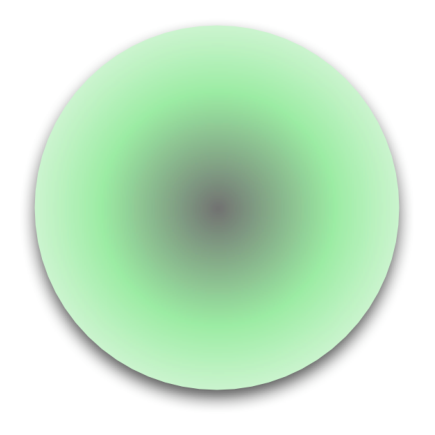
\includegraphics{orbitalS.eps}}
\vglue 0.2in
\hspace{1.5cm}\resizebox{9cm}{3cm}{ 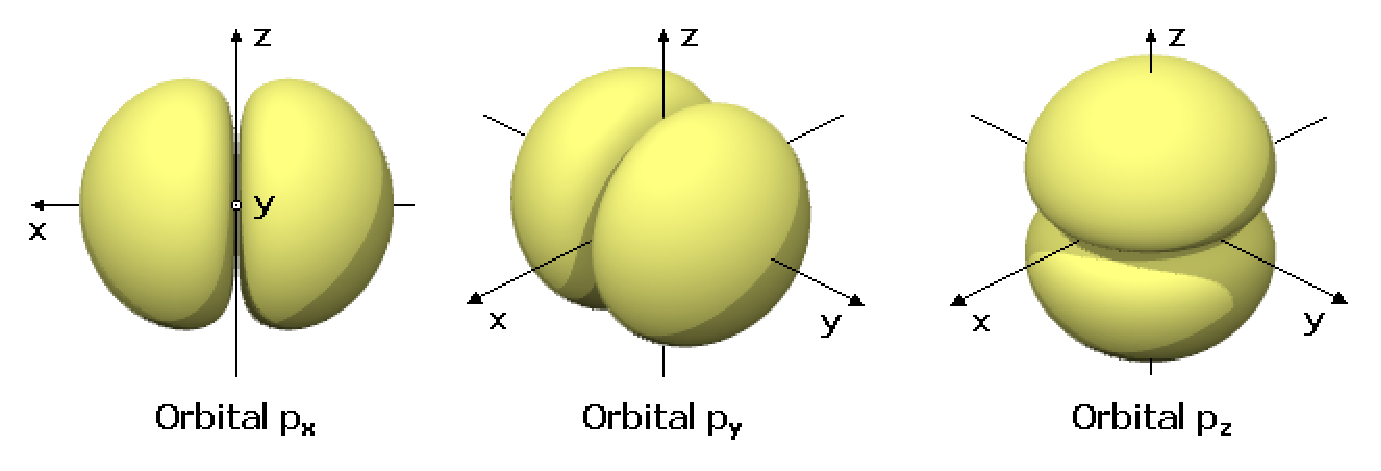
\includegraphics{orbitales_p.eps}}
%\vglue 0.05in
\caption[Orbitales $s$ y$p$]{Representaci\'on de un orbital tipo $s$ (parte superior)
y de un orbital $p$ (inferior)}
\label{fig3:1}
\end{figure}
\end{center}

\subsection{Configuraciones electr\'onicas}
Comenzando con el hidr\'ogeno y avanzando en el orden de n\'umero at\'o\-mi\-co
creciente, los \'atomos de helio, litio, berilio, etc., de cada uno de los elementos siguientes contiene un prot\'on y un electr\'on m\'as que los \'atomos
del elemento anterior.

Las estructuras electr\'onicas \index{estructuras@estructuras electr\'onicas} del  estado fundamental de los primeros 20 elementos quedan en un esquema regular. El
electr\'on \'unico del hidr\'ogeno est\'a en el primer nivel de energ\'{\i}a, como tambi\'en los dos electrones del helio. Las estructuras electr\'onicas para el
hidr\'ogeno y el helio son $1s^1$ y $1s^2$. El n\'umero m\'aximo de electrones en el primer de energ\'{\i}a es dos $(2n^2 = 2 \times 1^2 = 2)$. Por lo tanto, los dos
electrones llenan el primer nivel de energ\'{\i}a del helio.

Un \'atomo con tres electrones tendr\'a su tercer electr\'on en el segundo nivel de energ\'{\i}a, pues el primero s\'olo puede contener dos electrones. Por lo
anterior, el tercer electr\'on en el litio (n\'umero at\'omico 3) est\'a en el subnivel $2s$ del segundo nivel de energ\'{\i}a. El litio tiene la estructura
electr\'onica $1s^22s^1$. El \textbf{Cuadro~\ref{tabla3.3}} muestra la estructura electr\'onica de los primeros veinte elementos.

\begin{table}[ht]
\caption[Estructuras electr\'onicas]{Estructura electr\'onica de los primeros veinte
elementos}
\label{tabla3.3}
\begin{center}
{\small
 \begin{tabular}{lcl}\hline
\textbf{Elemento} & \textbf{N\'umero de} &\textbf{ Estructura} \\
    &       \textbf{electrones}& \textbf{electr\'onica}\\ \hline
H   &  1 & $1s^1$\\
He  &  2 & $1s^2$\\
Li  &  3 & $1s^22s^1$\\
Be  &  4 & $1s^22s^2$\\
B   &  5 & $1s^22s^22p^1$\\
C   &  6 & $1s^22s^22p^2$\\
N   &  7 & $1s^22s^22p^3$\\
O   &  8 & $1s^22s^22p^4$\\
F   &  9 & $1s^22s^22p^5$\\
Ne  & 10 & $1s^22s^22p^6$\\
Na  & 11 & $1s^22s^22p^63s^1$\\
Mg  & 12 & $1s^22s^22p^63s^2$\\
Al  & 13 & $1s^22s^22p^63s^23p^1$\\
Si  & 14 & $1s^22s^22p^63s^23p^2$\\
P   & 15 & $1s^22s^22p^63s^23p^3$\\
S   & 16 & $1s^22s^22p^63s^23p^4$\\
Cl  & 17 & $1s^22s^22p^63s^23p^5$\\
Ar  & 18 & $1s^22s^22p^63s^23p^6$\\
K   & 19 & $1s^22s^22p^63s^23p^64s^1$\\
Ca  & 20 & $1s^22s^22p^63s^23p^64s^2$\\ \hline 
\end{tabular}
}
\end{center}
\end{table}\index{estructuras@estructuras electr\'onicas!primeros veinte elementos} 

\subsection{S\'{\i}mbolos de Lewis}
El m\'etodo de puntos de Lewis para representar \'atomos propuesto por el qu\'{\i}\-mi\-co estadounidense G. N. Lewis \index{Lewis@\textbf{Lewis}!s\'{\i}mbolo}emplea el  s\'{\i}mbolo del elemento, y puntos gr\'a\-fi\-cos para representar electrones. El n\'umero de puntos que se colocan alrededor del s\'{\i}mbolo es igual al n\'umero de
electrones $s$ y $p$ del nivel externo de energ\'{\i}a del \'atomo. Los puntos pares representan electrones apareados, y viceversa, los puntos no en pares, electrones no apareados.
\newpage
\begin{example}
H$\cdot$ es el s\'{\i}mbolo de Lewis para un \'atomo de hidr\'ogeno, $1s^1$

 :\.B es el s\'{\i}mbolo de Lewis para un \'atomo de boro,
$1s^22s^22p^1$. En este caso el Boro  :\.B representa al n\'ucleo del
boro y a los electrones $1s^2$; los puntos representan s\'olo  a los
electrones $2s^22p^1$.
\end{example}

Cuando se tiene completa la capa de valencia con  ocho electrones se tiene un gas  \gloss[word]{gasesnobles}\index{gas!noble} que son un grupo de elementos qu\'{\i}micos con propiedades  similares. En condiciones normales de presi\'on y temperatura, son gases monoat\'omicos inodoros, incoloros y presentan muy poca reactividad qu\'{\i}mica.

\subsection{Energ\'{\i}a de ionizaci\'on y afinidad electr\'onica}

De acuerdo con el concepto de Bohr, existen electrones a varios niveles discretos de
energ\'{\i}a que dependen de la cantidad de energ\'{\i}a que ha absorbido el
\'atomo. Si se aplica suficiente energ\'{\i}a al \'atomo, es posible sacar
completamente (o expulsar) uno o m\'as electrones de su estructura, formando
as\'{\i} un ion positivo:
\begin{center}
\'atomo + energ\'{\i}a $\longrightarrow$ ion positivo + electr\'on (e$^-$)
\end{center}
La cantidad de energ\'{\i}a necesaria para quitar un electr\'on (e$^-$) a un \'atomo  a un ion se llama \textbf{energ\'{\i}a de \gloss[word]{ionizacion}}\index{energ\'{\i}a! de ionizaci\'on}. La energ\'{\i}a de \textit{primera} ionizaci\'on es la cantidad de energ\'{\i}a necesaria para sacar al primer electr\'on de un \'atomo; la energ\'{\i}a de \textit{segunda} ionizaci\'on es la necesaria para sacar al segundo electr\'on, y as\'{\i} sucesivamente.
\begin{table}
\caption[Energ\'{\i}as de ionizaci\'on]{Energ\'{\i}as de ionizaci\'on de algunos elementos}
\label{ionizacion}
\begin{center}
\begin{tabular}{l r r r r r}\hline
&\multicolumn{5}{c}{\textbf{Cantidades necesarias de energ\'{\i}a(kJ/mol)}}\\
\cline{2-6}
  Elemento &1o. e$^-$&2o. e$^-$&3o. e$^-$&4o.e$^-$&5o. e$^-$\\ \hline
H  &$1,314 $\\
He &$2,372 $& $5,247$\\
Li &$520   $& $7,297$ & $11,810$ \\
Be &$900   $& $1,757$ & $\mathbf{14,845}$ &$ 21,000$\\
B  &$800   $& $2,437$ & $ 3,657$ & $\mathbf{25,020}$&$ 32,810$\\
C  &$1,088$ & $2,352$ & $ 4,619$ &$  6,222$&  $\mathbf{37,800}$\\
Ne &$\mathbf{2,080}$ & $3,962 $& $ 6,376$ &  $9,376$& $ 12,190$\\
Na &$ 496$ & $\mathbf{4,565}$ & $ 6,912$ &  $9,540$&  $13,355$\\\hline
\multicolumn{6}{l}{\tiny Los valores se muestran en kilojoules por mol,
mostrando las energ\'{\i}as necesarias para sacar de}\\[-.1in]
\multicolumn{6}{l}{\tiny 1 a 5 electrones por \'atomo. 
Las negritas indica la energ\'{\i}a necesaria para sacar un electr\'on de
una}\\[-.1in]
\multicolumn{6}{l}{\tiny   estructura
electr\'onica de gas noble.}\\
\end{tabular}
\end{center}
\end{table}

Las energ\'{\i}a de ionizaci\'on se pueden expresar en t\'erminos de varias unidades de energ\'{\i}a, como electronvolts, kilojoules o kilocalor\'{\i}as por mol. En el siguiente ejemplo se expresa la energ\'{\i}a en kilojoule por mol (\kilo\joule/\mole), que indica el n\'umero de kilojoule necesarios para expulsar un electr\'on (e$^-$) de todos los \'atomos en un mol de \'atomos.
\begin{center}
\begin{tabular}{ccccccc}
Na &+& 494 \kilo\joule & $\longrightarrow$ &Na$^+$ &$+$ &e$^-$\\
{\scriptsize 1 mol de}&&&&{\scriptsize  1 mol de}&&{\scriptsize 1 mol de}\\[-.1in]
{\scriptsize \'atomos de sodio} &&&&{\scriptsize iones de sodio} & &{\scriptsize 
electrones}\\ 
\end{tabular}
\end{center}

El \textbf{Cuadro~\ref{ionizacion}} da las energ\'{\i}as de ionizaci\'on para la eliminaci\'on de uno a cinco electrones de varios elementos. As\'{\i} se necesitan 1314{\kilo\joule} para sacar un electr\'on de una mol de hidr\'ogeno, pero s\'olo se necesitan 494{\kilo\joule} para sacar el primer electr\'on de un mol de \'atomos de sodio. El \textbf{Cuadro~\ref{ionizacion}} muestra cantidades progresivamente mayores de energ\'{\i}a para expulsar al segundo, tercero, cuarto y quinto electrones. Esta secuencia es l\'ogica, por que la remoci\'on de electrones no disminuye al n\'umero de protones, o cantidad de carga, del n\'ucleo. Por lo tanto, los electrones restantes quedan sujetos m\'as fuertemente. El \textbf{Cuadro~\ref{ionizacion}} tambi\'en muestra que se necesita una energ\'{\i}a de ionizaci\'on extremadamente grande cuando se retira un electr\'on de una estructura de gas noble, lo cual demuestra la gran estabilidad de esa estructura.

En la tabla peri\'odica la energ\'{\i}a de primera ionizaci\'on disminuye generalmente con la colocaci\'on de arriba abajo, en cada una de las columnas conocidas como grupos  o familias.

De izquierda a derecha dentro de un per\'{\i}odo (o rengl\'on) de la tabla peri\'odica, la energ\'{\i}a de ionizaci\'on aumenta gradualmente, a pesar de algunas
irregularidades. Los gases nobles tienen valores relativamente altos, lo que confirma la no reactividad qui\'{\i}mica de esta familia y la estabilidad de una estructura de ocho electrones en el nivel externo de energ\'{\i}a.

Los \'atomos tienen \textbf{\gloss[word]{afinidadelectronica}}\index{afinidad!electronica@electr\'onica} -- esto es, capacidad para atraer electrones y formar iones negativos. \'Esta se puede definir como la cantidad de energ\'{\i}a absorbida o liberada cuando se agrega un electr\'on a un \'atomo para formar un ion negativo. Para la mayor parte de los elementos, se desprende calor cuando se agrega un electr\'on a un \'atomo.
\begin{center}
\'atomo + electr\'on $\longrightarrow$ ion negativo + energ\'{\i}a
\end{center}

La afinidad electr\'onica es una medida de la atracci\'on que ejerce un \'atomo  hacia un electr\'on -- en otras palabras, de la tendencia a formar un ion
negativo. El cloro, por ejemplo, es un elemento no met\'alico y tiene una fuerte tendencia a formar iones negativos. En consecuencia, la afinidad del cloro es alta.

\begin{tabular}{ccccccc}
Cl &+& e$^-$ & $\longrightarrow$& Cl$^-$ & + &384 {\kilo\joule}  (83 kcal)\\
{\scriptsize 1 mol de}&&{\scriptsize 1 mol de}&&{\scriptsize 1 mol de}\\[-.1in]
{\scriptsize \'atomos de cloro}&&{\scriptsize electrones}&&{\scriptsize iones
cloruro}\\
\end{tabular}

La afinidad electr\'onica tiende a ser alta en los no metales (en especial para los hal\'ogenos, ox\'{\i}geno y azufre) y baja en los metales. La tendencia general de la afinidad electr\'onica es aumentar de izquierda a derecha en cualquier periodo, y disminuir de arriba abajo en una familia de elementos.

\subsection[Electrones de valencia]{Electrones en la capa externa: electrones de
valencia}

Una propiedad importante de los elementos es su tendencia a formar una estructura con capa externa estable. Para muchos elementos, esta capa externa estable contiene ocho electrones (dos $s$ y seis $p$) que es id\'entica a la estructura electr\'onica externa de los gases nobles. Los \'atomos rearreglan su estructura electr\'onica para llegar a un estado de mayor estabilidad. Estos rearreglos se logran perdiendo, ganando o compartiendo electrones de otros \'atomos. Por ejemplo un \'atomo de hidr\'ogeno tiene la tendencia a aceptar otro electr\'on y as\'{\i} llegar a la estructura electr\'onica como la del gas noble helio; un \'atomo de fl\'uor puede adquirir un electr\'on m\'as para llegar a una estructura electr\'onica estable como la del ne\'on.

Los electrones en la capa externa de un \'atomo son responsables de la mayor parte de esta actividad electr\'onica, y se les llama \textbf{electrones de \gloss[word]{valencia}}\index{electrones de valencia}. En los s\'{\i}mbolos de Lewis con puntos, esos puntos representan los electrones de la capa externa, y por lo tanto tambi\'en representa a los electrones de valencia.

La regla del octeto\index{octeto!regla} es una regla pr\'actica que explica la formaci\'on del enlace qu\'{\i}mico de los elementos representativos en funci\'on de la configuraci\'on electr\'onica de su capa de valencia. Esta regla indica que, los \'atomos se combinan entre s\'{\i} de tal manera que cada \'atomo est\'e rodeado de ocho electrones en su capa de valencia (de all\'{\i} la denominaci\'on de ``octeto'').

\subsection[Electronegatividad y tipos de enlace]{Relaci\'on entre electronegatividad y tipos de enlace}


Cuando dos tipos diferentes de \'atomos comparten un par de electrones, un  \'atomo asume una carga parcial positiva y el otro una carga parcial negativa
entre s\'{\i}. Esta diferencia de cargas se representa porque los dos \'atomos  ejercen atracci\'on desigual hacia el par de electrones compartidos. La fuerza
de atracci\'on que un \'atomo de un elemento presenta hacia los electrones en  una mol\'ecula se llama \textbf{\gloss[word]{electronegatividad}}.
\index{electronegatividad} Los elementos difieren en sus electronegatividades. Por ejemplo, tanto el hidr\'ogeno como el cloro necesitan un electr\'on para formar
configuraciones electr\'onicas estables. Comparten un par de electrones en el cloruro de hidr\'ogeno. Como consecuencia, el par de electrones se desplaza hacia el
\'atomo de cloro, d\'andole una carga negativa parcial y dejando al \'atomo de hidr\'ogeno con una carga parcial positiva.

\subsubsection{Polaridad de enlace}
\'Atomos id\'enticos tienen electronegatividades id\'enticas. En la mol\'ecula
de hidr\'ogeno H$_2$  $$H:H$$ los \'atomos de hidr\'ogeno atraen por igual al par
electr\'onico. La distribuci\'on de carga electr\'onica es sim\'etrica con respecto
a los dos n\'ucleos; es decir, no est\'a m\'as cerca de un n\'ucleo que al otro. 
Como un enlace es e\-lec\-trost\'aticamente igual al otro, se dice que el enlace no
es \textit{polar}. \index{enlace!covalente!no polar} (Esto significa
exactamente que no tiene polos, o extremos diferentes). Por la misma raz\'on el
enlace  en la mol\'ecula del fl\'uor F:F es tambi\'en no polar. \textit{Los \'atomos
con electronegatividades id\'enticas forman enlaces covalentes no polares}.

Los \'atomos de diferentes elementos tienen diferentes electronegatividades. En la
mol\'ecula de fluoruro de hidr\'ogeno HF,  como el \'atomo de fl\'uor \textbf{F} tiene una
electronegatividad mayor que le del hidr\'ogeno \textbf{H}, el par electr\'onico est\'a
compartido desigualmente. La carga electr\'onica del par compartido est\'a m\'as
cerca del \'atomo de fl\'uor (el electr\'on se encuentra m\'as tiempo cercano al F que
al H). El enlace resultante tiene carga negativa acumulada en un extremo, y deja carga
positiva en el otro. (El n\'ucleo del hidr\'ogeno est\'a en el otro extremo y queda
en alguna forma expuesto por la p\'erdida de electrones). Un enlace covalente en el
cual el par electr\'onico es compartido desigualmente se dice que es un
\textit{enlace covalente polar} \index{enlace!covalente!polar}.

La \gloss[word]{polaridad} de un enlace, es decir, el grado al cual un par electr\'onico es desigualmente compartido, depende de la diferencia entre las
electrone\-gatividades de los dos \'atomos enlazados. Cuando la diferencia de las elec\-tro\-ne\-gatividades es grande, mayor es la polaridad en el enlace.

\subsubsection{Car\'acter i\'onico parcial}

 Cuando se enlazan dos \'atomos de gran diferencia de electronegatividad, el resultado se clasifica mejor como un enlace i\'onico. El enlace i\'onico puede considerarse como un enlace polar extremo, en el cual no se comparten esencialmente los electrones.\index{enlace!ionico@i\'onico}

En el \textbf{Cuadro~\ref{enlace}} se muestran las relaciones entre la diferencia de electronegatividad, el tipo de enlace, y grado de car\'acter i\'onico y covalente.
\index{enlace!covalente}
\begin{table}[thb]
\caption[Electronegatividades y enlaces]{Diferencia de electronegatividad, tipo y
car\'acter del enlace}
\label{enlace}
{\small \begin{tabular}{cccc}\hline
\textbf{Diferencia de}&&\textbf{Grado de car\'acter}&\textbf{Grado de car\'acter}\\
\textbf{electronegatividad}&\textbf{Tipo de enlace}&\textbf{Covalente}& 
\textbf{i\'onico}\\ \hline

Cero &Covalente no polar&$+$ & $-$ \\
   & $\downarrow$ &\\
 $\downarrow$ &Polar covalente&  $\downarrow$ & $\downarrow$ \\
  &  $\downarrow$ & \\
Grande & I\'onico & $-$ & $+$ \\ \hline
\end{tabular}}
\end{table}
\section {Alcanos, alquenos, alquinos y aro\-m\'a\-ti\-cos}

En esta secci\'on se estudian los principales grupos de hidrocarburos como son los 
alcanos, los alquenos, los alquinos y los aro\-m\'a\-ti\-cos. Se presenta el concepto de orbital
h\'{\i}brido co\-mo base para explicar la geometr\'{\i}a, la estructura y el
comportamiento qu\'{\i}mico de los compuestos de carbono. Se reconoce la estructura de
los alcanos, alquenos y alquinos con base en sus enlaces sencillos, dobles y triples, 
respectivamente. Se estudia con m\'as detenimiento la nomenclatura de los alcanos, ya
que \'esta sirve de base para los alquenos, alquinos y compuestos org\'anicos en
general.

Se muestrl fen\'omeno de isomer\'{\i}a que es caracter\'{\i}stico de los compuestos org\'anicos y se estudiar\'an las isomer\'{\i}as de cadena, de posici\'on y
geometr\'{\i}a (cis-trans).

La propiedades f\'{\i}sicas de alcanos, alquenos, alquinos y arom\'aticos se estudia en
forma global por tener propiedades semejantes.

\subsection{Hidrocarburos}
Los \textbf{\gloss[word]{hidrocarburos}} \index{hidrocarburos} son compuestos constituidos por \'atomos de carbono e hi\-dr\'o\-ge\-no unidos entre s\'{\i} mediante
enlaces covalentes. Se conocen varias clases de hidrocarburos. Esas clases son los alcanos, los alquenos, los al\-qui\-nos y los hidrocarburos arom\'aticos.

El benceno C$_6$H$_6$ es un hidrocarburo \textit{arom\'atico}.\index{benceno} Contiene
\'atomos de car\-bono en una estructura anular especial. Los compuestos que contienen el
 anillo del benceno se les conocen como\index{aromaticos@arom\'aticos}\textit{compuestos
arom\'aticos}. Se emplea el t\'ermino de \textit{\gloss[word]{alifatico}}\index{alif\'atico} para identificar compuestos con cadenas abiertas de \'atomos de
carbono. As\'{\i}, los alcanos, los alquenos y los alquinos de cadena abierta se les llama \textit{hidrocarburos alif\'aticos}. Los combustibles f\'osiles (gas natural,
petr\'oleo y carb\'on) son las principales fuentes de hidrocarburos. El gas natural es principalmente metano con pe\-que\-\~nas cantidades de etano, propano y butano. El petr\'oleo es una mezcla de hidrocarburos de la cual se separa la gasolina, el queroseno, el combust\'oleo, los aceites lubricantes, la parafina y el petrolato.

El alquitr\'an de hulla, que es un subproducto vol\'atil del proceso de fabricaci\'on de
coque a partir de carbones para la industria del acero, es fuente de muchas substancias
qu\'{\i}micas valiosas, incluyendo a compuestos arom\'aticos como el benceno, tolueno y
naftaleno.

\subsection{Hibridaci\'on del \'atomo de carbono}
\index{hibridacion@hibridaci\'on}
El carbono forma un sinn\'umero de compuestos en los que
sus \'atomos se enlazan covalentemente con otros cuatro \'atomos. el m\'as
simple de \'estos es el metano, CH$_4$. La configuraci\'on electr\'onica del
\'atomo de carbono en el estado fundamental es

\begin{center}
\begin{tabular}{rccccc}
C(Z=6):& $\underline{\uparrow \downarrow} $& $\underline{ \uparrow \downarrow}
$& $\underline{\uparrow \;} $ &$\underline{\uparrow \; }$
&$\underline{\quad}$\\[-.1in]
&&&\multicolumn{3}{c}{$\underbrace{\quad\quad\qquad\quad}$}\\
&$1s$&$2s$&\multicolumn{3}{c}{$2p$}\\
\end{tabular}
\end{center}
por esto el carbono aparece en capacidad de formar s\'olo dos enlaces covalentes
contribuyendo con cada uno de sus dos electrones no apareados para formar un par
compartido. Para la mol\'ecula de metileno (\ce{CH2}) de vida fugaz es mucho menos
estable que la de \ce{CH4}.

En la mol\'ecula de metano cada \'atomo de H est\'a localizado en la esquina de
un tetraedro regular. En el \ce{CH4} todas las longitudes de enlace son las mismas
y el \'angulo entre cada enlace \ce{C-H} y entre cada uno de los tres es el \textit{\'angulo
tetra\'edrico}, con un valor de $109.5^\circ$. 

El carbono evidentemente emplea todos sus cuatro electrones de valencia de modo
que puedan formarse cuatro enlaces C--H. No es demasiado dif\'{\i}cil ver c\'omo
el carb\'on forma cuatro enlaces. Suponga que uno de los dos electrones $2s$ es
promovido al orbital $2p$ vacante pero de mayor energ\'{\i}a.
\begin{center}
\begin{tabular}{rccccc}
C(Z=6):& $\underline{\uparrow \downarrow} $& $\underline{ \uparrow \;}
$& $\underline{\uparrow \;} $ &$\underline{\uparrow \; }$
&$\underline{\uparrow \;}$\\[-.1in]
&&&\multicolumn{3}{c}{$\underbrace{\quad\quad\qquad\quad}$}\\
&$1s$&$2s$&\multicolumn{3}{c}{$2p$}\\
\end{tabular}
\end{center}

Ahora el \'atomo de carbono est\'a en condiciones de formar cuatro enlaces $\sigma$ mediante la superposici\'on de sus orbitales $2s$ y $2p$ con los
orbitales $1s$ de los cuatro \'atomos de hidr\'ogeno. La dificultad aqu\'{\i} es que si el enlace ocurre de esa manera, la mol\'ecula de \ce{CH4} no ser\'{\i}a
tetra\'edrica. Si la estructura del metano determinada experimentalmente es tetra\'edrica ?`C\'omo podemos explicarla empleando los orbitales $s$ y $p$ del
carbono?. La respuesta es que el conjunto de orbitales $s$ y $p$ en el estado fundamental es reemplazado por un nuevo conjunto que es adecuado para formar
cuatro enlaces \textit{equivalentes}, cada uno en un \'angulo tetra\'edrico con respecto a los otros.

\gloss[nocite]{hibridacion}
Estos nuevos enlaces se les conoce como h\'{\i}bridos. Es la mezcla  o combinaci\'on de orbitales $s$ y $p$. El resultado es un orbital h\'{\i}brido, en el que la densidad de carga electr\'onica sufre un aumento. Este orbital h\'{\i}brido, llamado orbital\gloss[word]{orbitalsp}, es altamente direccional.

Podemos seguir la pista de la mezcla de los orbitales $2s$  y $2p$ en el carbono del siguiente modo:

\begin{tabbing}
\'Atomo en el estado fundamental \= $\qquad\underline{\uparrow \downarrow}\quad 
$\fbox{$\underline{\uparrow\downarrow}\quad
\underbrace{\underline{\uparrow\:\;}
\quad \underline{\uparrow\:\; }\quad \underline{\;\:\;}}$} \\
\>$\qquad 1s \quad\; 2s\quad \quad\quad 2p$\\
\>$\qquad \qquad \qquad \Downarrow$ {\footnotesize mezcla}\\
\'Atomo enlazado\>$\qquad\underline{\uparrow \downarrow}\quad 
$\fbox{$\underline{\uparrow \:\;}\quad
\underline{\uparrow \:\;}
\quad \underline{\uparrow\:\; }\quad \underline{\uparrow\:\;} $}\\
\>$\qquad 1s$  $\qquad \quad\quad 2sp^2$\\
\end{tabbing}
     
\subsection{Tipos de enlaces car\-bo\-no-car\-bono}\index{carbono!enlaces}
Con cuatro enlaces en la capa externa, el \'atomo de carbono siguiendo la regla del
octeto, forma cuatro enlaces sencillos covalentes compartiendo sus electrones con otros
\'atomos. Como ejemplo de \'esta tenemos las estruc\-turas del metano y del tetracloruro
de carbono un ejemplo de estos se muestra en la \textbf{Figura~\ref{fig3:2}}.

\begin{figure}[bht]
\hspace{1in} \resizebox{6cm}{6cm}{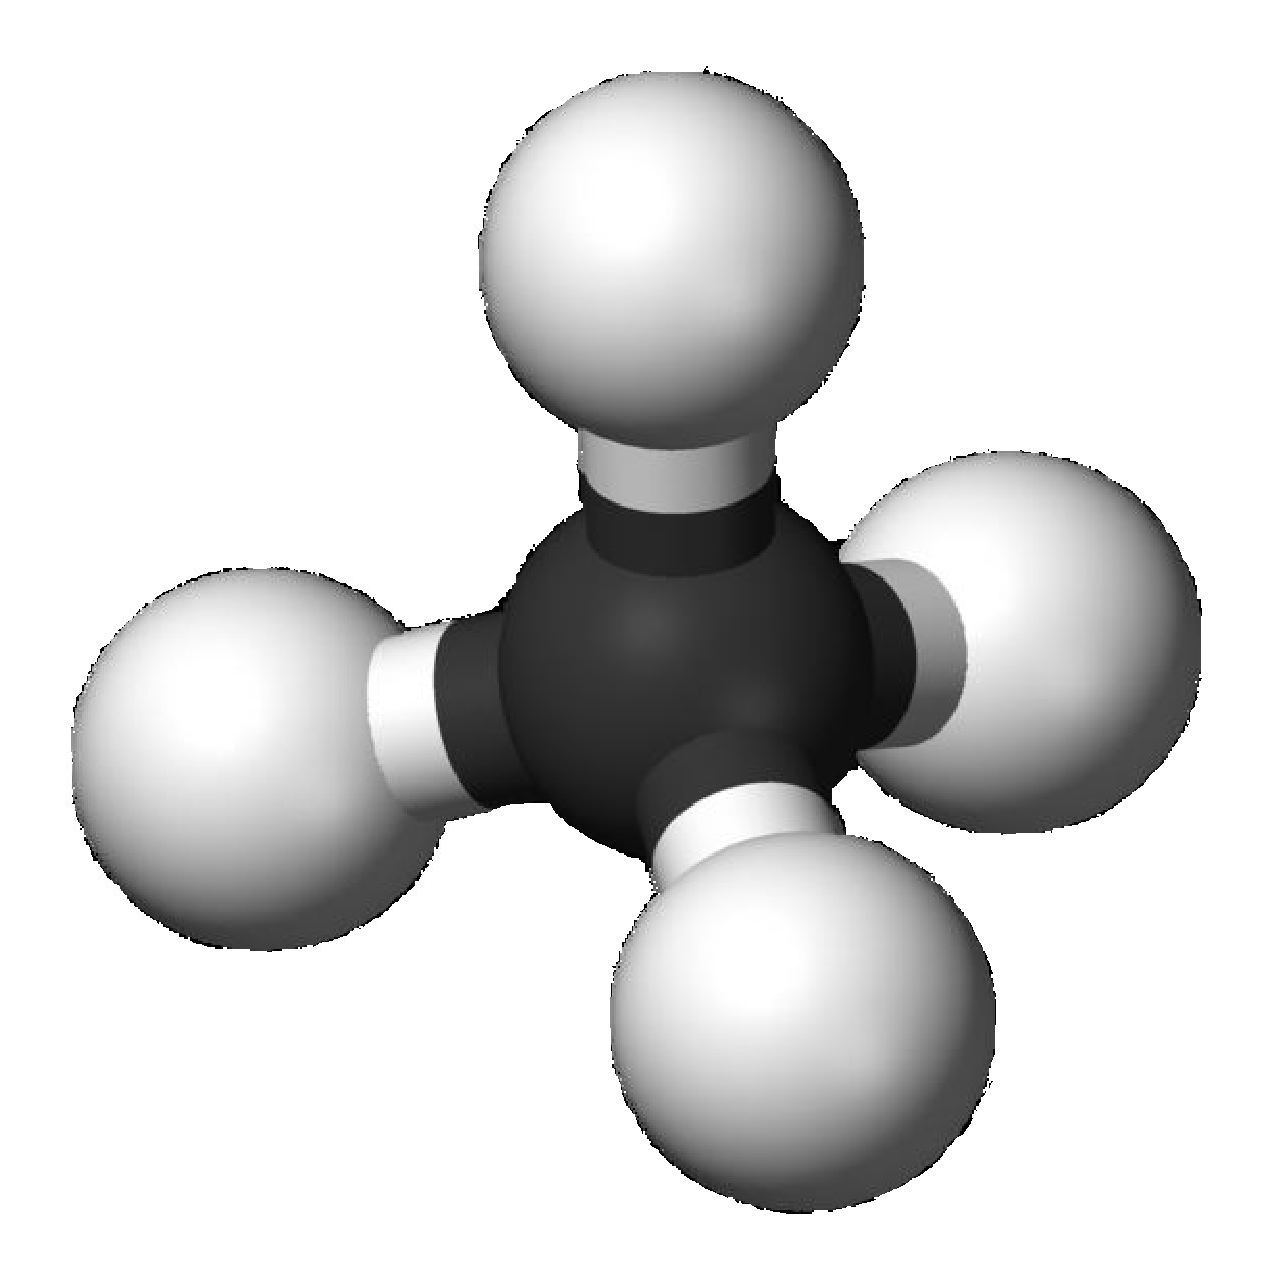
\includegraphics{metano3d.eps}}
\caption{Mol\'ecula de metano}
\label{fig3:2}
\end{figure}
En el metano, cada enlace se forma compartiendo electrones entre un \'atomo de carbono y un \'atomo de hidr\'ogeno.

La formaci\'on de los enlaces carbono-carbono se debe a la capacidad que tiene el \'atomo de carbono para compartir sus electrones con otros \'atomos iguales. Se pueden compartir uno, dos y tres pares de electrones entre dos \'atomos de carbono, formando respectivamente un enlace sencillo, un doble enlace y un triple enlace:
\begin{center}
\ce{C-C} \hskip .2in \ce{C\bond{2}C}  \hskip.2in  \ce{C\bond{3}C}  
\end{center}

Cada raya, en las f\'ormulas anteriores representa un enlace covalente. En el \textbf{Cuadro~\ref{enlaces}} se muestran algunos ejemplos de enlaces. El carbono, m\'as que ning\'un otro elemento, tiene la capacidad de formar cadenas de \'atomos enlazados covalentemente. Esta capacidad de enlazamiento es la principal raz\'on del gran n\'umero de compuestos org\'anicos.
\begin{center}
\begin{table}[htb]
\caption{Clases de compuestos org\'anicos}
\label{enlaces}
{\scriptsize \begin{tabular}{ l l l l l l }\hline
%\multicolumn{3}{l}{\textbf{clases de compuestos org\'anicos}}\\
& &Estructura& F\'ormulas &\multicolumn{2}{c}{\textbf{Nombre}}\\[-.01in]
 & F\'ormula &del grupo&estructurales\\[-.01in]
Clase   & general & funcional& de muestra& UIQPA$^a$ &Com\'un\\ \hline
Alcanos & RH &R$-$H & CH$_4$ &Metano & Metano\\
        &    &      & CH$_3$CH$_3$&Etano &Etano\\ \hline
Alquenos&R--CH$=$CH&$^\diagdown_\diagup $C$=$C$^\diagup_\diagdown$&CH$_2=$CH$_2$&
Etano & Etileno\\
       & &&CH$_3$CH$=$CH$_2$&Propeno&Propileno\\ \hline
Alquinos &R$-$\ce{CH\bond{3}C-H}& \ce{\bond{1}C\bond{3}C\bond{1}}&\ce{CH\bond{3}CH}&Etino &Acetileno\\
&&&CH$_3$C$\equiv$CH&Propino&Propileno\\
&&& &&Metilacetileno\\ \hline
Halogenuros&  &$-$X & CH$_3$Cl & Clorometano   &Cloruro de\\
de alquilo& &X$=$F,Cl, && &metilo\\
&&Br,I&CH$_3$CH$_2$Cl&Cloroetano &Cloruro de\\
&&&&& etilo\\[-.02in] \hline
\multicolumn{6}{l}{\scriptsize $^a$ IUPAC -- International Union of Pure and Applied Chemistry (Uni\'on Internacional de Qu\'{\i}mica Pura y Aplicada)}
\end{tabular}}
\end{table}
\end{center}

\subsection[Alcanos]{Hidrocarburos saturados: Alcanos}
Los \textbf{\gloss[word]{alcanos}}, \index{alcanos} son los hidrocarburos \textit{paraf\'{\i}nicos} o \textit{saturados}, estos compuestos tiene cadenas rectas o ramificadas de \'atomos de carbono, y entre dichos \'atomos s\'olo hay enlaces covalentes sencillos.
Estudiaremos con cierto detalle a los alcanos debido a que muchas otras clases de compuestos org\'a\-ni\-cos se les puede considerar como derivados de los alcanos. Por ejemplo, es necesario aprender los nombres de los primeros diez miembros de la serie de alcanos, por que tales denominaciones sirven de base para dar nombre a otras clases de compuestos.

\begin{table}[htd]
\begin{minipage}{\linewidth}
\caption[Alcanos caracter\'{\i}sticas]{Nombres, f\'ormulas y propiedades f\'{\i}sicas de los alcanos de cadena recta}
\label{alcanos}
\begin{center}
{\scriptsize \begin{tabular}{lllrr}\hline
 &\textbf{F\'ormula}& &\multicolumn{1}{c}{\textbf{Punto de}}
&\multicolumn{1}{c}{\textbf{Punto de}}\\
\textbf{Nombre}\footnote{Fuente: Wingrove \& Caret (1984)} & \textbf{molecular} &&\multicolumn{1}{c}{\textbf{ebullici\'on}}&
\multicolumn{1}{c}{\textbf{fusi\'on}}\\ &
C$_n$H$_{2n+2}$&\multicolumn{1}{c}{\textbf{F\'ormula estructural condensada}}
&\multicolumn{1}{c}{($^\circ$C)}&\multicolumn{1}{c}{($^\circ$C)}\\
\hline
Metano &\ce{CH4}    & \ce{CH4}       &$-161$&$-183$\\
Etano  &\ce{C2H6}   &\ce{CH3CH3}&$-88$&$-172$\\
Propano&\ce{C3H8}  &\ce{CH3CH2CH3}&$-45$&$-187$\\
Butano &\ce{C4H10} &\ce{CH3CH2CH2CH3}&$-1$&$-138$\\
Pentano&\ce{C5H12} &\ce{CH3CH2CH2CH2CH3}&$36$&$-130$\\
Hexano &\ce{C6H14} &\ce{CH3CH2CH2CH2CH2CH3}&$69$&$-95$\\
Heptano&\ce{C7H16} &\ce{CH3CH2CH2CH2CH2CH2CH3}&$98$&$-90$\\
Octano &\ce{C8H18} &\ce{CH3CH2CH2CH2CH2CH2CH2CH3}&$125$&$-57$\\
Nonano &\ce{C9H20} &\ce{CH3CH2CH2CH2CH2CH2CH2CH2CH3}&$151$&$-54$\\
Decano &\ce{C10H22}&\ce{CH3CH2CH2CH2CH2CH2CH2CH2CH2CH3}&$174$&$-30$\\ \hline \hline
\end{tabular}}
\end{center}
\end{minipage}
\end{table}

El \textit{metano} (\ce{CH4})\index{metano} es el primer miembro de esta serie de alcanos.
Los miembros que tiene dos, tres y cuatro \'atomos son \textit{etano}, \textit{propano} y \textit{butano}, respectivamente. Los nombres de los primeros cuatro alcanos son de origen com\'un y se deben memorizar; pero los nombres de los dem\'as, comenzando con el del quinto miembro (\textit{pentano}), se derivan de nombres griegos para los n\'umeros y son relativamente f\'aciles de recordar. En el \textbf{Cuadro~\ref{alcanos}} se presentan los nombres, f\'ormulas y algunas propiedades de los primeros diez  miembros de la serie.

Los compuestos sucesivos en la serie de los alcanos difieren entre s\'{\i} en su composici\'on, por un \'atomo de carbono y dos de hidr\'ogeno. Cuando cada miembro de una serie difiere del siguiente por un grupo \ce{CH2}, a la serie se la llama \textbf{serie hom\'ologa} \index{serie hom\'ologa}. Los miembros de una serie hom\'ologa son semejantes en su estructura, pero tienen una diferencia regular en su f\'ormula. Para todos los alcanos de cadena abierta, la f\'ormula general es \ce{C_nH_{2n+2}}, siendo $n$ el n\'umero de \'atomos en la mol\'ecula.


\begin{example}

As\'{\i} para el pentano, $n=5$, y $2n+2=12$, de manera que la f\'ormula es \ce{C5H12} y para el hexadecano, que es un alcano con $16$ \'atomos de carbono, la f\'ormula es \ce{C16H34}.
\end{example}
\subsubsection{Estructuras e isomer\'{\i}a}

La estructura molecular determina algunas de las propiedades de una substancia qu\'{\i}mica. La estructura es el modo en el que los \'atomos se encuentran unidos
entre s\'{\i} en una mol\'ecula. La mayor parte de las mol\'eculas org\'anicas se forman con pocos elementos: carbono, hidr\'ogeno, ox\'{\i}geno, nitr\'ogeno y los
hal\'ogenos. En estos compuestos el carbono posee cuatro valencias (tetravalente), el hidr\'ogeno una  (monovalente), el ox\'{\i}geno dos (bivalente) y los ha\-l\'o\-ge\-nos son monovalentes. Una forma de representar los enlaces es mediante las ra\-yas o barras fijas a cada \'atomo:

\begin{center}
\begin{picture}(85,14)
%
\put(1,7.5){\line(1,0){3}}
\put(5,6){C}
\put(8.5,7.5){\line(1,0){3}}
\put(6.5,9.5){\line(0,1){2.5}}
\put(6.5,2.5){\line(0,1){2.5}}
%
\put(15,6){H}
\put(18,7.5){\line(1,0){3}}
%
\put(25,7.5){\line(1,0){3}}
\put(28,6){O}
\put(31.5,7.5){\line(1,0){3}}
%
\put(38,7.5){\line(1,0){3}}
\put(41,6){N}
\put(44.5,7.5){\line(1,0){3}}
%
\put(50,6){Cl}
\put(54,7.5){\line(1,0){3}}
%
\put(59,6){Br}
\put(63,7.5){\line(1,0){3}}
%
\put(69,6){I}
\put(70.5,7.5){\line(1,0){3}}
%
\put(76,6){F}
\put(78.5,7.5){\line(1,0){3}}
%
\end{picture}

\end{center}
As\'{\i}, el carbono tendr\'a cuatro enlaces para otros \'atomos; el nitr\'ogeno tres;  el ox\'{\i}geno dos; y los hal\'ogenos e hidr\'ogeno, uno.

En un alcano cada \'atomo de carbono est\'a unido a otros cuatro \'atomos mediante cuatro enlaces covalentes sencillos. Las mol\'eculas de alcano contiene s\'olo enlaces carbono-carbono y carbono-hidr\'ogeno, y son esencialmente no polares.

Debido a esta baja polaridad, las mol\'eculas de alcano tienen muy poca atracci\'on intermolecular, y por lo tanto sus puntos de ebullici\'on son relativamente bajos en
comparaci\'on con otros compuestos org\'anicos de masa molecular semejante.

Para expresar la f\'ormula estructural correcta para el propano (\ce{C3H8}) se debe  determinar c\'omo colocar cada \'atomo  en la mol\'ecula. Un alcano s\'olo contiene
enlaces sencillos, y el carbono es tetravalente. Por lo tanto, cada \'atomo de carbono debe estar enlazado a cuatro \'atomos m\'as mediante enlaces \ce{C-C} o \ce{C-H}. El hidr\'ogeno es univalente y por lo tanto se debe enlazar s\'olo a un \'atomo de carbono mediante un enlace \ce{C-H}, ya que no existen los enlaces \ce{C\bond{-}H-C}, y un enlace \ce{H-H} s\'olo representa una mol\'ecula de  hidr\'ogeno. Con esta informaci\'on se encuentra que la \'unica estructura posible para el propano es:
%
\begin{center}
\begin{picture}(40,20 )
%Hidrogenos de los extremos
\multiput(2, 8)(29,0){2}{H}
%Enlaces al centro
\multiput(6, 9.5)(7,0){4}{\line(1,0){3}}
% Carbonos al centro
\multiput(10, 8)(7,0){3}{C}
% Enlaces e Hidrogenos parte superior
\multiput(11.5,12)(7,0){3}{\line(0,1){2}}
\multiput(10,15)(7,0){3}{H}
% Enlaces e hidrogenos parte inferior
\multiput(11.5, 5)(7,0){3}{\line(0,1){2}}
\multiput(10, 1)(7,0){3}{H}
%
\end{picture}
\end{center}


Sin embargo, es posible trazar dos f\'ormulas estructurales que co\-rres\-ponden a la f\'ormula molecular \ce{C4H10}  (butano):
\begin{center}
\begin{picture}(92,40)
%  Cadena central
\multiput( 1,15)(36,0){2}{H}
\multiput( 5,16.5)( 7,0){5}{\line(1,0){3}}
\multiput( 9,15)( 7,0){4}{C}
%
%  Enlaces parte superior e Hidrogenos
%
\multiput(10.5,19)(7,0){4}{\line(0,1){2}}
\multiput( 9,22)(7,0){4}{H}
%
%  Enlaces parte inferior e Hidrogenos
%
\multiput(10.5,12)(7,0){4}{\line(0,1){2}}
\multiput( 9, 8)(7,0){4}{H}
%
\put(12,3){n-Butano}

%  Cadena central
\multiput(49,15)(29,0){2}{H}
\multiput(53,16.5)( 7,0){4}{\line(1,0){3}}
\multiput(57,15)( 7,0){3}{C}
%
%  Enlaces parte superior e Hidrogenos
%
\put(58.5,19){\line(0,1){2}}
\put(65.5,19){\line(0,1){5}}
\put(72.5,19){\line(0,1){2}}
%
\put(57,22){H}
\put(64,25){C}
\put(71,22){H}
%
%  Enlaces parte inferior e Hidrogenos
%
\multiput(58.5,12)(7,0){3}{\line(0,1){2}}
\multiput(57,8)(7,0){3}{H}

\put(65.5,29){\line(0,1){4}}
\put(64,34){H}
\put(63.5,27){\line(-4,5){3.3}}
\put(67.5,27){\line( 4,5){3.3}}
\put(58,32){H}
\put(70,32){H}
\put(56,3){iso-Butano}
\end{picture}
\end{center}

Se muestran los compuestos  C$_4$H$_{10}$ con las f\'ormulas estructurales que se
indican, y que en realidad existen. El butano con la cadena no ramificada de carbono se
llama
\textit{butano normal} (que se abrevia $n-$butano); hierve a 0.5 $^\circ$C y funde a
$-138^\circ$C. El  butano de cadena ramificada se lama \textit{isobutano}; hierve a$-
11.7^\circ$C, y funde a $-159.5^\circ$C. Estas diferencias hacen notar que aunque
tienen a misma f\'ormula molecular, son substancias distintas.

El fen\'omeno en el que dos o m\'as compuestos tiene la misma f\'ormula molecular, pero
diferente arreglo en los \'atomos, se llama \textbf{isomerismo}. A los diferentes
compuestos con la misma f\'ormula se les conoce como \textbf{\gloss[word]{isomeros}}. 
\index{is\'omeros} El isomerismo es com\'un en los compuestos org\'anicos y es uno de
los motivos del gran n\'umero de compuestos conocidos. Hay tres is\'omeros del pentano,
5 is\'omeros del hexano, 9 is\'omeros del heptano, 18 is\'omeros del octano, 35 del
nonano y 75 del decano.

Para ahorrar tiempo y espacio en la escritura, se emplean con frecuencia las f\'ormulas
\textit{condensadas}.  En las f\'ormulas estructurales condensadas, los
\'atomos y grupos que est\'an fijos a un \'atomo de carbono se escriben a la derecha de
ese \'atomo.

  Por ejemplo la f\'ormula condensada del pentano es:  
\ce{CH3CH2CH2CH2CH3},
 o tambi\'en 
 \ce{CH3(CH2)_3CH3}

\subsubsection{Nomenclatura}\index{Nomenclatura!alcanos}\index{alcanos!nomenclatura}

Para asignarle un nombre a un compuesto al principio lo hac\'{\i}a quien lo hab\'{\i}a
sintetizado. Estos nombres no segu\'{\i}an alguna secuencia o sistematizaci\'on. Por
ejemplo el metano, se forma durante la descomposici\'on de la materia org\'anica en las
marisma o pantanos, as\'{\i} se le llam\'o como el \textit{gas de los pantanos}. Debido
a esto, a un solo compuesto se le asignaban diferentes nombres. De esta forma tenemos al
alcohol de las bebidas que se le conoce como \textit{alcohol}, \textit{alcohol
et\'{\i}lico, metil-carbinol, alcohol de granos, esp\'{\i}ritu de vinos} y
\textit{etanol.}\index{etanol}\index{alcohol}

A partir de una convenci\'on en Ginebra, el a\~no de 1892, se desarroll\'o un sistema internacional de nomenclatura de compuestos.

\begin{table}[hbt]
\caption[Grupos alquilo]{Nombres y f\'ormulas de algunos grupos alquilo}
\label{a-nom}
\begin{center}
\begin{tabular}{ll l l}\hline
\multicolumn{1}{c}{\textbf{F\'ormula}}&\multicolumn{1}{c}{\textbf{Nombre}}&
 \multicolumn{1}{c}{\textbf{F\'ormula}}&\multicolumn{1}{c}{\textbf{Nombre}}\\ \hline
CH$_3-$                & Metilo  &CH$_3($CH$_2)_4$CH$_2-$ & Hexilo \\
CH$_3$CH$_2-$          & Etilo   &CH$_3($CH$_2)_5$CH$_2-$ & Heptilo \\
CH$_3$CH$_2$CH$_2-$    & Propilo &CH$_3($CH$_2)_6$CH$_2-$ & Octilo \\
CH$_3($CH$_2)_2$CH$_2-$& Butilo  &CH$_3($CH$_2)_7$CH$_2-$ & Nonilo \\
CH$_3($CH$_2)_3$CH$_2-$& Pentilo &CH$_3($CH$_2)_8$CH$_2-$ & Decilo \\\hline
\end{tabular}
\end{center}
\end{table}
Para asignar sistem\'aticamente los nombres a los compuestos org\'anicos, es necesario  reconocer ciertos grupos \gloss[word]{alquilo} comunes. Los \textbf{grupos alquilo} \index{grupo!alquilo} tienen la f\'ormula general C$_n$H$_{2n+1}$ (teniendo un \'atomo menos de hi\-dr\'o\-ge\-no que el alcano correspondiente). Para obtener el nombre del grupo que se forma se usa el nombre del alcano correspondiente, se elimina su
terminaci\'on \textit{ano} y se sustituye por la terminaci\'on \textit{ilo}. En el \textbf{Cuadro~\ref{a-nom}} se dan  los nombres y f\'ormulas de algunos grupos alquilo. Com\'unmente se emplea la letra ``\textbf{R}'' en las f\'ormulas para indicar a cualquiera de los grupos alquilo posibles.

\hskip1.5in R = \ce{C_nH_{2n+1}} \hspace{.2in} (grupo alquilo)

Las siguientes reglas\index{Nomenclatura!reglas UIQPA} son las que se necesitan para dar
nombre a una gran cantidad de alcanos de acuerdo a el sistema
\gloss[short]{UIQPA} \footnote{Uni\'on Internacional de Qu\'{\i}mica Pura y Aplicada (International Union of Pure and Applied Chemistry)}. Y
son como sigue:
\begin{enumerate}
\item Seleccionar la cadena continua m\'as larga de \'atomos de carbono como compuesto
padre, y considerar a los otros grupos alquilo fijos a ella como cadenas de
ramificaci\'on o sustituyentes que han reemplazado a \'atomos de hidr\'ogeno del
hidrocarburo progenitor. Si se encuentran dos cadenas de igual longitud, se emplea la
que tiene mayor n\'umero de sustituyentes fijos a ella. El nombre del alcano
corresponde del nombre del compuesto originalmente precedido por los nombres de los
grupos alquilo fijos a \'el.
\item Numerar los \'atomos de carbono de la cadena del compuesto padre, comenzando por el
extremo m\'as pr\'oximo al primer \'atomo de carbono que contenga fijos a \'el un grupo
alquilo u otro grupo funcional, sustituyendo a  un \'atomo de hidr\'ogeno. Si el primer
sustituyente a partir de cada extremo queda en el carbono con el mismo n\'umero, se
procede hacia el siguiente sustituyente para determinar qu\'e extremo de la cadena se
emplea para comenzar la numeraci\'on.
\item Se da el nombre a cada grupo alquilo y se especifica su posici\'on en la cadena
de carbonos del compuesto padre mediante un n\'umero (por ejemplo: 3-metil significa un
grupo metilo fijo al \textbf{C} n\'umero 3).
\item Cuando se presenta la cadena fija ramificada con el mismo grupo  alquilo m\'as de
una vez, se indica esa repetici\'on con un prefijo (\textit{di}, \textit{tri},
\textit{tetra}, y as\'{\i} sucesivamente) escrito frente  al nombre del grupo alquilo
(por ejemplo, dimetil indica que existen dos grupos metilo).  Los n\'umeros indican las
posiciones de esos grupos alquilo se separan por na coma y se siguen de un gui\'on,
anteponi\'endolos al nombre (p.e. 2,3-dimetil).
\item Cuando existen varios grupos alquilo diferentes fijos al compuesto progenitor, se
enuncian en orden alfab\'etico. Por ejemplo, el etil antes que el metil en el
3-etil-4-metiloctano. Los prefijos no se consideran en el ordenamiento alfab\'etico
(etil viene antes de dimetil).
\end{enumerate}

Al compuesto siguiente se le llama generalmente isopentano. Su denominaci\'on de acuerdo con el sistema UIQPA ser\'a como sigue:

\begin{picture}(110,16)
\put( 1,9){CH$_3$}
\put( 9,10.5){\line(1,0){3}}
\put(13,9){CH$_2$}
\put(21,10.5){\line(1,0){3}}
\put(25,9){CH}
\put(32.5,10.5){\line(1,0){3}}
\put(37,9){CH$_3$}
\put(25,2){CH$_3$}
\put(26.5,6){\line(0,1){2}}

\put(50,9){o bien}
\put(45,2){\scriptsize 2-Metil butano}
\put(66,9){CH$_3$}
\put(74,10.5){\line(1,0){3}}
\put(78,9){CH}
\put(86,10.5){\line(1,0){3}}
\put(90,9){CH$_2$}
\put(98 ,10.5){\line(1,0){3}}
\put(102,9){CH$_3$}
\put(78,2){CH$_3$}
\put(79.5,6){\line(0,1){2}}

\setcounter{cm}{5}
\multiput( 2,13)(12,0){4}{\addtocounter{cm}{-1}
  \makebox(0,0)[b]{{\scriptsize \arabic{cm}}}}
\setcounter{cm}{0}
\multiput(67,13)(12,0){4}{\addtocounter{cm}{ 1}
  \makebox(0,0)[b]{{\scriptsize \arabic{cm}}}}
\end{picture}

La cadena continua m\'as larga contiene cuatro \'atomos de carbono. Por lo tanto, el compuesto padre es el butano y el compuesto se denomina como un derivado del butano. El grupo metilo (\ce{CH3}--)\index{metilo} fijo al carbono n\'umero 2 se usa como prefijo del butano, y el
``2'' indica el punto de fijaci\'on del grupo en la cadena but\'anica.

\subsection[Alquenos y Alquinos]{Hidrocarburos insaturados: Alquenos y alquinos}

Gran parte de los compuestos org\'anicos se sintetizan a partir de materiales
iniciales como: etileno, propileno, benceno, butileno, tolueno, xileno y metano. De esas
siete substancias mencionadas, todas, con excepci\'on del etano, son hidrocarburos no
saturados. tan s\'olo el etileno es la base de casi la mitad de los productos
petroqu\'{\i}micos.

Tanto los \textbf{\gloss[word]{alqueno}}\index{alquenos} y los
\textbf{\gloss[word]{alquino}} \index{alquinos} son hidrocarburos no saturados. Se
les dice no saturados, porque a diferencia de los alcanos, sus mol\'eculas no
contienen el n\'umero m\'aximo posible de \'atomos de hidr\'ogeno. Los alquenos tiene
dos \'atomos menos de hidr\'ogeno, y los alquinos tiene cuatro menos que los
correspondientes alcanos. Los alquenos (tambi\'en conocidos como hidrocarburos
\textit{olef\'{\i}nicos}) contiene al menos un doble enlace entre \'atomos de C
adyacentes. Los alquinos (\textit{acetil\'enicos}) contiene al menos un triple enlace
entre \'atomos adyacentes de carbono.

\subsubsection{Estructura}

El etileno (o eteno) es el alqueno m\'as simple, CH$_2=$CH$_2$, y el alquino m\'as
sencillo es el acetileno (o etino), \ce{CH\bond{3}CH}, (\textbf{F\/igura~\ref{fig3:3}}). El etileno y el
acetileno son los primeros miembros en las series hom\'ologas en las que las f\'ormulas
de los miembros sucesivos difieren por incrementos de CH$_2$. Por ejemplo,
\ce{CH2\bond{2}CH2}, \ce{CH3CH\bond{2}CH2} y \ce{CH3CH2CH\bond{2}CH2}.

\begin{figure}[htb]
\hspace{.5cm}\resizebox{6cm}{4cm}{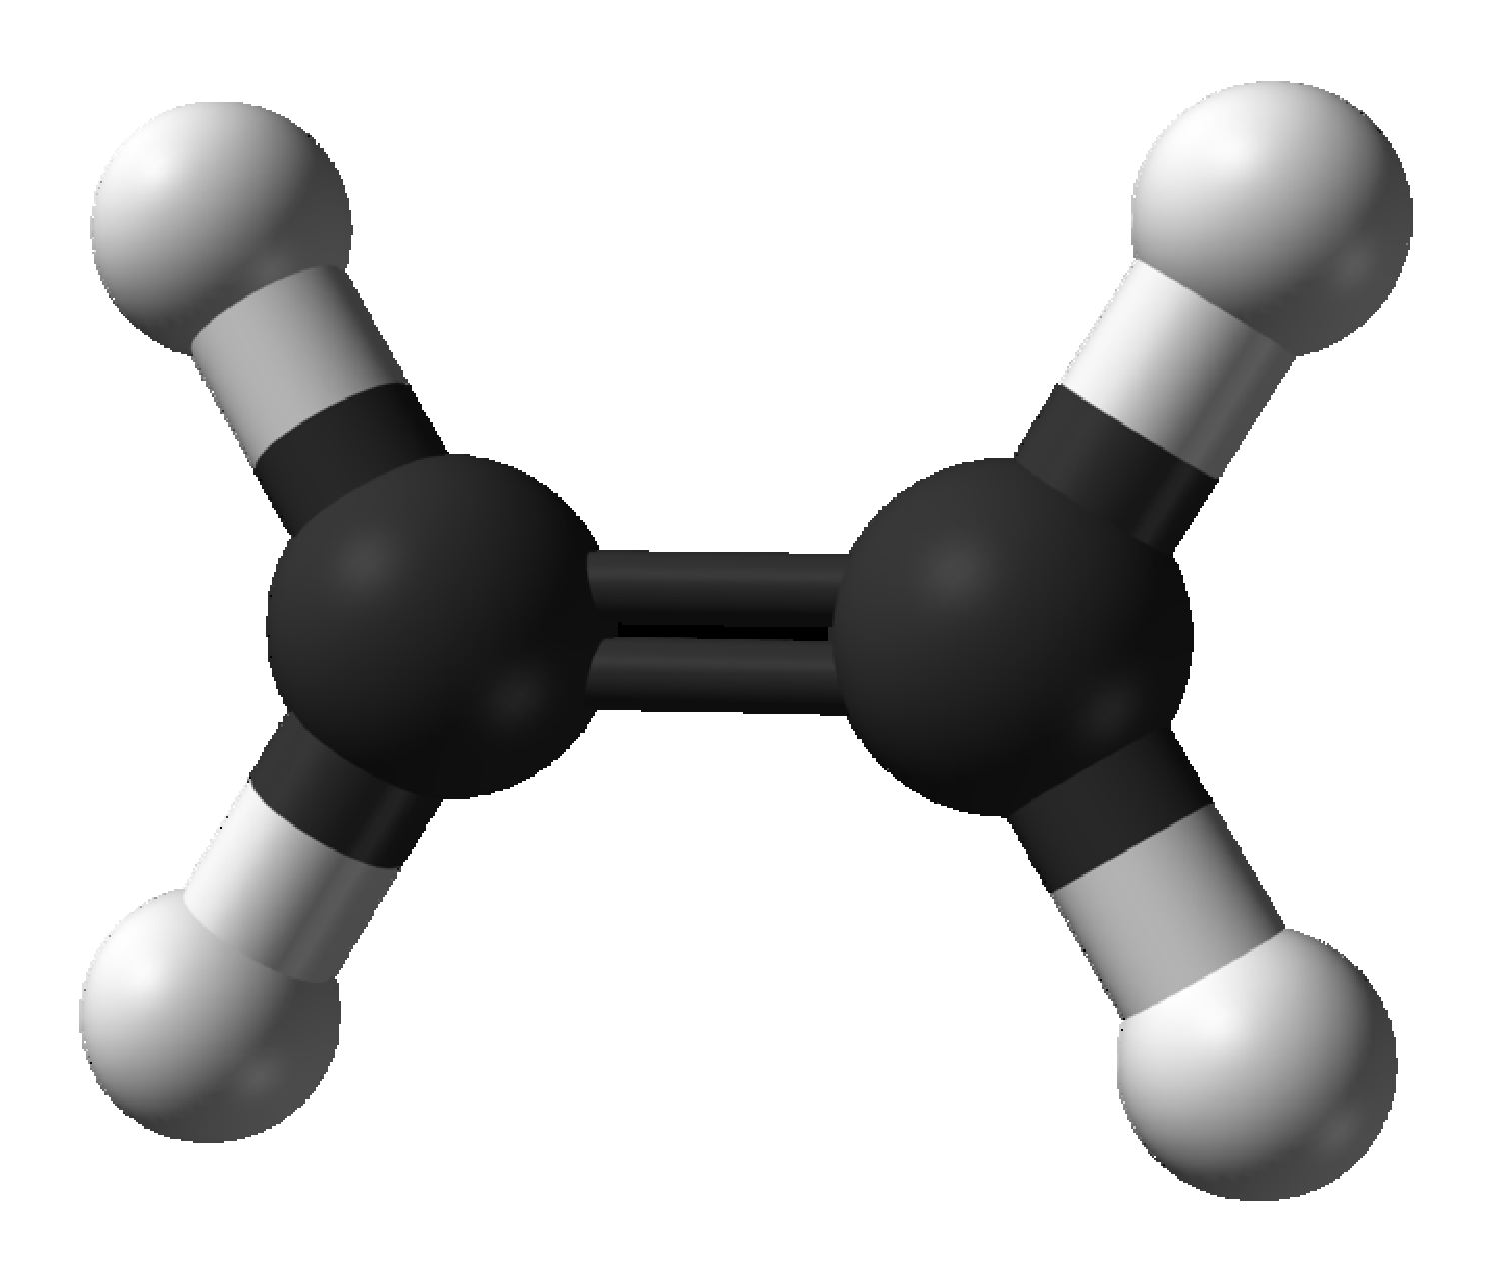
\includegraphics{etileno.eps}}
\resizebox{6cm}{2cm}{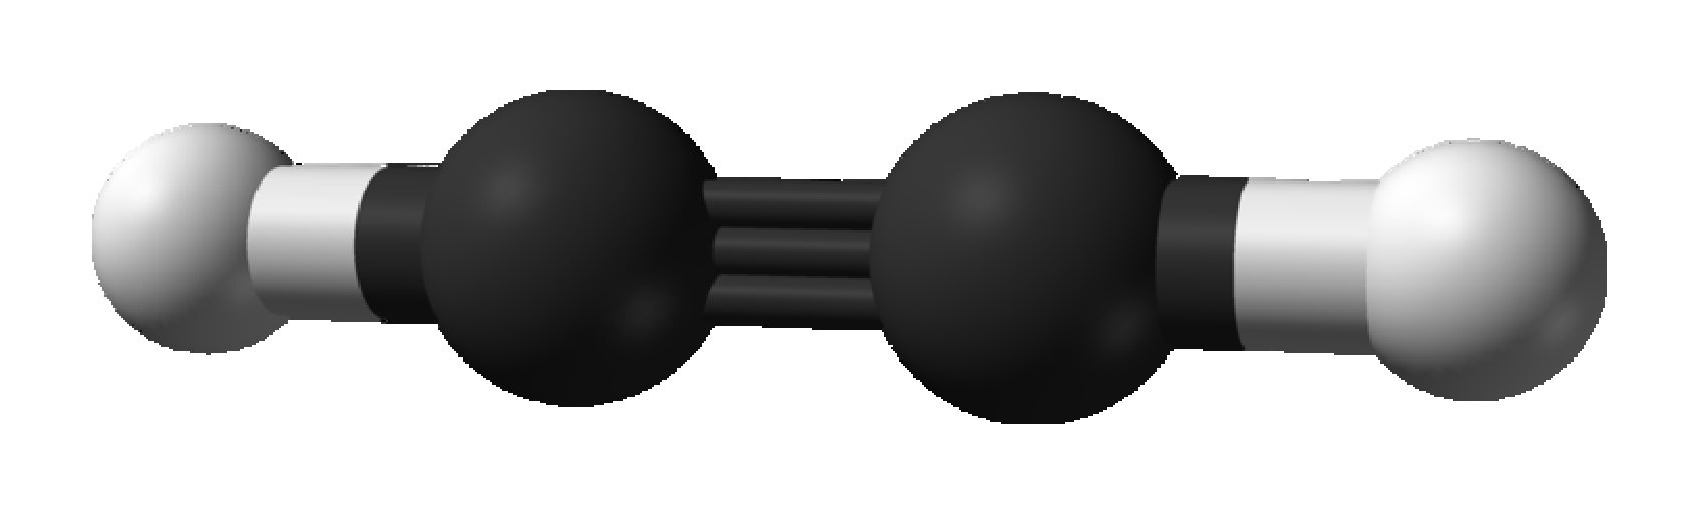
\includegraphics{acetileno.eps}}
\caption[Mol\'eculas de etileno y acetileno]{Mol\'eculas de etileno (izq.) y acetileno (der.)}
\label{fig3:3}
\end{figure}

\subsubsection{Propiedades f\'{\i}sicas}

Las mol\'eculas de los alquenos, como las de los alcanos, tienen muy poca polaridad. Por lo tanto, las propiedades f\'{\i}sicas de los alquenos son muy semejantes a las de los correspondientes hidrocarburos saturados. Los alquenos que contienen dos a cuatro \'atomos de carbono son gases; los que tiene 5 a 18 \'atomos de carbono son l\'{\i}quidos; y los que tiene m\'as de 18 carbonos son s\'olidos. Son relativamente poco solubles en agua, pero se disuelven en \'acido sulf\'urico concentrado. En el \textbf{Cuadro~\ref{prop:1}} se resumen algunas de la propiedades de los alquenos m\'as comunes.

\begin{table}[hbt]
\begin{minipage}{\linewidth}
\caption[Propiedades de Insaturados]{Propiedades f\'{\i}sicas de varios alquenos y alquinos}
\label{prop:1}
\begin{center}
{\small \begin{tabular}{lr r}\hline
&\multicolumn{1}{c}{\textbf{Punto de}}&
\multicolumn{1}{c}{\textbf{Punto de }}\\ 
&\multicolumn{1}{c}{\textbf{ fusi\'on}}&
\multicolumn{1}{c}{\textbf{ ebullici\'on}}\\
\multicolumn{1}{c}{\textbf{Compuesto\footnote{Fuente: Wingrove \& Caret (1984)}}} &\multicolumn{1}{c}{$^\circ$\textbf{C}}&
\multicolumn{1}{c}{$^\circ$\textbf{C}}\\\hline
 Etileno &                  $-169$& $-104$\\
 Propileno&               $-185$& $-48$ \\
1-Buteno&                 $-185$& $-6$\\
2-Buteno (\textit{cis})&  $-139$& $+4$ \\
2-Buteno (\textit{trans})&$-106$& $+1$ \\
1-Penteno                &$-165$& $+30$ \\
1-Hexeno                & $-140$& $+64$\\
ciclo penteno           &$-135$& $+44$\\
 Acetileno                 &$  -82$& $-57$\\
 Propino                   &$-103$& $-23$\\
 1-Butino                  &$-126$& $+8$\\
2-Butino                 &$   -32$& $+27$\\ 
1-Pentino                &$-106$& $+40$\\
2-Pentino                &$-109$& $+56$\\
1-Hexino                 &$-132$& $+71$\\
2-Hexino                 &$  -90$& $+84$\\
\hline \hline
\end{tabular}}
\end{center}
\end{minipage}
\end{table}


\subsubsection{Nomenclatura}
\index{alquenos!nomenclatura}
\index{alquinos!nomenclatura}
\index{Nomenclatura!alquenos}
\index{Nomenclatura!alquinos}

Se fabrican grandes cantidades de alquenos por desintegraci\'on (o \gloss[word]{craqueo}) y \index{craqueo} deshidrogenaci\'on\index{deshidrogenacion@deshidrogenación}  de alcanos en el procesamiento de petr\'oleos crudos. 

En el \textbf{Cuadro~\ref{insat:1}} da los nombres de las f\'ormulas para varios alquenos y alquinos comunes.
\begin{table}[htb]
\caption[Grupos Insaturados]{Nombres y f\'ormulas de varios alquenos y alquinos}
\label{insat:1}
\begin{center}
{\small \begin{tabular}{lll}\hline
\multicolumn{1}{c}{\textbf{F\'ormula}}&\multicolumn{1}{c}{\textbf{Nombre UIQPA}}&
\multicolumn{1}{c}{\textbf{Nombre com\'un}}\\ \hline
\ce{CH2\bond{=}CH2}                 & Eteno & Etileno\\
\ce{CH3-CH\bond{=}CH2}          &Propeno  & Propileno\\
\ce{CH3-CH2-CH\bond{=}CH2}   & 1-Buteno & Butileno\\
\ce{CH3-CH\bond{=}CH-CH3}     & 2-Buteno \\
\\
\ce{CH\bond{3}CH}                  & Etino & Acetileno \\
\ce{CH3-C\bond{3}CH}   & Propino  &  Metilacetileno\\
\ce{CH3-CH2-C\bond{3}CH} & 1-Butino & Etilacetileno\\
\ce{CH3-C\bond{3}C-CH3}& 2-Butino & Dimetilacetileno\\ \hline \hline

\end{tabular}}
\end{center}
\end{table}

Los nombres de los alquenos y alquinos se derivan de los nombres de los correspondientes alcanos. Para dar nombre a un alqueno (o alquino) de acuerdo con el sistema UIQPA:

\begin{enumerate}
\item Se selecciona la cadena carbono-carbono m\'as larga que contenga al doble o triple enlace.
\item Se nombra al compuesto padre obteniendo como si se tratara de un alcano, pero se cambia la terminaci\'on \textit{ano} por la terminaci\'on \textit{eno}, si se trata de un alqueno, o \textit{ino} para un alquino. Por ejemplo el propano cambia a propeno o a propino:

{\scriptsize \begin{tabular}{ccc}
\ce{CH3-CH2-CH3}& \ce{CH3-CH\bond{=}CH2}    &\ce{CH3-C\bond{3}CH}  \\
\textit{Propano} & \textit{Propeno} &\textit{Propino}\\
\end{tabular}}

\item Se numera la cadena de carbonos del compuesto progenitor comenzando con el extremo m\'as cercano al doble o triple enlace. Se usa el menor de los dos n\'umeros que se obtengan en los \'atomos con el doble o el triple enlace. Se coloca este n\'umero frente al nombre del alqueno o alquino; por ejemplo, 2-buteno que quiere decir que el doble enlace carbono-carbono se encuentra entre C-2 y C-3.

\item Las cadenas laterales y dem\'as grupos se tratan como cuando se dan nombres a los alcanos. Se nombra el grupo sustituyente, y se especifica su posici\'on en la cadena principal como n\'umero.

\end{enumerate}

\subsubsection{F\'ormulas generales} Para describir tanto los alquenos como los alquinos se pueden utilizar ecuaciones condensadas generales como las siguientes:

La f\'ormula general de alquenos es: \textbf{C}$_n$\textbf{H}$_{2n}$

La f\'ormula general de alquinos es:  \textbf{C}$_n$\textbf{H}$_{2n-2}$

\begin{exercises}
\exer  Nombra los siguientes compuestos:
\begin{figure}[ht]
\sidebyside{
\begin{picture}(50,16)
\put( 1,12){(a) CH$_3$CHCH}

\put(14,9){\line(0,1){2}}
\put(13.5,5){CH$_3$}

\put(24.5,12.5){\line(1,0){3}}
\put(24.5,13.5){\line(1,0){3}}
\put(29,12){CHCHCH$_3$}
\put(35,9){\line(0,1){2}}
\put(34.5,5){CH$_2$CH$_3$}
\put(12,0){{\scriptsize Resp:  (a) 2,5-dimetil-3-hepteno }}
\end{picture}
}
{
\begin{picture}(50,16)
\put(1,12){(b) CH$_3$C$\equiv$CCHCH$_2$CH$_2$CH$_2$CH$_3$}

\put(22.5, 9){\line(0,1){2}}
\put(22,5){CH$_2$CH$_3$}
\put(16,0){{\scriptsize Resp:  (b) 4-etil-2-octilo}}
\end{picture}
%\caption{Resp:  (b) 4-etil-2-octilo }
}
\end{figure}

\end{exercises}




\subsection{Hidrocarburos arom\'aticos}

El benceno\index{benceno} y todas las substancias que tienen estructuras y propiedades qu\'{\i}\-mi\-cas
semejantes a \'este, se clasifican como \textbf{hidrocarburos arom\'aticos}
\index{hidrocarburos!arom\'aticos}. La palabra \textit{arom\'atico} se refiere al olor muy agradable que presentan muchas de esas substancias. El benceno, es la substancia que identifica a los arom\'aticos, fue aislado por primera vez por Michel Faraday en 1825; posterior\-men\-te se estableci\'o su formula molecular, \ce{C6H6}.  La estructura  molecular que explicar\'{\i}a las propiedades del benceno fue un problema dif\'{\i}cil para los qu\'{\i}micos de mediados del siglo XIX.

En 1865, August Kekul\'e\index{Kekule@Kekulé} propuso que los \'atomos de carbono en la mol\'e\-cula del benceno est\'an agrupados en un anillo de seis miembros con un \'atomo de hidr\'ogeno \textbf{H} enlazado a cada uno y con tres doble enlaces carbono-carbono:

\begin{picture}(60,42)(-10,0) % Molecula de benceno (izq)
\put(1,10){H}                  %Hidrogeno izq inferior
\put(9,16){\line(-5,-4){4}}       % Enlace C-H inf izq
\put(9.5,15){C}                % Carbono izq inf
\put(10.5,19){\line(0,1){4}}      % Doble  C=C centro izq(i)
\put(11.5,19){\line(0,1){4}}      % Doble  C=C centro izq(d)
\put(9.5,24){C}                % Carbono izq sup
\put(9,26){\line(-5,4){4}}        % Enlace C-H sup izq
\put(1,28.5){H}                % Hidrogeno izq sup
\put(13.5,26 ){\line(5,4){4}}     % Enlace C-C sup izq
\put(18,28.5){C}               % Carbono centro superior
\put(25.5,26) {\line(-5,4){4}}    % Enlace C=C der sup{s}
\put(26,27){\line(-5,4){4}}       % Enlace C=C der sup{i} 

\put(26.5,24){C}               % Carbono der sup
\put(28,19){\line(0,1){4}}        % Enlace C-C centro der
\put(30,26 ){\line(5,4){4}}       % Enlace C-H der sup
\put(34.5,28.5){H}             % Hidrogeno der sup

\put(26.5,15){C}               % Carbono der inf
\put(30,16){\line(5,-4){4}}       % Enlace C-H inf der
\put(34.5,10){H}               % Hidrogeno der inf

\put(19.5,32.5){\line(0,1){3}}    % Enlace C-H centro sup
\put(18,36){H}                 % Hidrogeno centro sup

\put(13.5,16){\line(5,-4){4}}     % Enlace C-C izq
\put(18,10){C}                 % Carbono centro inferior
\put(26,16){\line(-5,-4){4}}   %  Enlace C=C inf der(s)
\put(26.5,15){\line(-5,-4){4}} %  Enlace C=C inf der(i)

\put(19.5,6){\line(0,1){3}}       % Enlace C-H centro inf
\put(18, 2){H}                 % Hidrogeno centro inf

\put(42,20){{\LARGE $\rightleftarrows$}}

%\put(50,0){\line(0,1){42}}
\end{picture}
\begin{picture}(50,45)  % Molecula de benceno (der)
\put(   1,  10){H}             % Hidrogeno izq inferior
\put(   1,28.5){H}             % Hidrogeno izq sup
\put(34.5,28.5){H}             % Hidrogeno der sup
\put(34.5,  10){H}             % Hidrogeno der inf
\put(18  ,   2){H}             % Hidrogeno centro inf
\put(18  ,  36){H}             % Hidrogeno centro sup

\put(9.5,15){C}                % Carbono izq inf
\put(9.5,24){C}                % Carbono izq sup
\put(18,28.5){C}               % Carbono centro superior
\put(18,10){C}                 % Carbono centro inferior
\put(26.5,24){C}               % Carbono der sup
\put(26.5,15){C}               % Carbono der inf

\put(9,16){\line(-5,-4){4}}       % Enlace C-H inf izq
\put(9,26){\line(-5,4){4}}        % Enlace C-H sup izq
\put(19.5,32.5){\line(0,1){3}}    % Enlace C-H centro sup
\put(19.5,6){\line(0,1){3}}       % Enlace C-H centro inf
\put(30,26 ){\line(5,4){4}}       % Enlace C-H der sup
\put(30,16){\line(5,-4){4}}       % Enlace C-H inf der

\put(13  ,27  ){\line( 5, 4){4}}  % Enlace C=C sup izq(s)
\put(13.5,26  ){\line( 5, 4){4}}  % Enlace C=C sup izq(i)
\put(11  ,19  ){\line( 0, 1){4}}  % Enlace C-C centro izq
\put(13.5,15.5){\line( 5,-4){4}}  % Enlace C=C izq inf(s) 
\put(13  ,14.5){\line( 5,-4){4}}  % Enlace C=C izq inf(i)
\put(26  ,26.5){\line(-5, 4){4}}  % Enlace C-C der sup
\put(27.5,19  ){\line( 0, 1){4}}  % Enlace C=C centro der(d)
\put(28.5,19  ){\line( 0, 1){4}}  % Enlace C=C centro der(i)
\put(26  ,15.5){\line(-5,-4){4}}  % Enlace C-C inf der

\end{picture}

El benceno no participa f\'acilmente en las reacciones de adici\'on como todo alqueno  t\'{\i}pico. Por ejemplo, el benceno no decolora r\'apidamente las soluciones de bromo. En vez de ello, el comportamiento qu\'{\i}mico del benceno se asemeja al de un alcano. Sus reacciones t\'{\i}picas son del tipo de sustituci\'on, en donde un \'atomo  de hidr\'ogeno es sustituido por otro grupo, por ejemplo,
\reaction*{C6H6 + Cl2 ->[Fe] C6H5Cl + HCl}

Las teor\'{\i}as modernas indican que la mol\'ecula del benceno es un h\'{\i}brido de las dos estructuras de Kekul\'e anteriores.

Por comodidad, las mol\'eculas de benceno se representan con una de las siguientes
formas:

\hskip1.25in\begin{picture}(20,16)
\put(11  ,10  ){\line( 2, 1){4}}      % Enlace C=C sup izq(s)
\put(11.5, 9.5){\line( 2, 1){3.6}}    % Enlace C=C sup izq(i)
\put(11  , 5.5  ){\line( 0, 1){4.5}}  % Enlace C-C centro izq
\put(11.6, 6){\line( 2,-1){3.6 }}     % Enlace C=C izq inf(s) 
\put(11 , 5.5){\line( 2,-1){4}}       % Enlace C=C izq inf(i)
\put(19  ,10 ){\line(-2, 1){4}}       % Enlace C-C der sup
\put(19  , 5.5){\line( 0, 1){4.5}}    % Enlace C=C centroder(d)
\put(18.5, 6  ){\line( 0, 1){3.5}}    % Enlace C=C centro der(i)
\put(19  , 5.5){\line(-2,-1){4}}      % Enlace C-C inf der
\put(10,0){A}
%\put(20,0){\line(0,1){16}}
\end{picture}
\begin{picture}(20,16)
\put(11  ,10  ){\line( 2, 1){4}}      % Enlace C-C sup izq(s)
\put(11  , 5.5  ){\line( 0, 1){4.5}}  % Enlace C-C centro izq
\put(11 , 5.5){\line( 2,-1){4}}       % Enlace C-C izq inf(i)
\put(19  ,10 ){\line(-2, 1){4}}       % Enlace C-C der sup
\put(19  , 5.5){\line( 0, 1){4.5}}    % Enlace C-C centroder(d)
\put(19  , 5.5){\line(-2,-1){4}}      % Enlace C-C inf der
\put(15.1, 7.8){\circle{6.3}}
\put(10,0){B}
\end{picture}

En ambas representaciones, se sobreentiende que hay un \'atomo de carbono y de  hidr\'ogeno en cada esquina del hex\'agono. Las estructuras anteriores se emplean para representar las f\'ormulas estructurales de los derivados del benceno; esto es, las substancias en las que se han sustituido uno o m\'as \'atomos de hidr\'ogeno en el anillo por otros \'atomos o grupos. Por ejemplo, el clorobenceno\index{clorobenceno} (C$_6$H$_5$Cl) se escribe de las siguiente manera:

\hskip0.8in\begin{picture}(35,16)(-10,0)
\put(21  ,10  ){\line( 2, 1){4}}      % Enlace C-C sup izq(s)
\put(21  , 5.5  ){\line( 0, 1){4.5}}  % Enlace C-C centro izq
\put(21 , 5.5){\line( 2,-1){4}}       % Enlace C-C izq inf(i)
\put(29  ,10 ){\line(-2, 1){4}}       % Enlace C-C der sup
\put(29  , 10){\line( 2, 1){3.6}}       % Enlace del Cloro
\put(33.2, 11){{\scriptsize Cl}}
\put(29  , 5.5){\line( 0, 1){4.5}}    % Enlace C-C centroder(d)
\put(29  , 5.5){\line(-2,-1){4}}      % Enlace C-C inf der
\put(25.1, 7.8){\circle{6.3}}
\put(15,0){{\footnotesize Clorobenceno, C$_6$H$_5$Cl}}
\end{picture}

\subsubsection{Nomenclatura}
\index{arom\'aticos!nomenclatura}
\index{Nomenclatura!arom\'aticos}

Un benceno sustituido se obtiene reemplazando uno o m\'as de sus \'atomos de H por otro \'atomo o grupo de \'atomos. As\'{\i}, un benceno monosustituido\index{benceno!monosustituido} tiene la f\'ormula \ce{C6H5-G} siendo G el grupo que reemplaza a un \'atomo de hidr\'ogeno. Debido a que todos los \'atomos de hidr\'ogeno en el benceno son equivalentes, no importa en qu\'e esquina del anillo est\'e e grupo monosustituyente.

\paragraph{Bencenos monosustituidos} A algunos de los bencenos monosustituidos se les da el nombre a\~nadiendo el del grupo sustituyente como prefijo a la palabra \textit{benceno}. Se escribe as\'{\i} el nombre en una sola palabra. A continuaci\'on \index{nitrobenceno}\index{etilbenceno} \index{bromobenceno}
presentamos algunos ejemplos:

\begin{picture}(25,20)
\put( 5  ,10  ){\line( 2, 1){4}}      % Enlace C-C sup izq(s)
\put( 5  , 5.5  ){\line( 0, 1){4.5}}  % Enlace C-C centro izq
\put( 5 , 5.5){\line( 2,-1){4}}       % Enlace C-C izq inf(i)
\put(13  ,10 ){\line(-2, 1){4}}       % Enlace C-C der sup
\put( 9.1, 12){\line( 0, 1){2}}       % Enlace del Nitrilo
\put( 8, 15){{\footnotesize NO$_3$}}
\put(13  , 5.5){\line( 0, 1){4.5}}    % Enlace C-C centroder(d)
\put(13  , 5.5){\line(-2,-1){4}}      % Enlace C-C inf der
\put( 9.1, 7.8){\circle{6.3}}
\put(2,0){{\footnotesize Nitrobenceno}}
\end{picture}
\begin{picture}(25,20)
\put( 5  ,10  ){\line( 2, 1){4}}      % Enlace C-C sup izq(s)
\put( 5  , 5.5  ){\line( 0, 1){4.5}}  % Enlace C-C centro izq
\put( 5 , 5.5){\line( 2,-1){4}}       % Enlace C-C izq inf(i)
\put(13  ,10 ){\line(-2, 1){4}}       % Enlace C-C der sup
\put( 9.1, 12){\line( 0, 1){2}}       % Enlace del Etilo
\put( 8, 15){{\footnotesize CH$_2$CH$_3$}}
\put(13  , 5.5){\line( 0, 1){4.5}}    % Enlace C-C centroder(d)
\put(13  , 5.5){\line(-2,-1){4}}      % Enlace C-C inf der
\put( 9.1, 7.8){\circle{6.3}}
\put(2,0){{\footnotesize Etilbenceno}}
\end{picture}
\begin{picture}(25,20)
\put( 5  ,10  ){\line( 2, 1){4}}      % Enlace C-C sup izq(s)
\put( 5  , 5.5  ){\line( 0, 1){4.5}}  % Enlace C-C centro izq
\put( 5 , 5.5){\line( 2,-1){4}}       % Enlace C-C izq inf(i)
\put(13  ,10 ){\line(-2, 1){4}}       % Enlace C-C der sup
\put( 9.1, 12){\line( 0, 1){2}}       % Enlace del Cloro
\put( 8, 15){{\footnotesize Cl}}
\put(13  , 5.5){\line( 0, 1){4.5}}    % Enlace C-C centroder(d)
\put(13  , 5.5){\line(-2,-1){4}}      % Enlace C-C inf der
\put( 9.1, 7.8){\circle{6.3}}
\put(2,0){{\footnotesize Clorobenceno}}
\end{picture}
\begin{picture}(25,20)
\put( 5  ,10  ){\line( 2, 1){4}}      % Enlace C-C sup izq(s)
\put( 5  , 5.5  ){\line( 0, 1){4.5}}  % Enlace C-C centro izq
\put( 5 , 5.5){\line( 2,-1){4}}       % Enlace C-C izq inf(i)
\put(13  ,10 ){\line(-2, 1){4}}       % Enlace C-C der sup
\put( 9.1, 12){\line( 0, 1){2}}       % Enlace del Bromo
\put( 8, 15){{\footnotesize Br}}
\put(13  , 5.5){\line( 0, 1){4.5}}    % Enlace C-C centroder(d)
\put(13  , 5.5){\line(-2,-1){4}}      % Enlace C-C inf der
\put( 9.1, 7.8){\circle{6.3}}
\put(2,0){{\footnotesize Bromobenceno}}
\end{picture}

Algunos bencenos monosustituidos tienen nombres especiales. Se usan \'estos como nombres originales para los compuestos m\'as sustituidos, y por lo tanto, se deben memorizar.

\begin{picture}(25,20)
\put( 5  ,10  ){\line( 2, 1){4}}      % Enlace C-C sup izq(s)
\put( 5  , 5.5  ){\line( 0, 1){4.5}}  % Enlace C-C centro izq
\put( 5 , 5.5){\line( 2,-1){4}}       % Enlace C-C izq inf(i)
\put(13  ,10 ){\line(-2, 1){4}}       % Enlace C-C der sup
\put( 9.1, 12){\line( 0, 1){2}}       % Enlace del Metilo
\put(13  , 5.5){\line( 0, 1){4.5}}    % Enlace C-C centroder(d)
\put(13  , 5.5){\line(-2,-1){4}}      % Enlace C-C inf der
\put( 9.1, 7.8){\circle{6.3}}
\put( 8, 15){{\footnotesize CH$_3$}}
\put(4,0){{\footnotesize Tolueno}}
\end{picture}
\begin{picture}(25,20)
\put( 5  ,10  ){\line( 2, 1){4}}      % Enlace C-C sup izq(s)
\put( 5  , 5.5  ){\line( 0, 1){4.5}}  % Enlace C-C centro izq
\put( 5 , 5.5){\line( 2,-1){4}}       % Enlace C-C izq inf(i)
\put(13  ,10 ){\line(-2, 1){4}}       % Enlace C-C der sup
\put( 9.1, 12){\line( 0, 1){2}}       % Enlace del Hidroxido
\put(13  , 5.5){\line( 0, 1){4.5}}    % Enlace C-C centroder(d)
\put(13  , 5.5){\line(-2,-1){4}}      % Enlace C-C inf der
\put( 9.1, 7.8){\circle{6.3}}
\put( 8, 15){{\footnotesize OH}}
\put(5,0){{\footnotesize Fenol}}
\end{picture}
\begin{picture}(25,20)
\put( 5  ,10  ){\line( 2, 1){4}}      % Enlace C-C sup izq(s)
\put( 5  , 5.5  ){\line( 0, 1){4.5}}  % Enlace C-C centro izq
\put( 5 , 5.5){\line( 2,-1){4}}       % Enlace C-C izq inf(i)
\put(13  ,10 ){\line(-2, 1){4}}       % Enlace C-C der sup
\put( 9.1, 12){\line( 0, 1){2}}       % Enlace del Etileno
\put(13  , 5.5){\line( 0, 1){4.5}}    % Enlace C-C centroder(d)
\put(13  , 5.5){\line(-2,-1){4}}      % Enlace C-C inf der
\put( 9.1, 7.8){\circle{6.3}}
\put( 8, 15){{\footnotesize CH$=$CH$_2$}}
\put(4,0){{\footnotesize Estireno}}
\end{picture}
\begin{picture}(25,20)
\put( 5  ,10  ){\line( 2, 1){4}}      % Enlace C-C sup izq(s)
\put( 5  , 5.5  ){\line( 0, 1){4.5}}  % Enlace C-C centro izq
\put( 5 , 5.5){\line( 2,-1){4}}       % Enlace C-C izq inf(i)
\put(13  ,10 ){\line(-2, 1){4}}       % Enlace C-C der sup
\put( 9.1, 12){\line( 0, 1){2}}       % Enlace del Amino
\put(13  , 5.5){\line( 0, 1){4.5}}    % Enlace C-C centroder(d)
\put(13  , 5.5){\line(-2,-1){4}}      % Enlace C-C inf der
\put( 9.1, 7.8){\circle{6.3}}
\put( 8, 15){{\footnotesize NH$_2$}}
\put(5,0){{\footnotesize Anilina}}
\end{picture}

El grupo C$_6$H$_5$--- se llama fenilo, y se usa el nombre \textit{\gloss[word]{fenilo}}\index{fenilo} para compuestos derivados del benceno. Por
ejemplo, a los siguientes compuestos se les dan nombres derivados de los alcanos:
 
\hskip1in\begin{picture}(35,20)
\put( 5  ,10  ){\line( 2, 1){4}}      % Enlace C-C sup izq(s)
\put( 5  , 5.5  ){\line( 0, 1){4.5}}  % Enlace C-C centro izq
\put( 5 , 5.5){\line( 2,-1){4}}       % Enlace C-C izq inf(i)
\put(13  ,10 ){\line(-2, 1){4}}       % Enlace C-C der sup

\put(13  , 5.5){\line( 0, 1){4.5}}    % Enlace C-C centroder(d)
\put(13  , 5.5){\line(-2,-1){4}}      % Enlace C-C inf der
\put( 9.1, 7.8){\circle{6.3}}
\put(13  ,10){\line( 1,0){2.5}}       % Enlace lateral

\put(16, 9){{\footnotesize CH$_4$}}
\put(22.5 ,10){\line( 1,0){ 2.5}}       % Enlace lateral
\put(25  ,10  ){\line( 2, 1){4}}      % Enlace C-C sup izq(s)
\put(25  , 5.5  ){\line( 0, 1){4.5}}  % Enlace C-C centro izq
\put(25 , 5.5){\line( 2,-1){4}}       % Enlace C-C izq inf(i)
\put(33  ,10 ){\line(-2, 1){4}}       % Enlace C-C der sup

\put(33  , 5.5){\line( 0, 1){4.5}}    % Enlace C-C centroder(d)
\put(33  , 5.5){\line(-2,-1){4}}      % Enlace C-C inf der
\put(29.1, 7.8){\circle{6.3}}

\put(11,0){{\footnotesize Difenilmetano}}
\end{picture}
\begin{picture}(55,20)
\put( 5  ,10  ){\line( 2, 1){4}}      % Enlace C-C sup izq(s)
\put( 5  , 5.5  ){\line( 0, 1){4.5}}  % Enlace C-C centro izq
\put( 5 , 5.5){\line( 2,-1){4}}       % Enlace C-C izq inf(i)
\put(13  ,10 ){\line(-2, 1){4}}       % Enlace C-C der sup

\put(13  , 5.5){\line( 0, 1){4.5}}    % Enlace C-C centroder(d)
\put(13  , 5.5){\line(-2,-1){4}}      % Enlace C-C inf der
\put( 9.1, 7.8){\circle{6.3}}
\put(13  ,10){\line( 1,0){2.5}}       % Enlace lateral

\put(16, 9){{\footnotesize CHCHCH$_2$CH$_3$}}
\put(21, 7.25){\line(0,1){1.5}}
\put(20.5, 5){{\footnotesize Cl}}
\put(17, 11.5){\line(0,1){2}}
\put(16, 14){\footnotesize CH$_3$}
\put(3,0){{\footnotesize 3-Cloro-2-fenilpentano}}
\end{picture}

\paragraph{Bencenos disustituidos}\index{benceno!disustituido}
Cuando dos grupos sustituyentes reemplazan a dos hidr\'ogenos en una mol\'ecula de  benceno, son posibles tres is\'omeros. Se usan los prefijos \textit{orto}, \textit{meta} y \textit{para} (que se abrevian \textit{o-}, \textit{m-} y \textit{p-}) en los nombres de estos bencenos disustituidos. En el compuesto orto, los sustituyentes se ubican en \'atomos de C adyacentes. En el compuesto meta, est\'an con un carbono intermedio. Y en el compuesto para los sustituyentes se ubican en los v\'ertices opuestos del anillo. Cuando son diferentes los grupos, se les menciona alfab\'eticamente y se termina con la palabra \textit{benceno}.

Los dinitrobencenos \ce{C6H4(NO3)_2}\, se pueden tomar como ejemplos de este m\'etodo de nomenclatura. N\'otese que los tres is\'omeros poseen diferentes propiedades f\'{\i}sicas, lo cual indica que verdaderamente son substancias di\-fe\-rentes. N\'otese que el is\'omero para es s\'olido, y que los otros dos son l\'{\i}quidos a temperatura ambiente.

\begin{picture}(40,29)(-10,0)
\put( 5  ,20  ){\line( 2, 1){4}}      % Enlace C-C sup izq(s)
\put( 5  ,15.5  ){\line( 0, 1){4.5}}  % Enlace C-C centro izq
\put( 5  ,15.5){\line( 2,-1){4}}       % Enlace C-C izq inf(i)
\put(13  ,20 ){\line(-2, 1){4}}       % Enlace C-C der sup
\put(13  ,20 ){\line( 2, 1){3.6}}       % Enlace del nitro orto
\put( 9.1, 22){\line( 0, 1){2}}       % Enlace del Nitro 
\put(13  ,15.5){\line( 0, 1){4.5}}    % Enlace C-C centroder(d)
\put(13  ,15.5){\line(-2,-1){4}}      % Enlace C-C inf der
\put( 9.1,17.8){\circle{6.3}}
\put( 17,21.5){\footnotesize NO$_3$}
\put( 8, 25){\footnotesize NO$_3$}
\put(0,4){{\footnotesize Orto-Dinitrobenceno}}
\put(0,1){\footnotesize (1,2-dinitrobenceno)}
\end{picture}
\begin{picture}(30,29)
\put( 5  ,20  ){\line( 2, 1){4}}      % Enlace C-C sup izq(s)
\put( 5  ,15.5  ){\line( 0, 1){4.5}}  % Enlace C-C centro izq
\put( 5  ,15.5){\line( 2,-1){4}}       % Enlace C-C izq inf(i)
\put(13  ,20 ){\line(-2, 1){4}}       % Enlace C-C der sup
\put( 9.1, 22){\line( 0, 1){2}}       % Enlace del Nitro 
\put(13  ,15.5){\line( 0, 1){4.5}}    % Enlace C-C centroder(d)
\put(13  ,15.5){\line(-2,-1){4}}      % Enlace C-C inf der
\put(13  ,15.5){\line( 2,-1){3.6}}      % Enlace C-NO3  meta
\put( 9.1,17.8){\circle{6.3}}
\put( 17,12.5){\footnotesize NO$_3$}
\put( 8, 25){\footnotesize NO$_3$}
\put(0,4){{\footnotesize Meta-Dinitrobenceno}}
\put(0,1){\footnotesize (1,3-dinitrobenceno)}
\end{picture}
\begin{picture}(30,29)
\put( 5  ,20  ){\line( 2, 1){4}}      % Enlace C-C sup izq(s)
\put( 5  ,15.5  ){\line( 0, 1){4.5}}  % Enlace C-C centro izq
\put( 5  ,15.5){\line( 2,-1){4}}       % Enlace C-C izq inf(i)
\put(13  ,20 ){\line(-2, 1){4}}       % Enlace C-C der sup
\put( 9.1, 22){\line( 0, 1){2}}       % Enlace del Nitro 
\put(13  ,15.5){\line( 0, 1){4.5}}    % Enlace C-C centroder(d)
\put(13  ,15.5){\line(-2,-1){4}}      % Enlace C-C inf der
\put( 9.1, 13.5){\line( 0,-1){2}}       % Enlace del Nitro
\put( 9.1,17.8){\circle{6.3}}
\put( 8,  9){\footnotesize NO$_3$}
\put( 8, 25){\footnotesize NO$_3$}
\put(0,4){{\footnotesize Para-Dinitrobenceno}}
\put(0,1){\footnotesize (1,4-dinitrobenceno)}
%\put(0,0){\line(0,1){28}}
\end{picture}

Los dimetilbencenos tienen nombre especial de \textit{xileno}. \index{xileno}

\begin{picture}(40,25)(-10,0)
\put( 5  ,16  ){\line( 2, 1){4}}      % Enlace C-C sup izq(s)
\put( 5  ,11.5  ){\line( 0, 1){4.5}}  % Enlace C-C centro izq
\put( 5  ,11.5){\line( 2,-1){4}}       % Enlace C-C izq inf(i)
\put(13  ,16 ){\line(-2, 1){4}}       % Enlace C-C der sup
\put(13  ,16 ){\line( 2, 1){3.6}}       % Enlace del nitro orto
\put( 9.1, 18){\line( 0, 1){2}}       % Enlace del Nitro 
\put(13  ,11.5){\line( 0, 1){4.5}}    % Enlace C-C centroder(d)
\put(13  ,11.5){\line(-2,-1){4}}      % Enlace C-C inf der
\put( 9.1,13.8){\circle{6.3}}
\put( 17,17.5){\footnotesize CH$_3$}
\put( 8, 21){\footnotesize CH$_3$}
\put(3,0){{\footnotesize Ortoxileno}}

\end{picture}
\begin{picture}(30,25)
\put( 5  ,16  ){\line( 2, 1){4}}      % Enlace C-C sup izq(s)
\put( 5  ,11.5  ){\line( 0, 1){4.5}}  % Enlace C-C centro izq
\put( 5  ,11.5){\line( 2,-1){4}}       % Enlace C-C izq inf(i)
\put(13  ,16 ){\line(-2, 1){4}}       % Enlace C-C der sup
\put( 9.1, 18){\line( 0, 1){2}}       % Enlace del Nitro 
\put(13  ,11.5){\line( 0, 1){4.5}}    % Enlace C-C centroder(d)
\put(13  ,11.5){\line(-2,-1){4}}      % Enlace C-C inf der
\put(13  ,11.5){\line( 2,-1){3.6}}      % Enlace C-NO3  meta
\put( 9.1,13.8){\circle{6.3}}
\put( 17, 8.5){\footnotesize CH$_3$}
\put( 8, 21){\footnotesize CH$_3$}
\put(3,0){{\footnotesize Metaxileno}}
\end{picture}
\begin{picture}(30,25)
\put( 5  ,16  ){\line( 2, 1){4}}      % Enlace C-C sup izq(s)
\put( 5  ,11.5  ){\line( 0, 1){4.5}}  % Enlace C-C centro izq
\put( 5  ,11.5){\line( 2,-1){4}}       % Enlace C-C izq inf(i)
\put(13  ,16 ){\line(-2, 1){4}}       % Enlace C-C der sup
\put( 9.1, 18){\line( 0, 1){2}}       % Enlace del Nitro 
\put(13  ,11.5){\line( 0, 1){4.5}}    % Enlace C-C centroder(d)
\put(13  ,11.5){\line(-2,-1){4}}      % Enlace C-C inf der
\put( 9.1, 9.5){\line( 0,-1){2}}       % Enlace del Nitro
\put( 9.1,13.8){\circle{6.3}}
\put( 8,  5){\footnotesize CH$_3$}
\put( 8, 21){\footnotesize CH$_3$}
\put(3,0){{\footnotesize Paraxileno}}
\end{picture}


\subsection{Hidrocarburos Polic\'{\i}clicos Arom\'aticos}

Un hidrocarburo polic\'{\i}clico arom\'atico  \index{hidrocarburos!polic\'{\i}clicos!arom\'aticos} ({HAP}\index{arom\'aticos!HAP} por sus siglas en ingl\'es) es un compuesto qu\'{\i}mico semivol\'atil formado durante la combusti\'on incompleta de combustibles y emitido por diferentes fuentes, se compone de anillos arom\'aticos simples que se han unido, y no contiene hetero\'atomos (cualquier \'atomo salvo el carbono y el hidr\'o\-ge\-no) ni lleva sustituyentes (\'atomo o grupo de \'atomos que ocupan el lugar de un \'atomo o \'atomos de hidr\'ogeno de la cadena principal de un hidrocarburo o de un grupo funcional.). Los HAPs son lipof\'{\i}licos, es decir, se mezclan con m\'as facilidad con el aceite que con el agua. Los compuestos m\'as grandes son menos solubles en agua y menos vol\'atiles (es decir, menos propenso a evaporarse). Debido a estas propiedades, los HAP en el  ambiente se encuentran principalmente en las substancias del suelo, sedimentos y aceites, en lugar de en el agua o el aire. 

Principalmente se encuentran en el petr\'oleo, el carb\'on\index{carbon@carbón} y en dep\'ositos de alquitr\'an\index{alquitran@alquitrán}, son utilizados como productos combustibles (ya sean f\'osiles o biomasa), tambi\'en se forman por la combusti\'on incompleta del carbono que contienen combustibles como la madera, carb\'on, diesel, grasas, tabaco, y el incienso.

Como contaminantes han despertado preocupaci\'on en part\'{\i}culas suspendidas en el aire, debido a que algunos compuestos han sido identificados como cancer\'{\i}genos, mut\'agenicos y terat\'ogenicos. Se han identificado da\~nos al DNA\index{DNA} y causan mutaciones. Los HAP requieren activaci\'on metab\'olica y conversi\'on para mostrar propiedades \gloss[word]{genotoxicas}\index{genotoxica@genotóxicas} y cancerígenas. La transformaci\'on de los HAP en part\'{\i}culas tiene el potencial de incrementar la toxicidad de las mismas mediante la transformación en especies m\'as t\'oxicas como los nitro-HAP o menos t\'oxicas.  Pueden influenciar dependiendo de su higroscopicidad en la formaci\'on de nubes.

Sus propiedades como la solubilidad y presi\'on de vapor varían en un intervalo de entre cinco a 12 \'ordenes de magnitud, partiendo de los m\'as ligeros a los m\'as pesados (de dos a seis anillos).

Algunos ejemplos son el antraceno\index{antraceno}, criseno, pireno, fenantreno\index{fenantreno} y naftaleno\index{naftaleno}.

\begin{picture}(30,16)(-10,0)
\put(11  ,10  ){\line( 2, 1){4}}      % Enlace C-C sup izq(s)
\put(11  , 5.5  ){\line( 0, 1){4.5}}  % Enlace C-C centro izq
\put(11 , 5.5){\line( 2,-1){4}}       % Enlace C-C izq inf(i)
\put(19  ,10 ){\line(-2, 1){4}}       % Enlace C-C izq sup 2do benc
\put(27, 10 ){\line(-2,1){4}}        % Enalce C-C der suo 2do benc
\put( 27,10){\line( 0, -1){4.5}}   %2do benc
\put( 27,5.5){\line(-2,-1){4}}      % 2do benc
\put(19  ,5.5 ){\line(2,-1){4}}     % 2do benc
\put(19  , 10){\line( 2, 1){4}}       % Enlace C-C sup der
\put(19  , 5.5){\line( 0, 1){4.5}}    % Enlace C-C centroder(d)
\put(19  , 5.5){\line(-2,-1){4}}      % Enlace C-C inf der
\put(15.1, 7.8){\circle{6.3}}
\put(23.1, 7.8){\circle{6.3}}
\put(13,0){\footnotesize Naftaleno}
\end{picture}
\begin{picture}(48,16)(-10,0)
\put(11  ,10  ){\line( 2, 1){4}}      % Enlace C-C sup izq(s)
\put(11  , 5.5  ){\line( 0, 1){4.5}}  % Enlace C-C centro izq
\put(11 , 5.5){\line( 2,-1){4}}       % Enlace C-C izq inf(i)
\put(19  ,5.5 ){\line(2,-1){4}}     % 2do benc
\put(19  , 10){\line( 2, 1){4}}       % Enlace C-C sup der
\put(19  , 5.5){\line( 0, 1){4.5}}    % Enlace C-C centroder(d)
\put(19  , 5.5){\line(-2,-1){4}}      % Enlace C-C inf der
\put(15.1, 7.8){\circle{6.3}}
\put(19  ,10 ){\line(-2, 1){4}}       % Enlace C-C izq sup 2do benc
\put(27, 10 ){\line(-2,1){4}}        % Enalce C-C der suo 2do benc
\put( 27,10){\line( 0, -1){4.5}}   %2do benc
\put( 27,5.5){\line(-2,-1){4}}      % 2do benc
\put(23.1, 7.8){\circle{6.3}} 
\put(27, 10 ){\line(2,1){4}}        %
\put(35, 10 ){\line(-2,1){4}}        %
\put(35, 5.5 ){\line( 0, 1){4.5}}
\put(35, 5.5 ){\line(-2,-1){4}}        %
\put( 27,5.5){\line( 2,-1){4}}
\put(31.1, 7.8){\circle{6.3}}
\put(15,0){\footnotesize Antraceno}
\end{picture}
\begin{picture}(36,21)(-10,0)
\put( 1  ,10  ){\line( 2, 1){4}}      % Enlace C-C sup izq(s)
\put( 1  , 5.5  ){\line( 0, 1){4.5}}  % Enlace C-C centro izq
\put( 1 , 5.5){\line( 2,-1){4}}       % Enlace C-C izq inf(i)
\put( 9  , 10){\line( -2, 1){4}}       % Enlace C-C sup der
\put( 9  , 5.5){\line( 0, 1){4.5}}    % Enlace C-C centroder(d)
\put( 9  , 5.5){\line(-2,-1){4}}      % Enlace C-C inf der
\put( 5.1, 7.8){\circle{6.3}}
\put( 9  , 10){\line(  2, 1){4}}       % Enlace C-C sup der
\put(17  , 10){\line( -2, 1){4}}       % Enlace C-C sup iiz
\put(17  , 10){\line( 2, 1){4}}       % Enlace C-C sup der

\put(17  ,5.5){\line( 0, 1){4.5}}       % Enlace C-C
\put(17  ,5.5){\line( -2, -1){4}}       % Enlace C-C
\put( 9  , 5.5){\line(  2, -1){4}}
\put( 13.1, 7.8){\circle{6.3}}

\put(13.1  ,11.8){\line( 0, 1){4.5}}       % Enlace C-C
\put(13.1  ,16.3){\line( 2, 1){4}}
\put(21.1  ,16.3){\line(-2, 1){4}}
\put(21.1  ,11.8){\line(0,1){4.5}}
\put( 17.1, 14.3){\circle{6.3}}
\put(5,0){\footnotesize Fenantreno}

\end{picture}

\begin{exercises}
\exer ?`Cu\'antos electrones acepta el subnivel $d$?
\exer ?`Qu\'e subnivel posee la mayor energ\'{\i}a?
\exer Ilustre un orbital tipo p.
\exer Escribir la estructura at\'omica del Carbono (z=6)
\exer La cantidad de energ\'{\i}a absorbida o liberada cuando se agrega un electr\'on a un \'atomo es la:
\exer Recordando las definiciones de energ\'{\i}a de ionizaci\'on y de afinidad electr\'onica. ?`C\'omo se puede formar un i\'on negativo a partir de un \'atomo neutro?
\exer ?`En cu\'al capa  se localizan los electrones de valencia?
\exer La fuerza de atracci\'on que un \'atomo de un elemento presenta hacia los
electrones en una mol\'ecula se llama:
\exer ?`C\'omo deben ser las electronegatividades de los \'atomos para que exista
un enlace covalente no polar?
\exer ?`De qu\'e est\'an compuestos lo hidrocarburos?
\exer Los compuestos arom\'aticos se les conoce as\'{\i} por que contienen un
compuesto llamado:
\exer ?`C\'omo se llama a la mezcla de orbitales $s$ y $p$?
\exer ?`Cuantos hidr\'ogenos tiene un alcano por cada \'atomo de carbono?
\exer Dar el nombre del alcano que contiene ocho carbonos:
\exer Dar las propiedades de los alcanos. ?`En qu\'e fase se encuentran los compuestos de m\'as de 14 carbonos?
\exer Escribir la f\'ormula estructural del 3-etil-5-metiloctano
\exer Escribir la f\'ormula estructural del 3-etil-4-metil-5-octeno
\exer Escribir la f\'ormula estructural del 3-etil-7-metil-5-nonino
\exer Dar el nombre del siguiente compuesto:\\ \vskip6pt
\begin{picture}(50,11)
\put( 1, 8){CH$_3$CHCH}
\put( 9,4.5){\line(0,1){3}}
\put( 8.5,1){CH$_2$CH$_3$}
\put(19.5,8.5){\line(1,0){3}}
\put(19.5,9.5){\line(1,0){3}}
\put(24,8){CHCHCH$_2$CH$_3$}
\put(31,4.5){\line(0,1){3}}
\put(30,1){CH$_2$CH$_3$}
\end{picture}
\exer  Arom\'aticos. Dibuje el nitrobenceno
\exer Nombrar el siguiente compuesto:\\
\begin{picture}(25,20)
\put( 5  ,10  ){\line( 2, 1){4}}      % Enlace C-C sup izq(s)
\put( 5  , 5.5  ){\line( 0, 1){4.5}}  % Enlace C-C centro izq
\put( 5 , 5.5){\line( 2,-1){4}}       % Enlace C-C izq inf(i)
\put(13  ,10 ){\line(-2, 1){4}}       % Enlace C-C der sup
\put( 9.1, 12){\line( 0, 1){2}}       % Enlace del Metilo
\put( 8, 15){{\scriptsize CH$_3$}}
\put(13  , 5.5){\line( 0, 1){4.5}}    % Enlace C-C centroder(d)
\put(13  , 5.5){\line(-2,-1){4}}      % Enlace C-C inf der
\put( 9.1, 7.8){\circle{6.3}}
\end{picture}
\exer Nombre el siguiente arom\'atico disustituido:\\
\begin{picture}(30,29)
\put( 5  ,20  ){\line( 2, 1){4}}      % Enlace C-C sup izq(s)
\put( 5  ,15.5  ){\line( 0, 1){4.5}}  % Enlace C-C centro izq
\put( 5  ,15.5){\line( 2,-1){4}}       % Enlace C-C izq inf(i)
\put(13  ,20 ){\line(-2, 1){4}}       % Enlace C-C der sup
\put( 9.1, 22){\line( 0, 1){2}}       % Enlace del Nitro 
\put(13  ,15.5){\line( 0, 1){4.5}}    % Enlace C-C centroder(d)
\put(13  ,15.5){\line(-2,-1){4}}      % Enlace C-C inf der
\put(13  ,15.5){\line( 2,-1){3.6}}      % Enlace C-NO3  meta
\put( 9.1,17.8){\circle{6.3}}
\put( 17,12.5){\scriptsize NO$_3$}
\put( 8, 25){\scriptsize NO$_3$}
\end{picture}
\end{exercises}

\newpage

\section{Grupos funcionales}
\subsection{Alcohol}
Los \gloss[word]{alcoholes}\index{alcoholes} son compuestos org\'anicos cuyas mol\'eculas  contienen un grupo \textit{hidroxilo}\index{grupo!hidroxilo}  (\ce{-OH}) enlazado a un \'atomo de carbono saturado. As\'{\i}, si sustituimos un H por un \ce{-OH} en el metano \ce{CH4} obtendremos el \ce{CH3-OH} que es el alcohol met\'{\i}lico. El grupo funcional de los alcoholes es el \textbf{OH}. La f\'ormula general de los alcoholes es \ce{R-OH} siendo R radical alquilo o un grupo alquilo sustituido.

El enlace entre el OH y el carbono es un enlace covalente y no un enlace i\'onico como el que presentan los hidr\'oxidos met\'alicos.

 Los alcoholes se clasifican en  \textbf{primarios}, \textbf{secundarios} y \index{alcoholes!primarios} \index{alcoholes!secundarios} \index{alcoholes!terciarios} \textbf{terciarios} dependiendo de si el \'atomo de carbono al que se fija  el OH est\'a enlazado a uno, dos o tres \'atomos de carbono respectivamente.

\begin{picture}(35,26)(-10,0)
%Hidrogenos de los extremos
\multiput(2,15)(29,0){1}{R}
%Enlaces al centro
\multiput(6,16)(7,0){2}{\line(1,0){3}}
% Carbonos al centro
\multiput(10,15)(7,0){1}{C}
% Enlaces e Hidrogenos parte superior
\multiput(11,19)(7,0){1}{\line(0,1){2}}
\multiput(10,22)(7,0){1}{H}
% Enlaces e hidrogenos parte inferior
\multiput(11,12)(7,0){1}{\line(0,1){2}}
\multiput(10, 8)(7,0){1}{H}
% Hidr\'oxilo 
\put (17,15){OH}
\put(4,3){Primario}
\end{picture}
\begin{picture}(25,26)
%Hidrogenos de los extremos
\multiput(2,15)(29,0){1}{R}
%Enlaces al centro
\multiput(6,16)(7,0){2}{\line(1,0){3}}
% Carbonos al centro
\multiput(10,15)(7,0){1}{C}
% Enlaces e Hidrogenos parte superior
\multiput(11,19)(7,0){1}{\line(0,1){2}}
\multiput(10,22)(7,0){1}{H}
% Enlaces e hidrogenos parte inferior
\multiput(11,12)(7,0){1}{\line(0,1){2}}
\multiput(10, 8)(7,0){1}{R}
% Hidr\'oxilo 
\put (17,15){OH}
\put(4,3){Secundario}
\end{picture}
\begin{picture}(25,26)
%Hidrogenos de los extremos
\multiput(2,15)(29,0){1}{R}
%Enlaces al centro
\multiput(6,16)(7,0){2}{\line(1,0){3}}
% Carbonos al centro
\multiput(10,15)(7,0){1}{C}
% Enlaces e Hidrogenos parte superior
\multiput(11,19)(7,0){1}{\line(0,1){2}}
\multiput(10,22)(7,0){1}{R}
% Enlaces e hidrogenos parte inferior
\multiput(11,12)(7,0){1}{\line(0,1){2}}
\multiput(10, 8)(7,0){1}{R}
% Hidr\'oxilo 
\put (17,15){OH}
\put(4,3){Terciario}
\end{picture}

Los polihidroxialcoholes \index{polihidroxialcoholes} son aquellos que contienen m\'as de un grupo hidroxilo por mol\'ecula.

\subsubsection{Metanol }\index{metanol}

El metanol \ce{CH3-OH} es un l\'{\i}quido vol\'atil altamente inflamable con un punto de ebu\-lli\-ci\'on de 65$^\circ$C, es venenoso y capaz de ocasionar ceguera o muerte si se ingiere.

\subsubsection{Etanol}\index{etanol}
Este compuesto (\ce{CH3-CH2-OH}) tiene o se le ha conocido con diferentes nombres como metil carbinol,  es\-p\'{\i}\-ri\-tu de vino, alcohol de ca\~na, o \textit{aqua vitae}. Es  causante de miles de accidentes y m\'as de la mitad de los accidentes de tr\'ansito son producidos por \'este.

Si se ingiere en cantidades muy altas origina nausea, v\'omito, percepci\'on deficiente e incoordinaci\'on. Puede sobrevenir la inconsciencia y finalmente la muerte.

\subsubsection{Nomenclatura}\index{Nomenclatura!alcoholes}\index{alcoholes!nomenclatura}
Para dar nombre a un alcohol con el sistema UIQPA:
\begin{enumerate}
\item Se selecciona la cadena continua de \'atomos de carbono m\'as
larga, que contenga el grupo \ce{-OH}.
\item Se numeran los \'atomos de carbono en esta cadena de modo que el que tiene el grupo \ce{-OH}  le corresponda el m\'{\i}nimo n\'umero posible.
\item Se forma el nombre primitivo del alcohol reemplazando la \textit{o} final del alcano con la terminaci\'on \textit{ol}. Cuando son posibles los
is\'omeros se ubica la  posici\'on del \ce{-OH} colocando, el n\'umero, entre guiones, el \'atomo de carbono al que el \ce{-OH}  est\'a enlazado. Inmediatamente antes del nombre del alcohol primitivo.
\item Se citan cada una de las cadenas laterales de alquilo (o dem\'as grupos) y se especifica su posici\'on mediante el n\'umero correspondiente.
\end{enumerate}
\begin{example}[Alcoholes]

\begin{picture}(110,16)
\put( 1,9){CH$_3$}
\put( 9,10.5){\line(1,0){3}}
\put(13,9){CH$_2$}
\put(21,10.5){\line(1,0){3}}
\put(25,9){CH}
\put(32.5,10.5){\line(1,0){3}}
\put(37,9){CH$_3$}
\put(25,2){OH}
\put(26.5,6){\line(0,1){2}}

\put(50,9){o bien}
\put(49,2){\small 2-Butanol}
\put(66,9){CH$_3$}
\put(74,10.5){\line(1,0){3}}
\put(78,9){CH}
\put(86,10.5){\line(1,0){3}}
\put(90,9){CH$_2$}
\put(98 ,10.5){\line(1,0){3}}
\put(102,9){CH$_3$}
\put(78,2){OH}
\put(79.5,6){\line(0,1){2}}

\setcounter{cm}{5}
\multiput( 2,12.5)(12,0){4}{\addtocounter{cm}{-1}
  \makebox(0,0)[b]{{\scriptsize \arabic{cm}}}}
\setcounter{cm}{0}
\multiput(67,12.5)(12,0){4}{\addtocounter{cm}{ 1}
  \makebox(0,0)[b]{{\scriptsize \arabic{cm}}}}
\end{picture}
\end{example}

 \subsection{\'Eteres}
 \index{eteres@\textbf{éteres}}
Los \textit{\'eteres} tienen la f\'ormula general ROR'. Los dos grupos, R y R' pueden derivarse de hidrocarburos saturados, no saturados o
arom\'aticos y, para un \gloss[word]{eter} dado, pueden ser iguales o diferentes. El \textbf{Cuadro~\ref{eters}} muestra las f\'ormulas estructurales y los  nombres de algunos \'eteres.

Los \'eteres saturados tiene poca reactividad qu\'{\i}mica, pero, debido a que disuelven muy f\'acilmente una gran cantidad de substancias org\'anicas, con frecuencia se usan como solventes tanto en el laboratorio como en procesos de manufactura. 

Los alcoholes (ROH)\index{alcoholes} y los \'eteres (ROR')\index{eteres@\'eteres} son isom\'ericos, ya que tiene la misma f\'ormula molecular, pero diferentes f\'ormulas estructurales. Por ejemplo, la f\'ormula molecular del etanol y el \'eter dimet\'{\i}lico es \ce{C6H6O}, pero las f\'ormulas
estructurales son:
\begin {center}
\begin {picture}(65,13)
\put(12,6){\ce{CH3CH2OH}}
\put(42,6){\ce{CH3-O-CH3}}
\put(17,1){\small Etanol}
\put(45,1){\small \'Eter dimet\'{\i}lico}
\end{picture}
\end{center}

\begin{table}[hbt]
\caption{Nombres y f\'ormulas estructurales de los \'eteres}
\label{eters}
\begin{center}
{\small \begin{tabular}{llc}\hline
&&\textbf{Punto de}\\
\textbf{Nombre}&\textbf{F\'ormula}&\textbf{ebullici\'on ($^\circ$C)}\\\hline
\'Eter dimet\'{\i}lico & CH$_3$--O--CH$_3$ &-24\\
(Metoximetano)\\
\'Eter metil et\'{\i}lico&CH$_3$CH$_2$--O--CH$_3$ &8\\
(Metoxietano)\\
\'Eter diet\'{\i}lico&CH$_3$CH$_2$--O--CH$_2$CH$_3$&35\\
(Etoxietano)\\
\'Eter di vin\'{\i}lico&CH$_2=$CH--O--CH$=$CH$_2$&39\\ \hline
\end{tabular}}
\end{center}
\end{table}
Esas dos mol\'eculas tiene propiedades f\'{\i}sicas y qu\'{\i}micas extremadamente diferentes. el etanol hierve a 78.3$^\circ$C, y el \'eter dimet\'{\i}lico lo hace a -23.7$^\circ$C. El etanol es capaz de formar puentes de hidr\'ogeno intermoleculares y, por tanto, tiene su punto de ebullici\'on mucho m\'as alto. tambi\'en tiene mayor solubilidad en agua que el \'eter dimet\'{\i}lico. El metanol reacciona con el sodio met\'alico produciendo hidr\'ogeno y etilato de sodio, y tambi\'en puede oxidarse mediante soluciones de dicromato y permanganato. El \'eter dimet\'{\i}lico no reacciona con todos esos reactivos.

\subsubsection{Nomenclatura de los \'eteres} \index{eteres@\'eteres!nomenclatura}
\index{Nomenclatura!\'eteres}
Los \'eteres individuales, como los alcoholes, pueden tener varios nombres. Para dar nombre a un \'eter se sigue el siguiente procedimiento :

\begin{enumerate}
\item Se selecciona la cadena carbono-carbono m\'as larga y se le
identifica con el nombre del alcano correspondiente.
\item Se cambia la terminaci\'on \textit{ilo} del otro grupo a  \textit{oxi}, para obtener el nombre del grupo \textit{alcoxi}. Por ejemplo
\ce{CH3O\bond{-}} se le llama \textit{metoxi}.
Se combinan los dos nombres de los pasos 1 y 2, dando primero el nombre del alcoxi, para formar el nombre del \'eter.
\end{enumerate}
\begin{example}
De este modo,\\
{\centering\begin{tabular}{ll}
\ce{CH3-O-CH2CH3},& es metoxietano.\\
\ce{CH3CH2-O-CH2CH3},& es etoxietano.\\
\ce{CH3CH2CH2-O-CH2CH2CH2CH2CH3}, & es n-propoxipentano.\\
\end{tabular}}
\end{example}

 \subsection{Aldeh\'{\i}dos y Cetonas}
 \index{aldehidos@\textbf{aldehídos}} \index{cetonas@\textbf{cetonas}}

 Los \gloss[word]{aldehido} y las \gloss[word]{cetona} son tipos relacionados de  compuestos. Sus estructuras contienen el\index{grupo!carbonilo} \textbf{grupo
\gloss[word]{carbonilo}}, C$=$O, un carbono doblemente enlazado con un ox\'{\i}geno. Los \textbf{aldeh\'{\i}dos}  tienen al menos un \'atomo de hidr\'ogeno enlazado al grupo carbonilo, mientras que las \textbf{cetonas} tienen dos grupos, alquilo\index{alquilo} o arilo\index{arilo} (o arom\'atico, Ar) enlazados al grupo carbonilo.

{\small %Aldehido
\begin{picture}(20,14)
\put(1,1){R---C---H}
\multiput(7.8,4.5)(1,0){2}{\line(0,1){3}}
\put(7 ,8.1){O}
\end{picture}
%Aldehido
\begin{picture}(34,14)
\put(1,1){Ar---C---H}
\multiput(9.4,4.5)(1,0){2}{\line(0,1){3}}
\put(8.5,8.1){O}
\end{picture}
%
%Cetona
\begin{picture}(19,14)
\put(1,1){R---C---R'}
\multiput(7.8,4.5)(1,0){2}{\line(0,1){3}}
\put(7 ,8.1){O}
\end{picture}
%Cetona
\begin{picture}(19,14)
\put(1,1){Ar---C---R}
\multiput(9.4,4.55)(1,0){2}{\line(0,1){3}}
\put(8.5,8.1){O}
\end{picture}
%Cetona
\begin{picture}(19,14)
\put(1,1){Ar---C---Ar}
\multiput(9.4,4.55)(1,0){2}{\line(0,1){3}}
\put(8.4,8.1){O}
\end{picture}}
%

\hspace{.4in}Aldeh\'{\i}dos \hspace{2in} Cetonas \vskip3pt

En una notaci\'on lineal, con frecuencia se escribe el grupo aldeh\'{\i}do como
CHO  o bien CH=O. 

En la expresi\'on lineal para una cetona, el grupo carbonilo se escribe CO.

El formaldeh\'{\i}do (HCHO) es el aldeh\'{\i}do\index{formaldehido@formaldehído} m\'as extensamente usado. Es un gas t\'oxico e irritante, muy soluble en agua. Se maneja como soluci\'on acuosa al 40\%, que se llama \textit{formol}\index{formol} o \textit{formalina}. Como el formaldeh\'{\i}do es un poderoso germicida, se emplea para embalsamar y preservar espec\'{\i}menes biol\'ogicos. Tambi\'en sirve para desinfectar habitaciones, barcos y construcciones para almacenamiento; para combatir plagas de moscas; para curtir pieles y como fungicida para plantas y vegetales. Su principal uso es en la fabricaci\'on de pol\'{\i}meros.

La acetona (\ce{CH3COCH3})\index{centonas!acetona} y la metil etil cetona\index{metil etil cetona} se usan mucho como solventes or\-g\'a\-ni\-cos. La acetona en especial, se emplea en cantidades grandes con este objeto. La metil etil cetona (MEK)\index{MEK}  tambi\'en se usa como solvente, especialmente para lacas.

\subsubsection{Nomenclatura}\index{Nomenclatura!aldeh\'{\i}dos}

\textbf{Aldeh\'{\i}dos}\index{aldeh\'{\i}dos!nomenclatura} Los nombres de los aldeh\'{\i}dos alif\'aticos se obtienen eliminando la \textit{o} final y agregando
\textit{al} a la denominaci\'on del hidrocarburo primitivo o padre (esto es, refiri\'endose a la cadena m\'as larga que tiene el grupo --CHO). El primer miembro de la serie hom\'ologa, el \ce{H2C\bond{=}O}, es el metanal\index{metanal}. El nombre de \textit{metanal} se deriva obviamente del metano, que contiene un \'atomo de carbono. El segundo miembro de la serie es el etanal; el tercero es el propanal, y as\'{\i} sucesivamente.

\begin{picture}(65,18)
\put(3,7){CH$_4$}
\put(0,0){Metano}
\put(20,0){Metanal}
\multiput(25.3,10.5)(1,0){2}{\line(0,1){3}}
\put(24.5,14.5){O}
\put(18,7){H---C---H}
\end{picture}
\begin{picture}(40,18)
\put(0,7){CH$_3$CH$_3$}
\put(2,0){Etano}
\put(22,0){Etanal}
\multiput(26.5,10.5)(1,0){2}{\line(0,1){3}}
\put(25.5,14.5){O}
\put(18,7){CH$_3$-C---H}
\end{picture}

La cadena m\'as larga que contiene al grupo aldeh\'{\i}do es el grupo primitivo. A los dem\'as grupos fijos en esta cadena se les numera y se les cita como se ha indicado antes. Por ejemplo:

\begin{picture}(80,20)(-30,0)
%\put(0,0){\line(1,0){70}}
\put(19.0,14.5){CH$_3$}
\put(45.5,14.5){O}
\put(20,10.5){\line(0,1){3}}
\multiput(46,10.5)(1,0){2}{\line(0,1){3}}
\put(2,7){CH$_3$-CH$_2$--CH--CH$_2$--CH$_2$---C---H}
\setcounter{cm}{7}
\multiput( 1,10)( 8.5,0){6}{\addtocounter{cm}{-1}
   \makebox(0,0)[b]{{\scriptsize \arabic{cm}}}}
\put(14,1){\small 4-Metilhexanal}
\end{picture}

\subsubsection{Nomenclatura}
El nombre de las  cetonas\index{cetonas!nomenclatura}\index{Nomenclatura!cetonas} se deriva del nombre del alcano que corresponde a la cadena de carbonos m\'as larga  que contenga el grupo carbonilo cet\'onico. El nombre primitivo se forma cambiando la terminaci\'on \textit{o} del alcano, a \textit{ona}. Se numera de modo que al grupo carbonilo le corresponda el menor n\'umero posible, y \'este n\'umero se aplica como prefijo del nombre de la cetona. A los dem\'as grupos enlazados  a la cadena primitiva se les nombra y numera como se indic\'o con anterioridad para los hidrocarburos.

\begin{picture}(26,20)
%\put(0,0){\line(1,0){30}}
\put(10.8,14.5){O}
\multiput(11.2,10.5)(1,0){2}{\line(0,1){3}}
\put(0,7){CH$_3$---C---CH$_3$}
\put(6,1){\small Propanona}
\end{picture}
\begin{picture}(40,20)
\put(24.5,14.5){O}
\multiput(25,10.5)(1,0){2}{\line(0,1){3}}
\put(0,7){CH$_3$CH$_2$CH$_2$---C---CH$_3$}
\put(13,1){\small 2-Pentanona}
\setcounter{cm}{6}
\multiput( 1,10.5)( 7,0){3}{\addtocounter{cm}{-1}
   \makebox(0,0)[b]{{\tiny \arabic{cm}}}}
\multiput(26.6,10.5)(5,0){2}{\addtocounter{cm}{-1}
   \makebox(0,0)[b]{{\tiny \arabic{cm}}}}
\end{picture}
\begin{picture}(46,20)
\put(24,14.5){CH$_3$}
\put(24.7,10.5){\line(0,1){3}}
\put(17.2,14.5){O}
\multiput(18,10.5)(1,0){2}{\line(0,1){3}}
\put(0,7){CH$_3$CH$_2$---C---CHCH$_2$CH$_3$}
\put(12,1){\small 4-Metil-3-hexanona}
\setcounter{cm}{0}
\multiput( 1,10.5)( 7,0){2}{\addtocounter{cm}{1}
   \makebox(0,0)[b]{{\tiny \arabic{cm}}}}
\multiput(19,10.5)(6,0){2}{\addtocounter{cm}{1}
   \makebox(0,0)[b]{{\tiny \arabic{cm}}}}
\multiput(30,10.5)( 7,0){2}{\addtocounter{cm}{1}
   \makebox(0,0)[b]{{\tiny \arabic{cm}}}}

\end{picture}

N\'otese que en la 4-metil-3-hexanona, se numera la cadena de carbonos de izquierda a derecha para dar el n\'umero m\'{\i}nimo posible al grupo carbonilo.

 \subsection{\'Acidos carbox\'{\i}licos }
Los \gloss[word]{acidoorganico},\index{acidos@\'acidos!org\'anicos} que se conocen como
\textbf{{\'a}cidos carbox{\'{\i}}licos}\index{acidos@\'acidos!carbox\'{\i}licos}, el
\gloss[word]{acidocarboxilico} se caracterizan por el \textbf{grupo
carboxilo}
\index{grupo!carboxilo}. Este grupo se representa de las siguientes
maneras:

\begin{tabular}{lllll}
\ce{-CO-OH}&o bien&\ce{-COOH} &o bien&\ce{-CO2H}\\
\end{tabular}

Los \'acidos carbox\'{\i}licos alif\'aticos forman una serie hom\'ologa. El  grupo carboxilo siempre queda en el extremo de la cadena, y se
sobreentiende que el \'atomo de C de este grupo es el carbono 1 al dar el nombre al compuesto.

\subsubsection{Nomenclatura}
\index{Nomenclatura!\'acidos carbox\'{\i}licos } \index{acidos@\'acidos carbox\'{\i}licos!nomenclatura}

Para denominar un \'acido carbox\'{\i}lico, se identifica primero la cadena m\'as larga que incluya al grupo carbox\'{\i}lico. A continuaci\'on se forma el nombre del \'acido  eliminando la \textit{o} del nombre del hidrocarburo padre correspondiente, y se agrega la terminaci\'on
\textit{oico}. Se antepone la palabra \textit{\'acido}. As\'{\i}, los  nombre que corresponden a los \'acidos de uno, dos y tres carbonos son
respectivamente, \'acido metanoico, \'acido etanoico y \'acido propanoico. Desde luego, estos nombres derivan del metano, etano y propano. Para
ilustrar esto se muestran los siguientes ejemplos:\vskip.1in

\begin{example}
\begin{tabular}{llll}
\textit{Alcano}      &\textit{Nombre}& \textit{\'Acido}   &\textit{Nombre}\\\hline
\ce{CH4}              & Metano          &\ce{CHOOH}      &\'Acido metanoico\\
\ce{CH3CH3}       &Etano             &\ce{CH3-COOH} &\'Acido etanoico\\
\ce{CH3CH2CH3}&Propano        &\ce{CH3CH2-COOH}&\'Acido propanoico\\
\end{tabular}
\vskip0.1in
\end{example}

A los \'acidos  metanoico\index{acido@ácido!metanoico},  etanoico y  propanoico se les llama vulgarmente \'acido f\'ormico, ac\'etico y propi\'onico, respectivamente. Al \'acido f\'ormico se le llam\'o as\'{\i} por la palabra latina \textit{f\'ormica}, que quiere decir ``hormiga''. Este \'acido contribuye  a la sensaci\'on de dolor en el piquete o mordisco de algunas hormigas. El \'acido ac\'etico se encuentra e el vinagre, y el nombre proviene de la palabra latina para  ese l\'{\i}quido, \textit{acetum}. El nombre del \'acido but\'{\i}rico se deriva de la denominaci\'on latina para la mantequilla, \textit{butyrum}. Muchos de los \'acidos carbox\'{\i}licos, especialmente los que tienen n\'umero par de \'atomos de carbono entre 4 y 20, existen combinados en las grasas vegetales y animales. A estos \'acidos se les llaman \textit{\'acidos grasos saturados}.\index{acidos@\'acidos!grasos saturados}  \gloss[Word]{acidograso} El \textbf{Cuadro~\ref{grasos}} tiene una lista de los nombres UIQPA y comunes de los \'acidos alif\'aticos saturados m\'as importantes.

\begin{table}[bht]
\caption[\'Acidos carbox\'{\i}licos]{F\'ormulas y nombres de los \'acidos
carbox\'{\i}licos\\ alif\'aticos saturados}
\label{grasos}
{\small \begin{tabular}{lll}\hline
\textbf{F\'ormula}&\textbf{Nombre UIQPA}& \textbf{Nombre com\'un}\\ \hline
HCOOH                 &\'Acido metanoico      &\'Acido f\'ormico\\
CH$_3$COOH            &\'Acido etanoico       &\'Acido ac\'etico\\
CH$_3$CH$_2$COOH      &\'Acido propanoico      &\'Acido propi\'onico\\
CH$_3($CH$_2)_2$HCOOH &\'Acido butanoico      &\'Acido but\'{\i}rico\\
CH$_3($CH$_2)_3$HCOOH &\'Acido pentanoico     &\'Acido val\'erico\\
CH$_3($CH$_2)_4$HCOOH &\'Acido hexanoico      &\'Acido caproico\\
CH$_3($CH$_2)_6$HCOOH &\'Acido octanoico      &\'Acido capr\'{\i}lico\\
CH$_3($CH$_2)_8$HCOOH &\'Acido decanoico      &\'Acido c\'aprico\\
CH$_3($CH$_2)_{10}$HCOOH&\'Acido dodecanoico    &\'Acido l\'aurico\\
CH$_3($CH$_2)_{12}$HCOOH&\'Acido tetranoico     &\'Acido mir\'{\i}stico\\
CH$_3($CH$_2)_{14}$HCOOH&\'Acido hexadecanoico  &\'Acido palmitico\\
CH$_3($CH$_2)_{16}$HCOOH&\'Acido octadecanoico  &\'Acido este\'arico\\
CH$_3($CH$_2)_{18}$HCOOH&\'Acido icosanoico     &\'Acido
araqu\'{\i}dico\\\hline
\end{tabular}}
\end{table}

El \'acido arom\'atico m\'as sencillo es el \'acido benzoico. El \'acido orto - hidroxibenzoico  se conoce como \'acido salic\'{\i}lico, la base de muchas formulaciones m\'e\-di\-cas de salicilato, como la aspirina. Hay tres \'acidos metilbenz\'oicos, que se conocen como \'acidos \textit{o}, \textit{m} y \textit{p-}toluicos. \index{acidos@ácidos!toluicos}
\vskip0.1in
\begin{picture}(26,20)
%\put(0,0){\line(0,1){20}}
\put( 5  ,15  ){\line( 2, 1){4}}      % Enlace C-C sup izq(s)
\put( 5  ,10.5  ){\line( 0, 1){4.5}}  % Enlace C-C centro izq
\put( 5  ,10.5){\line( 2,-1){4}}       % Enlace C-C izq inf(i)
\put(13  ,15 ){\line(-2, 1){4}}       % Enlace C-C der sup

\put(13  ,10.5){\line( 0, 1){4.5}}    % Enlace C-C centroder(d)
\put(13  ,10.5){\line(-2,-1){4}}      % Enlace C-C inf der
\put( 9.1,12.8){\circle{6.3}}
\put(13  ,15){\line( 1,0){2.5}}       % Enlace lateral

\put(16, 14){{\scriptsize C}}
\multiput(18.3,15.8)(-0.2,.9){2}{\line( 2,1){3.7}}      % Enlace C=O acido
\put(18.3,14){\line( 2,-1){3.6}}        % Enlace C-OH
\put(22.5,17.5){\scriptsize O}
\put(22.5,10.5){\scriptsize OH}

\put(3,0){{\small \'Acido benzoico}}
\end{picture}
\begin{picture}(26,20)
%\put(0,0){\line(1,0){28}}
\put( 5  ,15  ){\line( 2, 1){4}}      % Enlace C-C sup izq(s)
\put( 5  ,10.5  ){\line( 0, 1){4.5}}  % Enlace C-C centro izq
\put( 5  ,10.5){\line( 2,-1){4}}       % Enlace C-C izq inf(i)
\put(13  ,15 ){\line(-2, 1){4}}       % Enlace C-C der sup

\put(13  ,10.5){\line( 0, 1){4.5}}    % Enlace C-C centroder(d)
\put(13  ,10.5){\line(-2,-1){4}}      % Enlace C-C inf der
\put( 9.1,12.8){\circle{6.3}}
\put(13  ,15){\line( 2, 1){4}}       % Enlace benc-COOH

\put(17.5, 16){{\scriptsize COOH}}

\put(13  ,10.5){\line( 2,-1){4}}            % Enlace C-OH
\put(17.5, 7){{\scriptsize OH}}

\put(3,0){{\small \'Acido salic\'{\i}lico}}
\end{picture}
\begin{picture}(30,20)
\put( 5  ,15  ){\line( 2, 1){4}}      % Enlace C-C sup izq(s)
\put( 5  ,10.5  ){\line( 0, 1){4.5}}  % Enlace C-C centro izq
\put( 5  ,10.5){\line( 2,-1){4}}       % Enlace C-C izq inf(i)
\put(13  ,15 ){\line(-2, 1){4}}       % Enlace C-C der sup

\put(13  ,10.5){\line( 0, 1){4.5}}    % Enlace C-C centroder(d)
\put(13  ,10.5){\line(-2,-1){4}}      % Enlace C-C inf der
\put( 9.1,12.8){\circle{6.3}}
\put(13  ,15){\line( 2, 1){4}}       % Enlace benc-COOH

\put(17.5, 16){{\scriptsize COOH}}

\put(13  ,10.5){\line( 2,-1){4}}            % Enlace C-OH
\multiput(22,5.2)(1,0){2}{\line(0,1){1.5}}     %  Enlace C=O
\put(17.5, 7){{\scriptsize O--C--CH$_3$}}
\put(21.5,3){\scriptsize O}
\put(3,0){{\small \'Acido acetilsalic\'{\i}lico}}
\end{picture}
\begin{picture}(29,20)
\put( 5  ,16  ){\line( 2, 1){4}}      % Enlace C-C sup izq(s)
\put( 5  ,11.5  ){\line( 0, 1){4.5}}  % Enlace C-C centro izq
\put( 5  ,11.5){\line( 2,-1){4}}       % Enlace C-C izq inf(i)
\put(13  ,16 ){\line(-2, 1){4}}       % Enlace C-C der sup
\put( 9.1, 18){\line( 0, 1){2}}       % Enlace del Nitro 
\put(13  ,11.5){\line( 0, 1){4.5}}    % Enlace C-C centroder(d)
\put(13  ,11.5){\line(-2,-1){4}}      % Enlace C-C inf der
\put( 9.1, 9.5){\line( 0,-1){2}}       % Enlace del Nitro
\put( 9.1,13.8){\circle{6.3}}
\put( 8,  5){\scriptsize CH$_3$}
\put( 8, 21){\scriptsize COOH}
\put(3,0){{\small \'Acido \textit{p}-T\'oluico}}
\end{picture}

\subsubsection{Propiedades f\'{\i}sicas}
\index{acidos@\'acidos carbox\'{\i}licos!propiedades f\'{\i}scas} Los \'acidos carbox\'{\i}licos son compuestos que la disolverse en el agua
pueden ionizarse ligeramente para dar un prot\'on a una substancia m\'as b\'asica, como el agua. Los \'acidos carbox\'{\i}licos m\'as simples s\'olo est\'an  ionizados en agua muy poco, y son muy d\'ebiles.

La constante de ionizaci\'on K$_a$, es una medida de la fuerza \'acida de estos compuestos. En el \textbf{Cuadro~\ref{hcooh}} se indican algunos \'acidos t\'{\i}picos y \'acidos sustituidos, con su valor de K$_a$.
\begin{table}[hbt]
\caption{Constantes de ionizaci\'on de \'acidos carbox\'{\i}licos}
\label{hcooh}
\begin{center}
{\footnotesize \begin{tabular}{lll}\hline
\textit{\'Acido} &\textit{Estructura}& $K_a$\\\hline
\'Acido ac\'etico    &CH$_3$COOH              &$1.8\times10^{-5}$\\
\'Acido propi\'onico &CH$_3$CH$_2$COOH        &$1.0\times10^{-5}$\\
\'Acido \textit{n}-but\'{\i}rico&CH$_3$CH$_2$CH$_2$COOH 
&$1.5\times10^{-5}$\\
\'Acido cloroac\'etico &CH$_2$ClCOOH  &$1.5\times10^{-3}$\\
\'Acido dicloroac\'etico &CHCl$_2$COOH  &$5.0\times10^{-2}$\\
\'Acido tricloroac\'etico &CCl$_3$COOH  &$1.0\times10^{-1}$\\
\'Acido $\alpha$-cloropropi\'onico &CH$_3$CHClCOOH  &$1.6\times10^{-3}$\\
\'Acido $\beta $-cloropropi\'onico &CH$_2$ClCH$_2$COOH 
&$8\times10^{-5}$\\[.05in]\hline
\end{tabular}
}
\end{center}
\end{table}
Como los alcoholes, el grupo  carboxilo contiene un grupo hidroxilo capaz de formar enlaces de hidr\'ogeno con otras mol\'eculas \'acidas, o con  otros tipos de mol\'eculas similares, como el agua. En consecuencia, los \'acidos carbox\'{\i}licos de peso molecular bajo son solubles en agua; la solubilidad l\'{\i}mite se encuentra a nivel de cuatro a cinco \'atomos de carbono. La ramificaci\'on de la cadena carbonada aumenta la solubilidad en agua y algunos \'acidos ramificados de cinco a seis \'atomos de carbono son solubles en agua.

Los \'acidos carbox\'{\i}licos tiene puntos de ebullici\'on normalmente altos en comparaci\'on con otros grupos funcionales de peso molecular similar. Por ejemplo, el \'acido propi\'onico (PM 74) hierve a 141\celsius, el \textit{n}-pentano (PM 74) hierve a 35\celsius, y el n-butanol (PM 74) hierve a 118\celsius. 

Los \'acidos alif\'aticos de peso molecular m\'as bajo son l\'{\i}quidos de olor fuerte y desagradable. Cuando aumenta el peso molecular disminuye la volatilidad; los \'acidos m\'as altos ($>$C$_{10}$) son s\'olidos de olor d\'ebil. Los \'acidos alif\'aticos del orden de C$_{12}$ a C$_{18}$  se utilizan para prepara jabones y buj\'{\i}as \textbf{Cuadro~\ref{cooh}}.
\begin{table}[hbt]
\caption{Propiedades f\'{\i}sicas de \'acidos}
\label{cooh}
{\footnotesize \begin{center}
\begin{tabular}{llll}\hline
&&\textit{Punto de fusi\'on}&\textit{Punto de ebullici\'on}\\
\textit{Compuesto}&\textit{F\'ormula} &$^\circ$C  &$^\circ$C\\ \hline
\'Acido f\'ormico  & HCOOH &$+ 8$& $+101$\\
\'Acido ac\'etico   &CH$_3$COOH & $+17$  & $+118$\\
\'Acido propi\'onico& CH$_3$CH$_2$COOH &$-21$ &$+141$\\
\'Acido \textit{n}-but\'{\i}rico&CH$_3$CH$_2$CH$_2$COOH &$-4$ &$+164$\\
\'Acido isobut\'{\i}rico & $($CH$_3)_2$CHCOOH&$-46$&$+153$\\
\'Acido \textit{n}-val\'erico& CH$_3($CH$_2)_3$COOH&$-34$&$+184$\\
Anh\'{\i}drido ac\'etico&$($CH$_3$CO$)_2$O&$-73$ &$+140$\\ \hline
\end{tabular}
\end{center}}
\end{table} 

\subsection{\'Esteres}
Los \'esteres \index{esteres@\'esteres} tienen la f\'ormula general RCOOR', siendo
R' un grupo alif\'atico o arom\'atico. El grupo funcional del \gloss[word]{ester} es ---COOR'.

\begin{picture}(30,20)(-2,0)
\put(-2,8){R--C}
\multiput(6,10)(-0.2,.9){2}{\line( 2,1){3.7}}      % Enlace C=O acido
\put(6,8.5){\line( 2,-1){3.7}}  
\put(10,11.5){O}
\put(10,5){OR'}
\put(3,0){\small \'Ester}
\end{picture}
\begin{picture}(20,20)
\put(0,8){---C}
\multiput(7,10)(-0.2,.9){2}{\line( 2,1){3.7}}      % Enlace C=O acido
\put(7,8.5){\line( 2,-1){3.7}}  
\put(11,11.5){O}
\put(11,5){OR'}
\put(4,0){\small Grupo funcional de un \'ester}
\put(22,9){\footnotesize o bien}
\end{picture}
\begin{picture}(20,20)
\put(15,8){---COOR'}
\end{picture}

 Los \'esteres son derivados alcoh\'olicos de los \'acidos  carbox\'{\i}licos. Se les da el nombre de modo muy semejante al de las sales. Se cita primero la parte del \'acido (R), terminada en \textit{ato}  (en vez de \textit{ico}), seguida de la preposici\'on \textit{de} y el nombre del alcohol. As\'{\i} el \'acido etanoico da lugar a los etanoatos. En la f\'ormula general de un \'ester, el RC=O proviene del \'acido, y el R'O proviene del alcohol.

Los \'esteres se encuentran en la naturaleza en muchas variedades de especies vegetales. Muchos tiene olores agradables, fragantes o aromas frutales, y se emplean como aromatizantes y saborizantes. Los \'esteres son insolubles en agua, pero solubles en alcohol. El \textbf{Cuadro~\ref{ester}} da una lista de algunos \'esteres.
\begin{table}[hbt]
\caption{Olores y sabores de algunos \'esteres}
\label{ester}
{\small \begin{tabular}{llll}\hline
\textbf{F\'ormula} &\textbf{Nombre UIQPA}&\textbf{Nombre
com\'un}&\textbf{Olor o sabor}\\ \hline
{\scriptsize CH$_3$COOCH$_2$CH$_2$CHCH$_3$}
& Etanoato de&Acetato de &Pl\'atano, pera\\[-.05in]
\hspace{0.88in}{\scriptsize $|$}& isopentilo&isoamilo\\[-.02 in]
\hspace{.85in}{\scriptsize CH$_3$}\\
{\scriptsize CH$_3$CH$_2$CH$_2$COOCH$_2$CH$_3$} & Butanoato de etilo&
Butirato de etilo & Pi\~na\\
{\scriptsize HCOOCH$_2$CHCH$_3$ }&Metanoato de & Formiato de&
Frambuesa\\[-0.05in]
\hspace{0.5in}{\scriptsize $|$}& isobutilo& isobutilo\\[-.02in]
\hspace{0.46in}{\scriptsize CH$_3$}\\
{\scriptsize CH$_3$COOCH$_2($CH$_2)_6$CH$_3$}& Etanoato de octilo &
Acetato de
\textit{n}-octilo& Naranja\\ \hline
\end{tabular}}
\end{table}

 \subsection{Aminas}
Las \textbf{\gloss[word]{amina}}\index{aminas} son derivados org\'anicos del amoniaco  con uno  o m\'as de los \'atomos de hidr\'ogeno substituidos 
por un grupo alquilo o arilo. El grupo funcional caracter\'{\i}stico de las  aminas se denomina grupo \textbf{amino} \index{grupo!amino} y se escribe
como \textbf{---NH$_2$}. Como los alcoholes, las aminas se clasifican en primarias, secundarias y terciarias. En el caso de las aminas la
clasificaci\'on depende del \textit{n\'umero} de grupos alquilos o arilos unidos al \'atomo e nitr\'ogeno. A continuaci\'on se presentan algunos
ejemplos:

\begin{picture}(30,20)
\put(4,7){CH$_3$--NH$_2$}
\put(2,0){\small Amina primaria}
\end{picture}
\begin{picture}(35,20)
\put(3,7){\ce{CH3-N}}
\put(12.4,14){H}
\put(15,8){\line(1,0){3}}   %enlace con benceno
\put(13.5,10){\line(0,1){3}}  %Enlace con Hidrogeno
\put(18  ,12.5){\line( 2, 1){4}}      % Enlace C-C sup izq(s)
\put(18  , 8  ){\line( 0, 1){4.5}}  % Enlace C-C centro izq
\put(18  , 8  ){\line( 2,-1){4}}       % Enlace C-C izq inf(i)
\put(26  ,12.5){\line(-2, 1){4}}       % Enlace C-C der sup
\put(26  , 8  ){\line( 0, 1){4.5}}    % Enlace C-C centroder(d)
\put(26  , 8  ){\line(-2,-1){4}}      % Enlace C-C inf der
\put(22.1,10.3){\circle{6.3}}
\put(3,0){\small Amina secundaria}
\end{picture}
\begin{picture}(25,20)
\put(0,7){CH$_3$--N--CH$_2$CH$_3$}
\put(8.7,14){CH$_3$}
\put(9.3,10){\line(0,1){3}}  %Enlace con Hidrogeno
\put(4,0){\small Amina terciaria}
\end{picture}

Las aminas pueden considerarse derivados am\'{\i}nicos de hidrocarburos  se\-g\'un el sistema UIQPA -- como aminoalcanos, por ejemplo. Sin embargo,
este sistema se utiliza poco. El sistema de nomenclatura\index{aminas!nomenclatura} \index{Nomenclatura!aminas} a base
del nombre com\'un es el m\'as empleado. Consiste en denominar los grupos  alqu\'{\i}licos o ar\'{\i}licos unidos al \'atomo de nitr\'ogeno,
utilizando los prefijos adecuados si hay dos o m\'as sustituyentes id\'enticos unidos al nitr\'ogeno, seguidos de ``amina''. Los siguientes
ejemplos ilustran este sistema de nomenclatura: 

\begin{picture}(25,20)
\put(0,9){CH$_3$CH$_2$NH$_2$}
\put(4,0){\small Etilamina}
\end{picture}
\begin{picture}(25,20)
\put(0,9){(CH$_3$CH$_2$)$_2$NH}
\put(4,0){\small Dietilamina}
\end{picture}
\begin{picture}(25,20)
\put(2,9){(CH$_3$CH$_2$)$_3$N}
\put(4,0){\small Trietilamina}
\end{picture}
\begin{picture}(20,20)
\put(2,10){\line(1, 2){2}}
\put(2,10){\line(1,-2){2}}
\put(4.0,14.0){\line(1,0){5}}
\put(4.0, 6.0){\line(1,0){5}}
\put(11.0,10){\line(-1, 2){2}}
\put(11.0,10){\line(-1,-2){2}}
\put(6.6,10.0){\circle{6.4}}
\put(11.0,10){\line(1, 0){2}}
\put(13.0, 9){NH$_2$}
\put (2,0){\small Anilina}
\end{picture}
 
Las aminas arom\'aticas simples se denominan como derivados de la amina arom\'atica original \textbf{anilina}. \index{anilina} Las anilinas
substituidas reciben en nombre de la misma manera que otros derivados benc\'enicos substituidos. Si hay dos o m\'as substituyentes, entonces
deben utilizarse n\'umeros para indicar la posici\'on de tales substituyentes.

\begin{picture}(35,20)
\put(0,9){CH$_3$--N--CH$_2$CH$_3$}
\put(8.7,16){H}
\put(9.5,12){\line(0,1){3}}  %Enlace con Hidrogeno
\put(4,0){\small Metiletilamina }
\end{picture}
\begin{picture}(30,20)
\put(2,10){\line(1, 2){2}}
\put(2,10){\line(1,-2){2}}
\put(4.0,14.0){\line(1,0){5}}
\put(4.0, 6.0){\line(1,0){5}}
\put(11.0,10){\line(-1, 2){2}}
\put(11.0,10){\line(-1,-2){2}}
\put(6.6,10.0){\circle{6.4}}
\put(11.0,10){\line(1, 0){2}}
\put(13.0, 9){N--CH$_3$}
\put(14.5 , 12){\line(0,1){2}}
\put(13.0, 14.5){H}
\put (2,0){\small N-Metilanilina}
\end{picture}
\begin{picture}(20,20)
\put(2,10){\line(1, 2){2}}
\put(2,10){\line(1,-2){2}}
\put(4.0,14.0){\line(1,0){5}}
\put(4.0, 6.0){\line(1,0){5}}
\put(11.0,10){\line(-1, 2){2}}
\put(11.0,10){\line(-1,-2){2}}
\put(6.6,10.0){\circle{6.4}}
\put(11.0,10){\line(1, 0){2}}
\put(13.0, 9){N--CH$_3$}
\put(14.5 , 12){\line(0,1){2}}
\put(13.0, 14.5){CH$_3$}
\put (2,0){\small N,N-Dimetilanilina}
\end{picture}

\subsubsection{Propiedades f\'{\i}sicas}
\index{aminas!propiedades f\'{\i}sicas}

Las aminas de peso molecular m\'as bajo son gases solubles en agua. Como podr\'{\i}a preverse  por ser derivados del amoniaco, las soluciones
acuosas de las aminas hidrosolubles son alcalinas. Las aminas vol\'atiles tiene olores desagradables que combinan el del amoniaco con el del
pescado en mal estado. Las aminas de peso molecular m\'as alto ($>$C$_6$) son insolubles en agua y solubles en solventes org\'anicos; el olor
desagradable va disminuyendo cuando se reduce la volatilidad. Las propiedades de algunas aminas t\'{\i}picas se muestran en el \textbf{Cuadro~\ref{aminas}}.
\begin{table}[hbt]
\caption{Propiedades f\'{\i}sicas de aminas}
\label{aminas}
{\small 
\begin{center}
\begin{tabular}{lllll}\hline
&&\textit{Punto de }&\textit{Punto de}\\
&&\textit{fusi\'on}&\textit{ebullici\'on}\\
\textit{Compuesto}&\textit{Estructura}&$^\circ$C&$^\circ$C&$K_a$\\[0.05in]
\hline Metilamina  &CH$_3$NH$_2$      & $-93$& $ -6$ & $4\times10^{-4}$\\
Etilamina   &CH$_3$CH$_2$NH$_2$& $-81$& $+17$ & $5\times10^{-4}$\\
\textit{n}-Propilamina& CH$_3$CH$_2$CH$_2$NH$_2$&$-83$& $+48$ &
$4\times10^{-4}$\\
Dimetilamina & $($CH$_3)_2$NH& $-92$& $ +7$ & $5\times10^{-4}$\\
Dietilamina &$($CH$_3$CH$_2)_2$NH& $-50$& $ +56$ & $9\times10^{-4}$\\
Trimetilamina&$($CH$_3)_3$N   & $-117$& $ +3$ & $6\times10^{-5}$\\
Trietilamina &$($CH$_3$CH$_2)_3$N& $-115$& $ +90$ & $5\times10^{-4}$
\\[0.05in]
\hline
\end{tabular}
\end{center}
}\end{table}

Las aminas son muy frecuentes en las c\'elulas vivas. Por ejemplo, los \'acidos nucleicos contiene diversos derivados de pirimidina y purina.
Tambi\'en la niacina y algunas coenzimas contienen aminas heteroc\'{\i}clicas. El grupo amino de los amino\'acidos tambi\'en tiene importancia en la formaci\'on de p\'eptidos y prote\'{\i}nas. 

 \subsection{Amino\'acidos }
\index{amino\'acidos}

Los amino\'acidos son \'acidos carbox\'{\i}licos que contienen un grupo amino (\ce{-NH2}) fijo al C-2 (el carbono alfa), pero ello se llaman
$\alpha$\textit{-amino\'acidos}. Tambi\'en contienen otro grupo variable, R.  Este grupo representa cualquiera de los que constituyen los
amino\'acidos espec\'{\i}ficos. Por ejemplo, cuando R es H, el amino\'acido es glicina; cuando R es CH$_2$; el amino\'acido es alanina;
cuando R es CH$_3$SCH$_2$CH$_2$- el amino\'acido es metionina.

\begin{picture}(90,30)(-10,-1)
\put(28,16.5){\line(1,0){3}}
\put(38,16.5){\line(1,0){3}}
\put(25,15){\footnotesize R}
\put(32,15){\footnotesize CH}
\put(33,14.5){\line(0,-1){3}}
\put(31, 6){\framebox( 9,5){\footnotesize NH$_2$}}
\put(42,14){\framebox(13,5){\footnotesize COOH}}
\put(30,0){\small $\alpha$-amino\'acido}
\put(0,22){\footnotesize Grupo variable}
\put(19,22){\vector(1,-1){5}}
\put(-1,3){\footnotesize Grupo amino}
\put(17.5,4.5){\vector(3,1){13}}
\put(32,27){\footnotesize Carbono-$\alpha$}
\put(33,26){\vector(0,-1){7}}
\put(60,22){\footnotesize Grupo carbonilo}
\put(59.5,22.5){\vector(-1,-1){4}}
\end {picture}

Algunos amino\'acidos tienen dos grupos aminos y algunos contienen dos grupos \'acidos. Todos los amino\'acidos naturales tiene un grupo amino en la posici\'on alfa ($\alpha$) con respecto al grupo carboxilo. 

La posici\'on alfa es el \'atomo adyacente al grupo carboxilo. La posici\'on beta ($\beta$) es el carbono siguiente, la posici\'on gama ($\gamma$) es el que sigue, y as\'{\i} sucesivamente.

\begin{center}
\begin{picture}(30,20)
\put(2,11.5){CH$_3$-CH$_2$-CH-COOH}
\put(19,11){\line(0,-1){3}}
\put(19,5){NH$_2$}
\put(2.5,15.5){{\scriptsize $\gamma$}}
\put(10.5,15.5){{\scriptsize $\beta$}}
\put(18,15.5){{\scriptsize $\alpha$}}
\put(5,0){{\footnotesize \'Acido $\alpha$-aminobut\'{\i}rico}}
\end {picture}
\end{center}

Existen alrededor de 200 amino\'acidos conocidos en la naturaleza. Algunos s\'olo se encuentran en una determinada especie de vegetal o  animal, y otros s\'olo en algunas de las formas de vida. Pero 20 de los amino\'acidos los usan todas las formas de vida para sintetizar prote\'{\i}nas. En el \textbf{Cuadro~\ref{aminoa}} aparecen los nombres de los principales amino\'acidos.

\begin{table}[hbt]
\caption{Amino\'acidos comunes}
\label{aminoa}
{\footnotesize \begin{tabular}{llllllll}
&\\\hline
Nombre&{\tiny Abrev}&Nombre&{\tiny
Abrev}&Nombre&{\tiny Abrev}&Nombre&{\tiny Abrev}\\\hline Alanina   &Ala& \'Ac.
glut\'amico&Glu & Leucina &Leu& Serina&Ser\\ Arginina  &Arg&
Glutamina          &Glu& Lisina   &Lis& Treonina&Tre\\ Asparagina&Asn&
Glicina            &Gli& Metionina&Met& Triptofano&Trp\\
\'Acido asp\'artico&Asp&Histidina  &His& Fenilalanina&Fen& Tirosina&Tir\\
Ciste\'{\i}na&Cis& Isoleucina      &Ile& Prolina  &Pro& Valina&Val\\
\hline
\end{tabular}}
\end{table}

Se considera que ocho de ellos son amino\'acidos esenciales, por que el cuerpo humano no es capaz de sintetizarlos. Por lo tanto, los debe
suministrar la dieta.

Las \textbf{prote\'{\i}nas} \index{prote\'{\i}nas} son substancias polim\'ericas que, por hidr\'olisis producen ami\-no\-\'acidos. El enlace  que conecta a los amino\'acidos es una prote\'{\i}na generalmente se llama \textbf{enlace pept\'{\i}dico}. \index{enlace!pept\'{\i}dico} Si combinamos dos mol\'eculas de glicina con eliminaci\'on de una mol\'ecula de agua entre el grupo amino de una, y el grupo carboxilo de la segunda glicina, se formar\'a un compuesto con la estructura de amida y el enlace pept\'{\i}dico. Al compuesto que contiene los dos grupos amino\'acidos se le llama \textit{dip\'eptido}.

Al producto que se forma a partir de dos mol\'eculas de glicina se le llama glicilglicina \index{glicilglicina} y se abrevia (Gli-Gli).

A los p\'eptidos que contienen 40 a 50 unidades de amino\'acidos en una cadena se les llama \textbf{\gloss[word]{polipeptidos}}.\index{polip\'eptidos} Las cadenas m\'as largas de amino\'acidos son las prote\'{\i}nas.

\begin{exercises}
\exer La f\'ormula \ce{CH3\bond{1}CH2\bond{1}CH2\bond{1}CH2\bond{1}CH3}, corres\-ponde al alcano : (\hskip.13in)\\
\sidebysidesubexer{ butano}{pentano}
\sidebysidesubexer{hexano}{ eptano}
\exer Relaciona las siguientes columnas:

{\centering
\vskip6pt
\begin{tabular}{lcr}
Nombre                   & Grupo funcional             \\ \hline
a) amida                 & --\ce{NH2} --NH--&(\hskip.1in)\\
b) \'eter                &--COOH          &(\hskip.1in)\\
c) \'ester               &--CHO           &(\hskip.1in)\\ 
d) \'ac. Carbox\'{\i}lico& --O--          &(\hskip.1in)\\
e) amina                 & --CO--         &(\hskip.1in)\\
f) alcohol               & --\ce{CONH2}     &(\hskip.1in)\\
g) aldeh\'{\i}do         & --COO--        &(\hskip.1in)\\
h) cetona                & --OH           &(\hskip.1in)\\\hline
\end{tabular}}
\exer El n\'umero de enlaces covalentes que forma el carbono
es:(\hskip.1in)\\ a) 1\hskip.5in b) 2 \hskip.5in c) 3\hskip.5in d)
4\\
\exer El nombre del grupo funcional que corresponde a los com\-pues\-tos:\\
propanona (CH$_3-$CO$-$CH$_3$), 2-butanona (CH$_3-$CO$-$CH$_2-$CH$_3$),
es:(\hskip.1in)
a) cetona\hskip.2in b) alcohol \hskip.2in c) fenol \hskip.2in d) aldeh\'{\i}do\\
[.1in]
\exer Nombra los siguientes compuestos:
\subexer CH$_3-$CH$_2-$CH$_2-$CH$_2-$COOH
\subexer CH$_3-$CH$_2-$CONH$_2$
\subexer CH$_3-$CH$_2-$CH$_2-$OH
\subexer CH$_3-$CH$_2-$CO$-$CH$_3-$CH$_2$
 \exer Escribe la f\'ormula correspondiente
\subexer  \'Acido butanoico
\subexer  2-metil-3-pentanona.
\subexer  Etil butil eter
\subexer  2-etilhexanal
\subexer  butil propil amina
\subexer  4-metiloctanamida
\exer ?`En qu\'e consiste el enlace pept\'{\i}dico?.
\end{exercises}


 

%\chapter{La atm\'osfera}
 
 La capa gaseosa que rodea la Tierra se le conoce como atm\'osfera, los planetas peque\'~nos poseen menos por que tiene menos masa.
 \section{Estrucutra de la Atm\'osfera}
 Las capas de la atmosfera son las siguientes:
 \begin{description}
\item[Exosfera ] se encuentra ubicada a 500\kilo\metre\, posee \'atomos y mol\'eculas no unidas por la gravedad.
\item[Term\'osfera] entre 400 a 500\kilo\metre, $10^6$ -- $10^{14}$ menos denso que en la superficie. 1,000 -- 2,000\kelvin. Se encuentran \'atomos de \ce{O2}, \ce{N2}. La qu\'{\i}mica se rige por la luz ultravioleta $\lambda\leqq 150$nm. $\alpha,\beta$ 121.6$\nano\metre$ 102.6\nano\metre. En esta capa se encuentran  rayos X.
\item[Mesosfera] de 50-100$\kilo\metre$  ($\pm10$). La concentraci\'on de mol\'eculas va de 10$^{13}$--10$^{16}$ molec/cc. La temperatura va de los 130 -- 250 \kelvin. L qu\'{\i}mica es dirigida por luz ultravioleta $\lambda=250\nano\metre$. Se encuentran mol\'eculas simples \ce{O2}, \ce{N2}, \ce{CO2}, \ce{H2O}, \ce{O3}, radicales como \ce{OH}, \ce{HO2} iones \ce{O2-},\ce{NO2-}
\item[Ionosfera]Sobre 60 \kilo\metre. Se encuentran electrones libres cuya concentraci\'on puede alcanzar $10^6$molec/cc. En esta capa se da la propagaci\'on de las ondas de radio
\item[Estratosfera] Como su nombre lo indica esta en capas de 10--17 \kilo\metre\~hasta 50--50\kilo\metre. El mezclado vertical toma a\~nos. La qu\'{\i}mica es dirigida por luz ultravioleta, visible con longitudes de onda mayores a los 175\nano\metre. Existen mol\'eculas mas complejas \ce{HNO3}, \ce{HO2}, \ce{NO2}, \ce{CH3O2}, \ce{ClONO2}, etc. Posee algunas nubes.
\item[Troposfera] De la superficie a 10--17\kilo\metre. El mezclado vertical es r\'apido de minutos a d\'{\i}as. L temperatura oscila de 200-300 K. Hay mol\'eculas complejas hasta de cerca de \ce{C12H26} en fase gaseosa.
\end{description}

\section{El ozono } \index{ozono}
 \label{esozono}
El ozono (\ce{O3}) es una forma alotr\'opica del ox\'{\i}geno (\ce{O2}) que esta constituido por tres \'atomos de ox\'{\i}geno. Se encuentra en la estratosfera, a una altura de entre 20 y 30 \kilo\metre , donde forma la capa de ozono.

Esta capa absorbe a los rayos ultravioleta del Sol. Si esa acci\'on, los rayos solares podr\'{\i}an causar c\'ancer de piel, mutaciones y deficiencias inmunitarias. 

El ozono estratosf\'erico se ve afectado por los cloro fluorocarbonos (CFC). Estos compuestos son inertes en la troposfera y debido a ello se desplazan hacia la estrat\'osfera. En el polo Sur mediante procesos catal\'{\i}ticos 


 
\part{Fisicoqu\'{\i}mica en la Atm\'osfera}
\chapter{Contaminaci\'on Atmosf\'erica}

\section{Fuentes de gases a la atm�sfera}

En esta secci�n se ver�n las diferentes fuentes que interviene en la emisi�n de compuestos gaseosos que se encuentran en la atm�sfera

\subsection{Biol�gicas}\index{fuentes!biologicas@biol�gicas}\label{subbio}
\begin{itemize}
\item Fotos�ntesis de las plantas, responsables del ox�geno (\ce{O2}) de la atm�sfera
\item  Respiraci�n libera \ce{CO2} en el aire.
\item  Metano (\ce{CH4}), es liberado de materiales org�nicos, de la fermentaci�n de vacas, termitas, humedales, cultivos de arroz y tundra.
\item  Terpenos  se evaporan de las hojas, al oxidarse producen part�culas y en conjunto con el NOx produce ozono. 
\item Otros gases generados en la biosfera (\ce{CO} y \ce{N2O}) se relacionan con el control de ozono.
\item Quema de biomasa emite gases y part�culas a la atm�sfera. Las especies reactivas de la quema de biomasa inducen un incremento en la producci�n de ozono y especies del esmog.
\item  Transformaciones biol�gicas el \ce{N2} a \ce{NH3}, \ce{N2O} y \ce{NO}.
\item Regiones oce�nicas de alta productividad biol�gica y contenido org�nico, zonas de surgencia, aguas costeras y las marismas costeras son la principal fuente de bisulfuro de carbono (\ce{CS2})  y sulfuro de carbonilo. (COS). El fitoplancton emite dimetilsulfato (\ce{CH3SCH3} DMS) y bisulfuro de dimetilo (\ce{CH3SSCH3}). La degradaci�n microbiana de materia org�nica muerta libera �cido sulfh�drico (\ce{H2S}).
\item Fuentes importantes de cloruro de metilo (\ce{CH3Cl}), que es el halocarbono m�s abundante en el aire, incluyen la actividad biol�gica en el agua de mar, los mohos de la madera y la quema de biomasa. El cloruro de metilo es la principal fuente natural de cloro estratosf�rico.
\item El hidr�geno molecular se emite por la actividad microbiana en los oc�anos, quema de biomasa, la fermentaci�n bacteriana de suelos y la fot�lisis del formaldeh�do.
\item El uso por parte de los seres humanos de materiales biog�nicos da lugar a emisiones de numerosos qu�micos t�xicos a la atm�sfera.
\end{itemize}
\begin{example} Un modelo simple de intercambio de COS entre la capa superficial del oc�ano, donde se genera, y las regiones inferiores de oc�ano se pueden basar en las siguientes consideraciones. a) el COS en las capa superficial del oc�ano est� en equilibrio con el COS de la atm�sfera y no hay sumidero atmosf�rico neto, b) La concentraci�n de COS en la superficie del oc�ano, C(0), es constante a $1.0\times10^{-11}$\kilogrampercubicmetre. c) Debajo de la superficie del oc�ano el COS se destruye qu�micamente con  un coeficiente de tasa de primer orden $k=5.0\times10^{-6}$\per\second. d)  Debajo de la misma capa superficial, la destrucci�n qu�mica de COS se equilibra con el transporte descendente de remolinos con un coeficiente de difusi�n de 0.0050 \metre\per\square\second. e) El oc�ano es infinitamente profundo y uniforme en la horizontal. Utilice estos supuestos para determinar:
\begin{enumerate}
\item �A qu� profundidad la concentraci�n de COS en el oc�ano es igual a C(0)/2?
 \item  La densidad de la columna de COS en el oc�ano.
 \item La vida media de una mol�cula de COS en el oc�ano.
 \end{enumerate}
 
\textbf{Soluci�n}. Dado que el oc�ano es uniforme en la horizontal, s�lo necesitamos considerar la transferencia en la direcci�n vertical (z) (es decir, podemos usar un modelo unidimensional (1D)). Considere una peque�a porci�n de oc�ano a una distancia z debajo de la superficie del oc�ano que tiene una unidad de �rea de secci�n transversal y espesor $dz$ (figura \ref{COS_fig}). Sea $F(z)$ el flujo de COS hacia la parte superior de esta losa y $F(z + dz)$ el flujo que sale de la base de la losa. El flujo neto de COS hacia la losa es
 
 \begin{figure}[hbtp]
\begin{center}
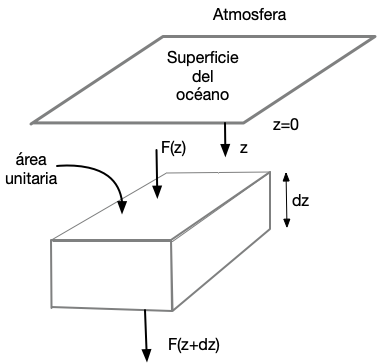
\includegraphics[width=0.50\textwidth]{figuras/COS_model.png}
\caption{Diagrama del ejercicio}
\label{COS_fig}
\end{center}
\end{figure}

\begin{equation}
\Delta F=F(z)-F(z+\mathrm{d}z)=F(z)-\left[ F(z)+\frac{\mathrm{d}F(z)}{\mathrm{d}z}\mathrm{d}z \right]=-\mathrm{d}F(z)
\end{equation}
Como el volumen de la losa es $1\cdot \mathrm{d}z$ 
\begin{equation}
\textrm{el flujo neto de COS en una unidad de volumen de la losa} =-\frac{\mathrm{d}F(z)}{\mathrm{d}z}
\label{flux_COS}
\end{equation}
Si $D$ coeficiente de difusi�n en remolino,
\begin{equation}
F(z)=-D\frac{\mathrm{d}C(z)}{\mathrm{d}z}
\label{dif_COS}
\end{equation}
donde $C(z)$ es la concentraci�n de COS a la distancia $z$ debajo de la superficie del oc�ano, y el signo negativo surge porque la difusi�n ocurre en la direcci�n opuesta a la del aumento de la concentraci�n. En el presente caso, la concentraci�n de COS es mayor en la superficie del oc�ano y disminuye hacia abajo; por lo tanto, el flujo de COS es descendente en el oc�ano. De las ecuaciones. (\ref{flux_COS}) y (\ref{dif_COS})
\begin{equation}
\textrm{el flujo neto de COS en una unidad de volumen de la losa} =D\frac{\mathrm{d}^2C(z)}{\mathrm{d}z^2}
\label{flux2_COS}
\end{equation}
\noindent Si $k$ es el coeficiente de tasa de primer orden para la destrucci�n qu�mica de COS en aguas marinas 

\begin{equation}
\textrm{tasa de destrucci�n de COS en una unidad de volumen de la losa} =kC(z)
\label{des_COS}
\end{equation}
\noindent En condiciones de estado estacionario, de las ecuaciones (\ref{flux2_COS}) y  (\ref{des_COS})
\begin{equation}
\frac{\mathrm{d}C(z)}{\mathrm{d}t}=D\frac{\mathrm{d}^2C(z)}{\mathrm{d}z^2}-kC(z)=0
\label{cc_COS}
\end{equation}
La soluci�n de la ecuaci�n~\ref{cc_COS} es
\begin{equation}
C(z)=C(0)\exp(-z/H)
\label{c_cos}
\end{equation}
\noindent donde H (una altura de escala) est� dada por
\begin{equation}
H=\left( \frac{D}{k}\right)^{1/2} =  \left( \frac{0.0050}{5.0\times10^{-6}}\right)=32 \metre
\label{H_COS}
\end{equation}

Ahora se pueden responder las tres preguntas:

\begin{enumerate}
\item Cuando $C(z)=C(0)/2$, tenemos de las ecuaciones (\ref{c_cos}) y  (\ref{H_COS}) 
\begin{equation*}
\frac{1}{2}=\exp\left(-\frac{z}{H} \right)=\exp\left( -\frac{z}{32}\right)
\end{equation*}
Por lo tanto, z = 22m
\item La densidad de la columna de COS en el oc�ano es la masa total de COS en una columna de unidad de �rea de secci�n transversal que se extiende desde la superficie hasta el fondo del oc�ano. Por lo tanto
\begin{eqnarray*}
\textrm{Densidad de columna de COS} &=& \int_{z=0}^\infty C(z)\,\mathrm{d}z \\
       &=&  \int_{z=0}^\infty C(0)\exp\left(-\frac{z}{H}\right)\,\mathrm{d}z  \\
       &=& C(0)H \\
       &=& (1.0\times10^{-11})\times 32 \\
       &=& 3.2\times10^{-10}\kilogrampersquaremetre 
\end{eqnarray*}
%
\item De la ecuaci�n de tiempo de vida de un compuesto $\tau=\frac{M}{F}$
donde $M$ es la cantidad de sustancia qu�mica en, digamos, la columna de secci�n transversal unitaria que consideramos anteriormente y $F$ es la salida (tasa de eliminaci�n m�s tasa de destrucci�n) de la sustancia qu�mica de la columna. Por lo tanto, la vida media de una mol�cula de COS en el oc�ano viene dada por:
\begin{eqnarray*}
\tau & = & \frac{C(0)H}{k\int_0^\infty C(z)\,\mathrm{d}z } \\
& =& \frac{C(0)H}{kC(0)H}  \\ 
& =& \frac{1}{k}  \\ 
&=& \frac{1}{5.0\times10^{-6} \per\second}\\
&=& 2.3  \textrm{ dias} 
\end{eqnarray*}
\end{enumerate}
\end{example}
\subsection{Tierra s�lida}\index{fuentes!tierra@tierra s�lida}
Los volcanes son la fuente geoqu�mica m�s importante de gases traza en al atm�sfera. Aunque son muy localizados y muy variables, cuando las emisiones volc�nicas son lanzadas a la estratosfera (o superior), pueden dispersarse r�pidamente por todo el mundo y tener largos tiempos de residencia (1 a 2 a�o). El polvo fino  llega a dar varias vueltas alrededor de la Tierra. Los aerosoles producidos a partir de los gases pueden permanecer en la estratosfera durante varios a�os. Esto, a su vez, da lugar a un enfriamiento medio global en la superficie de $\sim0.4\degreecelsius$ en el a�o siguiente a la erupci�n; este enfriamiento llega a desaparecer despu�s de $\sim$3 a�os a medida que disminuye el polvo en la atm�sfera. Adem�s de cenizas y part�culas de polvo, los volcanes emiten \ce{H2O}, \ce{CO2}, \ce{SO2}, \ce{H2S}, COS, \ce{CS2}, HCl, HF, HBr, \ce{CH4}, \ce{CH3Cl}, \ce{H2}, CO y varios metales pesados vol�tiles (p. ej., Hg). Las rocas son una fuente de  cantidades peque�as de ciertos gases y son las principales fuentes de los gases He, Ar y Rn en la atm�sfera. El helio se produce principalmente del decaimiento radiactivo del uranio-238 y torio-232- No se acumula en la atm�sfera debido a que es tan ligero que escapa de la exosfera\index{exosfera}. El arg�n se ha acumulado durante eones debido a la desintegraci�n radiactiva del potasio-40 de rocas.

Las rocas carbonatadas, como la piedra caliza, que se presenta principalmente como calcita (es decir, \ce{CaCO3}), contienen 100,000 veces m�s carbono que la atm�sfera, pero la mayor parte est� secuestrada. Sin embargo, las rocas carbonatadas y los sedimentos marinos participan en un ciclo de per�odo largo con el \ce{CO2} atmosf�rico como se muestra a continuaci�n. La erosi�n de la calcita por el \ce{CO2} disuelto en la lluvia y en aguas dulces (r�os y lagos) se puede representar por

\begin{footnotesize}
\begin{eqnarray}
\ce{CO2}(g) + \ce{H2O} &\rightleftarrows& \ce{CO2}(ac) + \ce{H2O}(l)  \label{eq_co2h2o}\\
\ce{2H2O}(l) +   \ce{CO2}(ac)&\rightleftarrows&   \ce{H3O^+}(ac) +  \ce{HCO3^-}(ac) \label{eq_co2}\\
\ce{CaCO3}(s) +   \ce{H3O^+}(ac) +  \ce{HCO3^-}(ac) &\rightleftarrows& \ce{Ca^{2+}}(ac) + \ce{2HCO3^-}(aq) + \ce{H2O}(l)\label{eq_caco3}\\\hline
\textrm{Neto:       }   \ce{CaCO3}(s) +\ce{CO2}(g) + \ce{H2O}(l)  &\rightleftarrows&\ce{Ca^{2+}}(ac) + \ce{2HCO3^-}(aq)  \label{eq_cca}
\end{eqnarray}
\end{footnotesize}

La reacci�n (\ref{eq_co2h2o}) representa el equilibrio entre el \ce{CO2} en el aire y en los r�os y lagos de agua dulce. En la reacci�n (\ref{eq_co2}), el \ce{CO2} recibe un \ce{OH^-}  del \ce{H2O} para formar el �cido muy d�bil (es decir, poco ionizado) \ce{HCO3^-} (el ion bicarbonato), y en la reacci�n (\ref{eq_caco3}) el \ce{H3O+} remueve \ce{CO3^{2-}} del \ce{CaCO3} para formar otro ion bicarbonato\index{bicarbonato}. La reacci�n directa de (\ref{eq_caco3}) representa la erosi�n de la calcita por el \ce{CO2}  disuelto en aguas dulces.

Los productos de la \gloss[word]{meteorizacion} en el lado derecho de la Reacci�n (\ref{eq_cca}) eventualmente ingresan a los oc�anos, donde se precipitan para formar nuevos sedimentos (lo contrario de la Reacci�n (\ref{eq_cca})). A trav�s del levantamiento de las regiones de la plataforma continental, la subducci�n de sedimentos marinos hacia el manto superior y la corteza inferior de la Tierra y las erupciones volc�nicas, estos productos eventualmente regresan a los sedimentos continentales, completando as� este ciclo geoqu�mico. Los tiempos de residencia del \ce{Ca^{2+}}(aq) y del \ce{HCO3^-}(aq) en los oc�anos son $\sim 8\times 10^5$ y $\sim7.5 \times 10^4$ a�os, respectivamente.

\begin{example}
Cuando el \ce{CO2} se disuelve en agua pura �que reacciones se producen?

\textbf{Respuesta:}

\begin{footnotesize}
\begin{eqnarray}
\ce{CO2}(g) + \ce{H2O} &\rightleftarrows& \ce{H2CO3}(ac) \\
\ce{H2CO3}(ac) + \ce{H2O}(l) &\rightleftarrows&  \ce{HCO3^-}(ac) + \ce{H3O^+}(ac) \\
 \ce{HCO3^-}(ac) + \ce{H2O}(l) &\rightleftarrows&  \ce{CO3^{-2}}(ac) + \ce{H3O^+}(ac) \\ \hline
 \textrm{Neto:         } \ce{CO2}(g) + 3\ce{H2O} &\rightleftarrows& \ce{CO3^{-2}}(ac) +2 \ce{H3O^+}(ac) 
 \end{eqnarray}
\end{footnotesize}
\end{example}

\subsection{Oc�anos}\index{fuentes!oceano@oc�ano}
La mayor�a de los gases que pasan de los oc�anos al aire se originan en procesos biol�gicos, que se analizan en la subsecci�n (\ref{subbio}). Adem�s, como vimos en la subsecci�n anterior, los oc�anos pueden participar en el ciclo de gases entre la Tierra s�lida y la atm�sfera. 

Los oc�anos son un enorme reservorio de aquellos gases que son apreciablemente solubles en agua. Los oc�anos pueden servir como fuente y sumidero de gases traza en la atm�sfera.

\subsection{Formaci�n in situ en la atm�sfera.}\index{atmosfera@atm�sfera!fuentes de contamiantes}

Las reacciones qu�micas en la atm�sfera son una fuente importante y un sumidero de muchos constituyentes traza. Los gases traza emitidos por la biosfera, la Tierra s�lida y los oc�anos generalmente se encuentran en un estado de oxidaci�n reducido (es decir, m�s bajo) (por ejemplo, C, N y S), pero cuando regresan a la superficie de la Tierra generalmente se encuentran en un estado de  mayor oxidaci�n.

Los procesos que producen estas transformaciones se pueden dividir en reacciones de fase gaseosa homog�nea, fase acuosa homog�nea y reacciones heterog�neas.

 \section{El esmog}\index{esmog}

 La contaminaci\'on ambiental se encuentra presente en nuestra vida y es producto de las actividades de la vida cotidiana tanto en las ciudades como en el campo. La principal causa de la contaminaci\'on en el aire es debido a la combusti\'on, y \'esta es de suma importancia para el ser humano. Cuando ocurre la combusti\'on perfecta o te\'orica, el carbono e hidr\'ogeno del combustible se combinan con el ox\'{\i}geno del aire desprendiendo calor, luz y generando bi\'oxido de carbono y vapor de agua. Sin embargo las impurezas del combustible, el mezclado imperfecto, la temperatura exterior afectan la combusti\'on gener�ndose impurezas tales como mon\'oxido de carbono, di\'oxido de azufre, \'oxidos de nitr\'ogeno, holl\'in y combustible no quemado ---todos ellos son contaminantes del aire.
 
 El esmog es la combinaci\'on de part\'{\i}culas de humo de fuentes industriales con neblina produciendo un color negro-amarillento cerca de la superficie (nieblumo)\index{esmog!nieblumo}. La combusti\'on de gasolina puede crear otro problema de contaminaci\'on conocido como ``esmog fotoqu\'{\i}mico''. Este se genera cuando los contaminantes primarios (\'oxidos de nitr\'ogeno y COV) interact\'uan bajo la influencia de la luz solar para producir una mezcla de cientos de sustancias t\'oxicas diferentes conocidas como contaminantes secundarios. Es una bruma marr\'on que contamina las ciudades. Puede hacer dif\'{\i}cil el respirar para algunas personas y reduce la visibilidad.

 \subsection{Europa}
En diciembre de 1930, una regi\'on altamente industrializada del Valle de Meuse, en B\'elgica, se cubri\'o durante 3 d\'{\i}as de una espesa niebla, por lo que cientos de personas enfermaron y 60 murieron ---m\'as de 10 veces el n\'umero normal.  

En Inglaterra durante 9 d\'{\i}as, en enero de 1931, murieron 592 personas --lo que nuevamente representaba un considerable incremento en la tasa de mortalidad. En 1948, en Donora, Pennsylvania, un peque\~no pueblo en donde hab\'{\i}a plantas qu\'{\i}micas y acerer\'{\i}as se cubri\'o por una niebla durante 4 d\'{\i}as,  enferm\'o casi la mitad de sus 14,000 habitantes. Murieron 20 personas. No fue hasta que una gran capa de niebla cubri\'o Londres en 1952 cuando se hizo totalmente evidente el siniestro potencial de la contaminaci\'on del aire. La niebla dur\'o desde el 5 de diciembre hasta el 8, y 10 d\'{\i}as despu\'es se supo que el n\'umero total de muertes en la regi\'on principal de Londres sobrepasaba en 4,000 al promedio. Las estad\'{\i}sticas indicaron que casi todos los que hab\'{\i}an muerto inesperadamente ten\'{\i}an antecedentes cl\'{\i}nicos de bronquitis, enfisema o trastornos card\'{\i}acos, y que las personas clasificadas en la \'ultima categor\'{\i}a, eran las m\'as vulnerables. Nuevamente, en enero de 1956, se produjeron 1,000 muertes m\'as debido a una extensa niebla.

 
 \subsection{Los Angeles}
En contraste con la contaminaci\'on en Londres los episodios de contaminaci\'on en Los Angeles y la Ciudad de M\'exico se dan en situaciones de cielos despejados con sistemas de alta presi\'on que limitan la dispersi\'on de contaminantes. En este caso las emisiones primarias de los procesos industriales, comerciales y del transporte reaccionan en la atm\'osfera generando nuevos contaminantes que afectan la salud de los seres humanos, animales, plantas  y afectando a los materiales.

\subsection{Clasificaci\'on de Contaminantes}

Los contaminantes atmosf\'ericos se pueden clasificar de diversas maneras, una de ellas es por su composici\'on:\index{contaminante!clasificaci\'on}

\begin{itemize}
\item \textbf{Org\'anicos} Contienen carbono, hidr\'ogeno (\ce{CH4}) y pueden incluir ox\'{\i}geno (HCHO), nitr\'ogeno (\ce{CH3NH2}), azufre (DMS).
\item \textbf{Inorg\'anicos} Compuestos de azufre (\ce{SO2}, \ce{H2S}), nitr\'ogeno (\ce{NO_$x$}), halogenados (CFC)\index{CFC}, metales pesados (As, Pb, Cd, etc)
\end{itemize}
Por su estado f\'{\i}sico:
\begin{itemize}
\item Gases y vapores
\item Part\'{\i}culas (s\'olidas y l\'{\i}quidas).
\end{itemize}

A su vez las part\'{\i}culas se pueden clasificar de acuerdo a con su tama\~no, como se muestra en el \textbf{Cuadro~\ref{part:1}} en p\'agina~\pageref{part:1}

Tambi\'en se puede categorizar los contaminantes por su origen de la siguiente  forma:\index{contaminante!primarios}\index{contaminante!secundario}
\begin{description}
\item[Primarios] Aquellos que son emitidos directamente
dentro de la atm\'osfera. Como lo son el mon\'oxido de nitr\'ogeno (NO), di\'oxido de azufre (\ce{ SO2}), el mon\'oxido de carbono (CO).
\item[Secundarios] Creados a trav\'es de reacciones y procesos en la
atm\'osfera. Como el ozono (\ce{O3}), tri\'oxido de azufre (\ce{SO3}) y el nitrato de
peroxiacilo (PAN)\index{PAN}.
\end{description}
\section{Contaminantes criterio}\index{contaminante!criterio}

De todos los contaminantes posibles existe un conjunto de ellos que se emplean para calificar la calidad del aire  y se les conoce como  \textit{contaminantes criterio}, los contaminantes criterio son seleccionados debido a que pueden provocar efectos a la salud y son los que se muestran en el  \textbf{Cuadro~\ref{contcrit}}.
\begin{table}[htb]
\caption{Contaminantes Criterio}
\label{contcrit}
\begin{center}
\begin{tabular}{ll}\hline
Mon\'oxido de carbono & CO\\
Di\'oxido de azufre & \ce{SO2}\\
\'Oxidos de nitr\'ogeno &NO$_x$\\
Ozono & \ce{O3}\\
Part\'{\i}culas & PST/\ce{PM10},\ce{PM_{2.5}}\\
Plomo& Pb\\ \hline
\end{tabular}
\end{center}
\end{table}

De todos los compuestos que se han presentado los hidrocarburos (COV)\index{COV} no son contaminantes criterio, pero se estudian muy de cerca por su rol en la producci�n de ozono:

\begin{center}
COVs $+$ NO$_x +$luz solar $\longrightarrow$ esmog fotoqu\'{\i}mico (\ce{O3}) 
\end{center}

\subsection{Mon\'oxido de carbono (CO)}
\index{CO}
Es gaseoso, inodoro e incoloro es resultado de la combusti\'on incompleta de los veh\'{\i}culos, el 70\% del CO proviene de los veh\'{\i}culos y presenta un perfil diurno, con concentraciones m\'aximas en horas pico de tr\'ansito.

\subsubsection{Efectos a la salud:}
\index{CO}
El CO se puede ligar a la sangre en lugar del di�xido de carbono (\ce{CO2}) por lo que puede ser asfixiante al reducir el ox�geno (\ce{O2}) transportado -- disminuye la actividad cerebral, incrementa la frecuencia card\'{\i}aca. Los efectos dependen del nivel de actividad.
\begin{equation}
\%\ce{COHb}  = 0.005[\ce{CO]}^{0.85}(\alpha t)^{0.63}
\end{equation}
Donde:

\begin{tabular}{r @{---}l}
$\%\ce{COHb} $ & Carboxihemoglobina en la sangre en por ciento de sa\-tu\-ra\-ci\'on.\\
$[\ce{CO}]$ &Concentraci\'on de CO en ppm\\
$\alpha$ & Coeficiente de actividad ( 0.94 sedentario, 3 trabajo pesado)\\
$t$ & tiempo de exposici\'on en minutos\\
\end{tabular}

Algunos efectos por la cantidad de CO en la sangre son los siguientes:
\begin{itemize}
\item 2.5\% se muestran algunos efectos ligeros.
\item 5\% Se notan efectos psicomotores.
\item 10\% Mareos y dolor de cabeza.
\item 50\% Mortal.
\end{itemize}

\subsubsection{Fuentes de exposici\'on:}
Intersecciones muy transitadas, vivir cerca de vialidades transitadas, fumar.
Se requieren de 3 a 4 horas para alcanzar niveles altos de concentraci\'on de COHb, y
se requieren de 3 a 4 horas para recobrarse de la exposici\'on.

\subsection{Compuestos de azufre}\index{azufre!compuestos}
Este contaminante puede producir, incluso a grandes distancias de la fuente de emisi�n, efectos adversos sobre la salud (tales como irritaci�n e inflamaci�n del sistema respiratorio, afecciones e insuficiencias pulmonares, alteraci�n del metabolismo de las prote�nas, dolor de cabeza o ansiedad), sobre la biodiversidad, los suelos y los ecosistemas acu�ticos y forestales (puede ocasionar da�os a la vegetaci�n, degradaci�n de la clorofila, reducci�n de la fotos�ntesis y la consiguiente p�rdida de especies) e incluso sobre las edificaciones, a trav�s de procesos de acidificaci�n, pues una vez emitido, reacciona con el vapor de agua y con otros elementos presentes en la atm�sfera, de modo que su oxidaci�n en el aire da lugar a la formaci�n de �cido sulf�rico.

Adem�s, tambi�n act�a como precursor de la formaci�n de sulfato am�nico, lo que incrementa los niveles de \ce{PM10} y \ce{PM_{2.5}}, con graves consecuencias igualmente sobre la salud.

\subsubsection{Fuentes de emisi�n del di�xido de azufre} Las principales fuentes de azufre en la atm�sfera son el uso de combustibles f�siles y las exhalaciones volc�nicas\index{volcan@volc�n}. El compuesto que principalmente se emite es el di�xido de azufre (\ce{SO2}). La fuente  \gloss[word]{antropica} principal es la quema de combustibles conteniendo azufre, el 85\% del total de emisiones proviene de esta fuente. Algunas industrias de la fundici\'on, la refinaci\'on, la minera --  tienen normas de emisi�n de este compuesto.

El contenido de azufre en los combustibles abarca el intervalo de 0.05 a 6\% en los combustibles l\'{\i}quidos y en el carb\'on. Cuando se queman se emite el di\'oxido de azufre (\ce{SO2}).
Produce lluvia \'acida\index{lluiva@lluvia �cida}, tambi\'en se condensa en part\'{\i}culas formando \ce{SO_4^=} durante el per\'{\i}odo de d\'{\i}as
\begin{itemize}
\item Exposici\'on a 1 ppm de \ce{SO2} por 15--20 min se observan cambios en el pulso y
respiraci\'on.
\item 0.3 ppm por 1--3 d\'{\i}as enfermedades cardio-respiratorias, muertes en Londres.\index{Londres}
\item 0.002 ppm por un a\~no, incrementa las admisiones al hospital.
\end{itemize}

\subsection{Compuestos de nitr�geno}
\index{nitrogeno@nitr�geno!compuestos de} 
En la atm�sfera se pueden encontrar formas oxidadas del nitr�geno 

NOx= NO + \ce{NO2},

NOy =NOx + \ce{NO3} + HONO + \ce{HNO3} + \ce{N2O5} + PAN

NOz = NOy -NOx

y las formas reducidas amon�aco\index{amoniaco@amon�aco} (\ce{NH3}), cianuro de hidr�geno (HCN)\index{cianuro}  y algunos hom�logos mayores como aminas alif�ticas\index{aminas!alifaticas@alif�ticas} y arom�ticas\index{aminas!aromaticas@arom�ticas}  \ce{RNH2}, RR'NH y RR'R''N y los n�tralos RCN, donde R, R' R'' = son grupos alquilos\index{grupo!alquilo}  o \gloss[word]{arilo}\index{grupo!arilo} .

\subsubsection{\'Oxidos de Nitr\'ogeno (NO$_x$)}
La suma de \ce{NO} + \ce{NO2} se refiere como NO$_x$, principalmente proviene de la combusti\'on:
\begin{description}
\item[NO$_x$ Termal] Cuando el \ce{N2}  y el \ce{O2} se calientan a altas temperaturas
($>400^\circ C$)
\item[NO$_x$ Combustible] Del nitr\'ogeno contenido en el combustible.
\end{description}
La emisiones de NO$_x$ son principalmente NO, \'este reacciona y forma el \ce{NO2} que absorbe la luz.
%\begin{eqnarray}
%\ce{NO2} + \textrm{hidrocarburos}&\longrightarrow&\textrm{esmog}\index{esmog}\\
%\ce{NO2}+ \ce{OH}\cdot &\longrightarrow&\ce{HNO3} \: \textrm{(Lluvia \'acida)} \index{lluiva@lluvia �cida}
%\end{eqnarray} 

\subsubsection{Control} En emisiones de fuentes estacionarias y en motores de veh\'{\i}culos. Reduciendo la temperatura de combusti\'on y con combustibles con bajo nitr�geno (N). Altas temperaturas disminuyen el mon�xido de carbono (CO) pero incrementan la emisi�n de  NO$_x$.

\subsection{Ozono (\ce{O3}) \label{o3_salud}}\index{ozono}
El ozono no se emite directamente a la atm\'osfera, se produce mediante una serie de reacciones que involucran a los \'oxidos de nitr\'ogeno, hidrocarburos y la luz solar ($h\nu$). El ozono posee dos efectos -- da\~nos a la salud y a los materiales.

Efectos del ozono en materiales:
\begin{itemize}
\item Reduce la vida \'util de llantas y hules.
\item Puede da\~nar a la vegetaci\'on (reduce la producci\'on agr\'{\i}cola)
\end{itemize}
Efectos del ozono en la salud:
\begin{itemize}
\item Irritaci\'on de ojos.
\item Constricci\'on del pecho, irritaci\'on en la garganta.
\item Altas concentraciones agravan las enfermedades respiratorias.
\end{itemize}
%Reacciones atmosf\'ericas que producen el ozono:
%\begin{eqnarray}
%\ce{NO2 + h\nu} &\longrightarrow& \ce{NO + O} \\
%\ce{O + O2 + M} &\longrightarrow& \ce{O3 + M}\\
% \ce{O3 + NO} &\longrightarrow& \ce{NO2 +  O2 }
%\end{eqnarray}
%
%Donde M es una mol\'ecula  (usualmente \ce{O2} o \ce{N2}). Las reacciones anteriores no explican las altas concentraciones de ozono observadas, existen otro conjunto de reacciones  con hidrocarburos las cuales producen radicales libres. Sea RH un hidrocarburo general entonces tenemos:
%
%\begin{eqnarray}
%\ce{RH + OH\cdot} &\longrightarrow& \ce{R\cdot}+ \ce{H2O}\\
%\ce{R\cdot }  +  \ce{O2} &\longrightarrow& \ce{RO2\cdot} \quad(\textrm{\footnotesize radical peroxialquil})\\
%\ce{RO2\cdot}  +\ce{ NO} &\longrightarrow& \ce{R\cdot} + \ce{NO2}
%\end{eqnarray}
La  formaci\'on de ozono depende de la disponibilidad del \ce{NO2}  y la destrucci\'on depende de la concentraci\'on del NO. Sin embargo en las ciudades el efecto global de las reacciones con hidrocarburos (COV) es convertir el \ce{NO} a \ce{NO2} por lo cual hace que se incremente la concentraci�n del \ce{O3}.

El control del ozono se da a trav\'es de controlar sus precursores, \'oxidos de nitr\'ogeno, y compuesto org\'anicos. Si el aire se encuentra ``atrapado'' por la
orograf\'{\i}a y condiciones meteorol\'ogicas como la inversi\'on t\'ermica, esto puede empeorar el problema como:

\begin{itemize}
\item Los Angeles
\item M\'exico D.F.
\item Grecia
\item Valle Fraser (frontera EU/Canada)
\end{itemize}

\paragraph{Nota sobre ozono}
\index{ozono!troposf\'erico}
\index{ozono!estratosf\'erico}
Existen dos diferentes zonas donde se encuentra el ozono, el troposf\'erico (nivel del
suelo) y el estratosf\'erico. En el \textbf{Cuadro~\ref{ozon:1}} se pueden observar las
caracter\'{\i}sticas y efectos que posee el ozono en las diferentes zonas.
\begin{table}[hbt]
\caption{Ozono en la atm\'osfera}
\label{ozon:1}
\begin{center}
{\footnotesize \begin{tabularx}{.8\textwidth}{X|X}
\textbf{Ozono Troposf\'erico}&\textbf{Ozono Estratosf\'erico}\\ \hline \hline
Localizado entre $0$--$10$ km& Localizado entre $15$--$35$ km\\
Contiene el $10$\% del ozono de la atm\'osfera&
Contiene el $90$\% del ozono de la atm\'osfera\\
Impacto da\~nino: efectos t\'oxicos en seres humanos y vegetaci\'on&
Rol ben\'efico: Act\'ua como escudo a la radiaci\'on UV\\
T\'opicos actuales: -- Episodios de alta concentraci\'on en superficie en ciudades.&
T\'opicos actuales: Disminuci\'on en la concentraci\'on. Hoyo de ozono en la
primavera ant\'artica\\\hline
\end{tabularx}}
\end{center}
\end{table}

\subsection{Part\'{\i}culas}
Se define como part\'{\i}culas a cualquier material disperso, s\'olido,
l\'{\i}quido, en el cual sus part\'{\i}culas individuales son mayores que una 
mo\-l\'e\-cu\-la pero menores a $500\mu m$

En el \textbf{Cuadro \ref{part:1}}  se enlistan en diferentes categor\'{\i}as las part\'{\i}culas:
\begin{table}[h!]
\caption{Definici\'on de las part\'{\i}culas suspendidas en el aire}
\label{part:1}
\begin{center}
{\scriptsize \begin{tabularx}{\linewidth}{>{\setlength{\hsize}{.35\hsize}}X%
>{\setlength{\hsize}{1.65\hsize}}X} \hline
{\footnotesize Part\'{\i}culas} & Cualquier material, excepto agua no combinada, que
existe en estado s\'olido o l\'{\i}quido en la atm\'osfera o en una corriente de gas
en condiciones normales.\\
{\footnotesize Aerosol} & Una dispersi\'on de part\'{\i}culas microsc\'opicas, s\'olidas o
l\'{\i}quidas. \\
{\footnotesize  Polvo} & Part\'{\i}culas s\'olidas de un tama\~no mayor que el coloidal, capaces
 de estar en suspensi\'on temporal en el aire.\\
{\footnotesize Ceniza fin}a& Part\'{\i}culas de ceniza finamente divididas arrastradas
por el gas de combusti\'on. Las part\'{\i}culas pueden contener combustible no
quemado\\ 
{\footnotesize  Niebla} &Aerosol visible.\\
{\footnotesize Vapores}& Part\'{\i}culas formadas por la condensaci\'on, sublimaci\'on,
o reacci\'on qu\'{\i}mica, predominantemente mayores de 1$\mu m$ (humo de
tabaco).\\
{\footnotesize Neblina} & Dispersi\'on de peque\~nas gotas de l\'{\i}quido de suficiente tama\~no como
para caer.\\
 {\footnotesize Part\'{\i}cula}& Masa discreta de materia s\'olida o l\'{\i}quida.\\
{\footnotesize Humo}& Part\'{\i}culas peque\~nas arrastradas por los gases, que resultan
dela combusti\'on.\\
{\footnotesize Holl\'{\i}n}& Una aglomeraci\'on de part\'{\i}culas de carb\'on.\\ \hline
\end{tabularx}}
\end{center}
\end{table}
\subsection{Plomo (\ce{Pb})}
Hasta 1980 proven\'{\i}a principalmente de los autom\'oviles que conten\'{\i}an en sus
combustibles el tetraetilo de plomo \ce{(C2H5)_4Pb} teniendo 1.1 g por gal\'on. 
\subsubsection{Efectos en la salud}
El plomo es emitido como sales de plomo depositadas cerca de las v\'{\i}as de tr\'ansito, las
part\'{\i}culas son transportadas a las casas por la pisadas, se resuspenden en el
interior y son inhaladas.

Otras v\'{\i}as de exposici\'on son plomo en el agua por fugas en tuber\'{\i}as o
soldaduras de plomo,  o es ingerido de pinturas o suelo.

El plomo llega a la sangre y reemplaza al hierro en ni\~nos, lo cual puede resultar en
discapacidad para aprender o da\~no severo al cerebro.

De 20 a 50$\mu$g de plomo en un decilitro de sangre provoca da\~nos a la salud.

\subsubsection{Visibilidad}

La radiaci\'on se dispersa efectivamente con objetos de tama\~no similar a la longitud
de onda de la radiaci\'on. La luz visible posee una longitud de onda de 0.38 a 0.70
$\mu m$. Part\'{\i}culas en la atm\'osfera con este tama\~no pueden dispersar la luz y
con ello causar una reducci\'on en la visibilidad. Esto se puede notar en distancias
cortas con altas concentraciones o en grandes distancia con bajas concentraciones.
\paragraph{Nota sobre las part\'{\i}culas}
Cuando se especific\'o la norma de part�culas, \'estas se regular\'on como Part\'{\i}culas Suspendidas Totales (PST) \index{PST}. Esta fue la medida del material particulado en el aire.\index{material particulado}

En 1987 en EU la norma cambi\'o a PM10 -- toda part\'{\i}cula menor a 10$\mu m$ en di\'ametro.

En 1997, otra norma de part\'{\i}culas se adicion\'o --- \ce{PM_{2.5}} -- toda part\'{\i}cula menor a $2.5\mu m$ en di\'ametro.

\section{Compuestos t\'oxicos en el aire}
\normalsize
El t\'ermino de \emph{compuestos t\'oxicos} se refiere a cualquier substancia  encontrada en el aire.para prop\'ositos de regulaci\'on, la Agencia de Protecci\'on Ambiental de los EU se refiere a dos clases de contaminantes: los contaminantes criterio y t\'oxicos ambientales. Existen normas nacionales de contaminantes criterio por que esos contaminantes se liberan en grandes cantidades por una gran variedad de fuentes y presentan un riesgo a la salud y bienestar humano en grandes regiones. El di\'oxido de azufre, el di\'oxido de nitr\'ogeno, el mon\'oxido de carbono,  part\'{\i}culas, ozono  y plomo son los contaminantes criterio. Los t\'oxicos del aire incluyen varias sustancias emitidas al aire. Existe una lista de 189 contaminantes, algunos listados en el \textbf{Cuadro~\ref{airtox}}, incluyendo en esta lista est\'an las substancias identificadas como cancerog\'enicas, mutag\'enicas o toxinas de reproducci\'on. Los m\'etodos de an\'alisis de riesgos que se siguen aplican a cualquier sustancia t\'oxica encontrada en el aire, pero los ejemplos num\'ericos se concentrar\'an en los compuestos de la lista del \textbf{Cuadro~\ref{airtox}}.

 \begin{table}[htdp]
\caption{Contaminantes T\'oxicos}
\begin{scriptsize}
\tablefirsthead{  \hline {\bf CAS} & {\bf Compuesto} &{\bf  CAS} &{\bf Compuesto}\\}
\begin{supertabular}{| p{0.10\textwidth}p{0.35\textwidth}p{0.10\textwidth}p{0.35\textwidth} |}\hline%
75070 & Acetaldeh\'{\i}do &133904 & Cloranfen \\
60355 & Acetamina  & 57749 & Clordano\\
75058 & Acetonitrilo & 7782505 & Cloro \\
98862 & Acetofenona & 79118 & Ac. clorac\'etico\\
53963 & 2-Acetilaminofluoreno & 532274 & 2-Cloracetafenona\\
107028 & Acroleina & 108907 & Clorobenceno\\
79061 & Acrilamina & 510156 & Clorobencilato\\
79107 & Ac. acr\'{\i}lico & 67663 & Cloroformo\\
107131 & Acrilonitrilo & 107302 & Clorometil metil eter\\
107051 & Alil cloruro & 126998 & Cloropreno \\
92671 & 4-aminobifenil & 1319773 & Cresoles (isomeros y mezclas)\\
62533 & Anilina &9587 &\emph{o}-Cresol\\
90040 & \emph{o}-Anisidina & 108394 &\emph{m}-Cresol \\
1332214 & Asbestos & 106445 &\emph{p}-Cresol \\
71432 & Benceno (incluyendo& 98828 &Cumeno \\
            & benceno de gasolina) & 94757 &2,4-diclorofenoxiac\'etico,  \\
92875 & Bencidina &  &sales y esteres\\
98077 & Benzotricloro & 3547044 & DDE\\
100447 & Cloruro de Bencilo & 334883 &  Diazometano\\
92524 & Bifenil & 132649 & Dibenzofuranos\\
117817 & Bis(2-etilhexil) ftalato (DEHP) & 96128 & 1,2-Dibromo- 3- cloropropano\\
542881& Bis(clorometil) eter &8742&Dibutilftalato\\
75252 & Bromformo &106467&1,4- Dicloro benceno (p) \\
106990 &1,3-Butadieno &91941& 3,3-Diclorobencidine \\
156627 & Cianamida de calcio &111444&Dicloroetil eter (bis(2-cloroetil)eter)\\
105602& Caprolactama& 542756 &1,3-Dicloropropeno\\ 
133062 & Captan & 62737 & Diclorvos (DDVP)\\
63252 & Carbaril &111422& Dietanolamina\\
75150 & Disulfuro de carbono & 121697 & N,N-Dietilanilina (NN-Dimetilanilina) \\
56235 & Tetracloruro de Carbono &64675&Sulfato de dietilo\\
463581 & Sulfuro de Carbonilo  &110543&Hexano\\
120809 & Catecol & 302012&Hidrazina \\
119904 & 3,3-Dimetoxybencidina &7647010&  \'Acido Hidrocl\'orico\\
60117 & Dimetil ainoazoenceno&7664393& Fluoruro de hidr\'ogeno\\
119937 & 1,3-Dimetil bencidine & &(\'acido fluorh\'{\i}drico)\\
79447 & Clouro de Dimetil cabamol&123319&Hidroquinona\\
  68122 & Dimetil formamida &78591&Isoforona\\
  57147 & 1,2-Dimetil hidracina & 58899&Lindano ( todos sus is\'omeros) \\
  131113&  Dimetil ftalato &108316&Anh\'{\i}drico mal\'eico \\
  77781 &Dimetil sulfato &67561&Metanol \\
  534521& 4,6-Dinitro-o-cresol y sales & 72435&Metoxiclor \\
  51285 & 2,4- Dinitrofenol & 74839 & Bromuro de metilo (bromometano)\\
  121142 & 2,4- Dinitrotolueno & 74873& Cloruro de metilo \\
  123911 & 1,4 Dioxano (1,4-oxido de dietileno) &71556&Metil clororformo (1,1,1-tricloroeteno)\\
  122667 & 1,2-Difenilhidrazina &78933&Metil etil cetona (2-butanona) \\
  106898 & Epicloridina (1-cloro 2,3-epoxipropano)&60344 &Metil hidrazina\\
  106887 & 1,2-Epoxibutano &74884&Ioduro de metilo (iodometano)\\
  140885 & Etil acrilato &51796 &Carbamoato de etilo (uretano) \\
  100414 & Etil benceno &  &\\\hline
\end{supertabular}
\end{scriptsize}
\label{airtox}
\end{table}%


\subsection{Efectos a la salud}
Los efectos a la salud relacionados con la exposici\'on a los compuestos t\'oxicos pueden variar ampliamente. Un efecto espec\'{\i}fico en la salud usualmente se relaciona a un intervalo de niveles de exposici\'on. El \textbf{Cuadro~\ref{efectos}} lista algunos contaminantes y sus efectos asociados con la salud.
\index{contaminacion@contaminaci\'on!efectos a la salud}
 \begin{table}[htdp]
\caption{Efectos a la salud de algunos contaminantes}
\begin{center}
{\small
\begin{tabular}{|l|l|}\hline
{\bf Contaminante} &{\bf  Efectos a la salud}\\\hline
Ozono   & Problemas en el tracto respiratorio como la dificultad de respirar,  \\
               &  reducci\'onde la funci\'on respiratoria, a la resistencia a la infecci\'on, \\
               & asma, irritaci\'on de ojos, congesti\'on,  y posible envejecimiento \\
               & del tejido pulmonar.\\ \index{ozono!efectos a la salud}
Part\'{\i}culas  & Irritaci\'on de ojos y garganta, bronquitis, da\~no al pulm\'on\\
               & reducci\'on de la visibilidad.\\ \index{material particulado} \index{particulas@part�culas!efectos a la salud}
CO        & Incapacidad de la sangre para transportar ox\'{\i}geno; afectaci\'on\\
              & a los sistemas cardiovascular, nervioso y pulmonar\\ \index{monoxido@mon\'oxido!de carbono!efectos a la salud}
\ce{SO2}& Problemas en el tracto respiratorio, da\~no permanente a los\\
             & tejidos del pulm\'on\\  \index{SO2@\ce{SO2}!efectos a la salud}   
Plomo  & Retardo y da\~no cerebral, especialmente en ni\~nos\\\index{plomo}
\ce{NO2}& Enfermedades respiratorias y da\~no al pulm\'on\\ \index{no2@\ce{NO2}!efectos a la salud}
Asbesto & Variedad de enfermedades de pulm\'on, particularmente c\'ancer \\\index{asbesto!efectos a la salud}
Berilio  & Primeramente da\~no al pulm\'on, aunque tambi\'en da\~na al h\'{\i}gado,\\ \index{berilio!efectos a la salud}
             &  bazo, ri\~nones y gl\'andulas linf\'aticas.\\ \index{higado@h\'{\i}gado}
Mercurio& Varias \'areas del cerebro como tambi\'en hay afectaci\'on en los \\
                & ri\~nones e intestinos\\ \index{mercurio!efectos a la salud}
Cloruro de vinilo& C\'ancer de pulm\'on e h\'{\i}gado\\ \index{vinilo! cloruro de}
Ars\'enico & C\'ancer\\ \index{arsenico@ars\'enico!efectos a la salud}
Radion\'ucleos& C\'ancer\\ \index{radionucleos@radion\'ucleos!efectos a la salud}
Benceno & Leucemia\\ \index{benceno!efectos a la salud}
Emisiones de coke & C\'ancer en vias respiratorias\\ \hline
\end{tabular}}
\end{center}
\label{efectos}
\end{table}%

\clearpage

 

\chapter{Fisicoqu\'{\i}mica en procesos atmosf\'ericos}

En la naturaleza se pueden identificar muchos de los procesos que se han revisado hasta ahora, como lo es el equilibrio qu\'{\i}mico, donde la cantidad de producto depende de los reactivos, la espontaneidad del proceso, las caracter\'{\i}sticas de las fases, entre otros. De este tipo de equilibrios dependen la acidez, la partici\'on de concentraciones entre la fase gaseosa y la fase l\'{\i}quida y la solubilidad que continuaci\'on se describen.  

 \section{Solubilidad}\index{solubilidad}
 
Una soluci\'on es una mezcla homog\'enea de sustancias. Cuando el az\'ucar se disuelve en agua, una mezcla homog\'enea o soluci\'on se forma. El componente que presenta la mayor cantidad en la mezcla determina la fase o el estado (s\'olido, l\'{\i}quido, o gas) de la soluci\'on es el \emph{\gloss[word]{solvente}}.\index{solvente} El otro componente es conocido como \emph{\gloss[word]{soluto}}.\index{soluto} Si se emplea agua como solvente, se dice que la soluci\'on es acuosa (ac).\index{solucion@soluci\'on!acuosa} Ejemplos de soluciones comunes se muestran en el \textbf{Cuadro~\ref{soluciones}}.

 \begin{table}
\caption{ Ejemplos de soluciones}
{\footnotesize
 \begin{tabular}{llll}
Soluci\'on & Estado de la  & Estado del & Estado del(os) \\
           & Soluci\'on    & Solvente   & Soluto(s) \\\hline
Atm\'osfera terrestre & Gas & Gas \ce{N2} & Gas-\ce{O2}, Ar, \ce{CO2}\\
Agua de Oceano & L\'{\i}quido & L\'{\i}quido-\ce{H2O} & S\'olido-sales-NaCl\\
               &              &                 & gas--\ce{O2}, \ce{CO2}\\
Joyer\'{\i}a de oro &     S\'olida & S\'olido--Au    & S\'olido--Ag,Cu\\
Agua de acuario&     Liquida  & L\'{\i}quido--\ce{H2O} & Gas--\ce{O2}, \ce{CO2}\\
Di\'oxido de carbono en hielo &S\'olido & S\'olido--hielo &Gas--\ce{CO2}\\\hline
\end{tabular}}
\label{soluciones}
\end{table}

\subsection{Equilibrio acuoso}
\index{equilibrio!acuoso}

Hemos revisado con anterioridad los principios b\'asicos del equilibrio qu\'{\i}mico. Ahora aplicaremos estos principios al equilibrio ionico en soluciones acuosas.

Como punto de partida consideremos, ls disoluci\'on del sulfato de plata en agua (\ce{Ag2SO4})
\reaction{Ag2SO4 <=> 2Ag+(ac) + SO4^2-(ac)}
 
La constante de equilibrio para esta reacci\'on es:\\[2pt]

\hskip 3cm $K_{ps} = $ [\ce{Ag+(ac)}]$^2$[\ce{SO4^2-(ac)}] $=$1.4$\times10^{-5}$\\[2pt]

Si C son las moles de sulfato de plata en agua,  C moles de sulfato de plata se disuelven en 1 L de agua para producir 2C moles de i\'on plata (\ce{2Ag+}) y C moles de i\'on sulfato (\ce{SO4^2-}). As\'{\i}, $K_{ps}=$1.4$\times10^{-5} = C^3$ o $C=$ 0.0241 M. Por lo tanto, s\'olo 0.0241 moles de sulfato de plata se disuelven en 1L de agua.

Como $K_{ps}$ es el producto de las concentraciones de los iones, se le llama \emph{constante producto de solubilidad} (por eso el sub\'{\i}ndice ''ps``). El producto de solubilidad se usa generalmente para sustancia con bajas solubilidades. \index{producto!de solubilidad}

Los productos de solubilidad muy bajos se miden el\'ectricamente y esos valores se reportan en las tablas. Generalmente se listan los productos de solubilidad de sustancias poco solubles o parcialmente insolubles. Si la $K_{ps}$ es muy baja, se considera una sustancia \emph{insoluble}\index{insoluble} (en agua). En el caso de sustancias con solubilidad moderada o alta (como el NaCl o NaOH), no es \'util el empleo de los productos de solubilidad. Por que en lugar de definir  la constante de equilibrio en t\'erminos de concentraci\'on tendremos que definirla en t\'erminos de la \emph{actividad} de las sustancias.\index{actividad}

\begin{table}
\caption{Solubilidades en agua de algunos compuestos}
\hskip 0.5in\begin{tabular}{lll}\hline
Iones Negativos & Iones Positivos & Solubilidad\\
(aniones) & (cationes) & \\\hline
Todos               & \ce{Li+}, \ce{Na+}, K$^+$, Rb$^+$, Cs$^+$, Fr$^+$ & Soluble\\
Todos               & \ce{H+}             & Soluble\\
Todos               & \ce{NH4+} (amonio)  & Soluble\\
\ce{NO3-} nitrato   & Todos               & Soluble \\ 
\ce{CH3COO-} acetato& Todos               & Soluble\\
\ce{SO4^2-} sulfato & \ce{Ba^2+}, \ce{Sr^2+}, \ce{Pb^2+},\ce{Ca^2+} & Poco soluble\\
                    & Todos los dem\'as   & Soluble\\\hline 
\end{tabular}
\end{table}

 \subsection{Solubilidad de gases en agua}

 Algebr\'aicamente, podemos expresar las propiedades de la soluci\'on  diluida ideal mediante las siguientes ecuaciones:
\begin{eqnarray}
 p_1&= &x_1p_1^\circ\label{raoult}\\
 p_j&=& K_jx_j
 \label{henry}
 \end{eqnarray}
 
 Donde el sub\'{\i}ndice denota cualquiera de los solutos y el sub\'{\i}ndice uno denota el solvente. Todas las soluciones reales se aproximan al comportamiento descrito por las ecuaciones~\ref{raoult} y \ref{henry}, siempre y cuando  la soluci\'on est\'e suficientemente dilu\'{\i}da. Lo mismo es v\'alido si est\'an presentes varios solutos, pero la soluci\'on debe estar diluida en todos; cada soluto tiene un valor diferente de $K_j$.
 
 La Ley de \gloss[Word]{henry}, ecuaci\'on \ref{henry},  \index{Henry@\textbf{Henry}!ley de} relaciona la presi\'on parcial del soluto en la fase vapor con la fracci\'on molar del soluto en la soluci\'on a temperatura constante. Enfocando la relaci\'on desde otro punto de vista, la ley de Henry relaciona la fracci\'on molar en el equilibrio, solubilidad de \emph{j} en la soluci\'on, con la presi\'on parcial de \emph{j} en el vapor:
 
 \begin{equation}
x_j=\frac{1}{K_j}p_j
\label{henry2}
\end{equation}

La ecuaci\'on~\ref{henry2} expresa que la solubilidad $x_j$ de un constituyente vol\'atil es proporcional a la presi\'on parcial del mismo en la fase gaseosa en equilibrio con el l\'{\i}quido. La ecuaci\'on~\ref{henry2} se emplea para correlacionar los datos de solubilidad de gases en l\'{\i}quidos. Si el solvente y el gas no reaccionan qu\'{\i}micamente, la solubilidad de gases en l\'{\i}quidos es peque\~na, por lo general, de modo que se cumple la condici\'on de diluci\'on. 

\section{Lluvia \'acida}
\index{lluvia!acida@\'acida}

\subsection{Historia de la lluvia \'acida}
En el siglo XIX, la gente comenz\'o a darse cuenta de que la suciedad expulsada por las chimeneas de las viviendas y f\'abricas estaba ocasionando la contaminaci\'on de la lluvia. En \'epocas anteriores, la gente se hab\'{\i}a quejado del desagradable ambiente generado por el humo de las chimeneas. La lluvia \'acida puede producirse de forma natural. Los volcanes, las turberas y las plantas en descomposici\'on desprenden di\'oxido de azufre.

\begin{tabular}{cl}
1692 & Rob Boyle\\
     & En su libro ``General History of the Air''\\
     & incluye discusiones de ``Esp\'{\i}ritus nitrosos o sulfuros salinos''\\
1872 & Robert Angus Smith\\
     & En el libro ``The beginning of Chemical Climatology'' describi\'o \\
     & la importancia de las fuentes de combusti\'on de carb\'on en la precipi-\\
     & ta\-ci\-\'on m\'etodos de muestreo, da\~no a plantas y materiales.
\end{tabular}

La absorci\'on de \ce{CO2} en el agua de lluvia cambia el $p$H.  Para observar esto podemos aplicar los conocimientos anteriores. La solubilidad del \ce{CO2} en agua viene dada por:

\reaction{CO2_{(g)} + H2O <=> H2CO3_{(ac)}}

Para el equilibrio del \ce{CO2} con el \ce{H2O}, empleamos la constante de Henry ($H$)\index{Henry@\textbf{Henry}!constante} y la presi\'on parcial del \ce{CO2} ($P_{CO_2}$) y obtenemos la concentraci\'on del \'acido carb\'onico (\ce{H2CO3}):
\begin{equation}
[\ce{CO2.H2O}] =P_{\ce{CO2}}H \label{eq1}
\end{equation}

Como hemos visto el \'acido carb\'onico es un \'acido \emph{polipr\'otico}:

\reaction{H2CO3_{(ac)} + H2O_{(l)} <=> HCO3^-_{(ac)} + H3O^+_{(ac)}}
\reaction{HCO3^-_{(ac)} + H2O_{(l)} <=> CO3^{-2}_{(ac)} + H3O^+_{(ac)}}
con las constantes de disociaci\'on  a 25\celsius de $K_a=4.2\times10^{-7}$ y $K_{a2}=5.0\times10^{-11}$. Por lo tanto:
\begin{eqnarray}
\frac{[\ce{H3O+}][\ce{HCO3^-_{(ac)}}]}{[\ce{H2CO3_{(ac)}}]}&=K_{a1}=&4.2\times10^{-7}\label{ec1}\\
\frac{[\ce{H3O+_{(ac)}}][\ce{CO3^{-2}_{(ac)}}]}{[\ce{HCO3^-_{(ac)}}]}&=K_{a2}=&5.0\times10^{-11}\label{ec2}
\end{eqnarray}

Ahora calculemos la concentraci\'on de \ce{H3O+(ac)}, \ce{H2CO3(ac)}, \ce{HCO3^-(ac)}, \\  \ce{OH-}(ac), y \ce{CO3^{-2}(ac)} cuando el \ce{CO2} de la atm\'osfera se disuelve en agua pura de lluvia, dado que la solubilidad del \ce{CO2} en agua es $1.0\times10^{-5}$M a 25$^\circ C$ y 1 atm.  Como se tienen cinco inc\'ognitas se requieren de cinco ecuaciones  para resolver este problema y hasta hora tenemos dos ecuaciones~\ref{ec1} y \ref{ec2}. Las otras tres ecuaciones son dadas por la constante del producto i\'onico del agua ($K_w$):
\begin{equation}
[\ce{H3O+_{(ac)}}][\ce{OH-_{(ac)}}]=K_w=1.0\times10^{-14} \label{ec3}
\end{equation}
del balance de masa
\begin{equation}
[\ce{H2CO3}]\textrm{\footnotesize inicial} = 1.0\times10^{-5} M =
[\ce{H2CO3_{(ac)}}] +[\ce{HCO3-}]+[\ce{CO3^{-2}}]
\label{ec4}
\end{equation}
y la reacci\'on de balanceo de cargas:$$[\ce{H3O+}]=\sum n[x^{N-}]$$
\begin{equation}
[\ce{H3O+(ac)}]= [\ce{HCO3^-(ac)}] +2[\ce{CO3^{-2}(ac)}]+[\ce{OH^-(ac)}]
\label{ec5}
\end{equation}

Donde $1.0\times10^{-5}M$ en la Ec.~\ref{ec4} sigue el hecho de que por cada mol de \ce{CO2} disuelto en agua una mol  de \ce{H2CO3} se forma  (\ce{CO2 + H2O <=> H2CO3}) y el coeficiente 2 en la Ec.~\ref{ec5}  permite dos unidades negativas de carga por cada \ce{CO3^2-}.


Despejando el \ce{HCO3-} de la ecuaci\'on~\ref{ec1}  y sustituyendo el [\ce{CO2.H2O}] a partir de la ecuaci\'on~\ref{eq1} tenemos:

\begin{equation}
[\ce{HCO3-}]=\frac{k_1[\ce{CO2.H2O}]}{[\ce{H+}]}  = \frac{k_1H P_{\ce{CO2}}}{[\ce{H+}]}
\label{ec6}
\end{equation}

De la ecuaci\'on~\ref{ec2} despejamos el \ce{CO3^{-2}} 

\begin{equation}
[\ce{CO3^{-2}}]= \frac{k_2[\ce{HCO3-}]}{[\ce{H+}]}= \frac{k_1k_2HP_{\ce{CO2}}}{[\ce{H+}]^2}
\label{ec7}
\end{equation}

Se desea saber cual es el p$H$ del agua en equilibrio en la atm\'osfera donde se tiene  una  presi\'on parcial de \ce{CO2} ($P_{\ce{CO2}}$), as\'{\i} sustituimos en la ecuaci\'on~\ref{ec5} las ecuaciones \ref{ec6} y \ref{ec7}.

La concentraci\'on del \ce{OH-} la obtenemos de la constante de disociaci\'on del agua $K_w$ y tenemos que,
$K_w = [\ce{H3O+}][\ce{OH-}]$ despejando $[\ce{OH-}]$ de la ecuaci\'on~\ref{ec3} y sustituyendo esto en la ecuaci\'on~\ref{ec5} tenemos:

\begin{equation}
[\ce{H+}]=\frac{k_1H P_{\ce{CO2}}}{[\ce{H+}]} + 2 \frac{k_1k_2HP_{\ce{CO2}}} {[\ce{H+}]^2}+\frac{K_w}{[\ce{H+}]}
\end{equation}

Rearreglando obtenemos:

\begin{equation}
[\ce{H+}]^3 - (K_w +k_1HP_{\ce{CO2}})[\ce{H+}] - 2Hk_1k_2P_{\ce{CO2}}
\end{equation}

para una presi\'on parcial $P_{CO_2} = 380\times10^{-6}$ atm se obtiene a partir de resolver la ecuaci\'on c\'ubica: [\ce{H+}]=10$^{-5.6}$ entonces el p$H$= 5.6
\\

Para el caso del \ce{NH3}
$$\ce{NH3_{ac} <=> NH4^+ + OH^-}$$

Entonces:
\begin{equation*}
H_{\ce{NH3}} =\frac{ [\ce{NH_{3(ac)}}]} { P_{\ce{NH3}}} = 5.8\times10^1\frac{M}{atm}
\end{equation*}

\begin{equation*}
k =\frac {[\ce{NH4^+}][OH^-]} {[\ce{NH_{3(ac)}}]} = 5.6\times10^{-10}
\end{equation*}

\begin{equation*}
\ce{NH4^+} = \frac{k_1H_{\ce{NH3}}P_{\ce{NH3}}\cdot [H^+]} { Kw} 
\end{equation*}

\begin{equation*}
[H^+] + [\ce{NH4+}] = [OH^-] + [\ce{HCO3-}] +2[\ce{CO3^2-}]
\end{equation*}

Para el caso del \ce{SO2}


\begin{equation*}
[\ce{SO2}\cdot\ce{H2O}] = H_{\ce{SO2}} P_{\ce{SO2}}
\end{equation*} 
\begin{equation*}
H_{\ce{SO2}} =\frac{ [\ce{SO2}\cdot\ce{H2O}]} { P_{\ce{SO2}}} = 1.2\frac{\textrm{M}}{\textrm{atm}}
\end{equation*}

\begin{equation*}
k'_1 = \frac{[\ce{H+}][\ce{HSO3^-]}} {[\ce{H2SO3}]} = 1.71\times10^{-2}
\end{equation*}

\begin{equation*}
k'_2 = \frac{[H^+] [\ce{SO3^{2-}}]}{[\ce{HSO3-}]} = 5.98\times10^{-8}
\end{equation*}

\begin{equation*}
[H^+] = [OH^-] + [\ce{HSO3-}] +2[\ce{SO3^{-2}}]
\end{equation*}

Despejando de k$'_1$  el [\ce{HSO3-}], de  k$'_2$  el [\ce{SO3^{-2}}]

\begin{equation*}
[\ce{HSO3-}] =\frac{ k_1[\ce{H2SO3}]} {[H^+]} 
\end{equation*}

\begin{equation*}
[\ce{HSO3-}]= \frac{k_1 H_{\ce{H2SO3}}P_{\ce{H2SO3}}} {[\ce{H+}]}
\end{equation*}

\begin{equation*}
[\ce{SO3^{2-}}] =\frac{k_2[\ce{HSO3-}]} {[\ce{H+}]} 
\end{equation*}

\begin{equation*}
[\ce{SO3^{2-}}]=\frac{k'_1k'_2H_{\ce{H2SO3}}P_{\ce{H2SO}}} {[H^+]}
\end{equation*}

Juntando los tres compuestos obtenemos:

\begin{equation*}
[H^+] + [\ce{NH4+}] = [\ce{OH-}]+[\ce{HCO3-}]+2[\ce{CO3^{2-}}]+[\ce{HSO3-}]+2[\ce{SO^{2-}}]
\end{equation*}

 \begin{equation*}
\begin{split}
[\ce{H+}] + \frac{kH_{\ce{NH3}}P_{\ce{NH3}}}{[\ce{OH-}]} &= [\ce{OH-}] + \frac{k_1H_{\ce{CO2}}P_{\ce{CO2}}}{[\ce{H+}]} +\frac{2k_1k_2H_{\ce{CO2}}P_{\ce{CO2}}}{[\ce{H+}]^2} + \\
&\quad\frac{k'_1H_{\ce{SO2}}P_{\ce{SO2}}} {[\ce{H+}]} + \frac{2k'_1k'_2H_{\ce{SO2}}P_{\ce{SO2}}}{[\ce{H+}]^2}
\end{split}
\end{equation*}

sustituyendo el [\ce{OH-}]  por  $\frac{K_w}{[\ce{H+}]} $ queda: 
 \begin{equation*}
\begin{split}
[H^+] + \frac{kH_{\ce{NH3}}P_{\ce{NH3}}[H^+]}{Kw} &= \frac{Kw}{[H^+]} + \frac{k_1H_{\ce{CO2}}P_{\ce{CO2}}}{[H^+]} +\frac{2k_1k_2H_{\ce{CO2}}P_{\ce{CO2}}}{[H^+]^2} +\\ &\quad\frac{k'_1H_{\ce{SO2}}P_{\ce{SO2}}} {[H^+]} + \frac{2k'_1k'_2H_{\ce{SO2}}P_{\ce{SO2}}}{[H^+]^2}
\end{split}
\end{equation*}

\section{Termodin\'amica en la atm\'osfera.}

Si se desea conocer en la atm\'osfera si  el aire caliente se desplaza hacia arriba o hacia abajo, o identificar 
?`cu\'al ser\'{\i}a el cambio en la temperatura con la elevaci\'on?, y ?`c\'omo se puede describir matem\'aticamente esto?. Se puede aplicar  la primera ley de la termodin\'amica y la ley general de los gases ideales de la siguiente manera:
\begin{equation}
\mathrm{d}Q =Cp\,\mathrm{d}T -V\,\mathrm{d}P
\end{equation}
Donde:

{\small \begin{tabular}{r@{ -- }l}
$\mathrm{d}Q$ & calor adicionado a la parcela de aire (\joule/\kilogram)\\
$Cp$ & calor espec\'{\i}fico a presi\'on constante\footnote{capacidad t\'ermica espec\'{\i}fica o capacidad cal\'orica espec\'{\i}fica} (\joule/\kilogram\kelvin)\\
$\mathrm{d}T$ & cambio en la temperatura (\kelvin)\\
$V$  & volumen de una unidad de masa (\metre$^3$/\kilogram)\\
$\mathrm{d}P$ & incremento en la presi\'on de la parcela (\pascal)\\
\end{tabular}}
\begin{enumerate}
\item Se considera que la parcela no intercambia calor con los alrededores (\textit{adiab\'atica}) y entonces tenemos que $\mathrm{d}Q =0$, rearreglando la ecuaci\'on anterior nos da:
\begin{equation}
\frac{\mathrm{d}T}{\mathrm{d}P}=\frac{V}{Cp}
\label{equ:1}
\end{equation}
\item Una forma de relacionar  el cambio de temperatura con la elevaci\'on en una atm\'osfera hisdrost\'atica es considerando una parcela de  aire cuyo espesor es $\mathrm{d}z$ y con un \'area $A$,  de esta forma su peso es $g\rho A\,\mathrm{d}z$.
\begin{center}
\begin{picture}(50,35)
\put (5,5){\line(2,1){7}} %Linea inf derecha
\put(12,8.5){\line(1,0){20}}% linea inf de atras
\put(12,8.5){\line(0,1){25}}
\thicklines
\put(5,30){\line(1,0){20}\line(2,1){7}} %Lineas superiores
\put(5,30){\line(2,1){7}}
\put(12,33.5){\line(1,0){20}} 
\put (5,5){\line(1,0){20}\line(2,1){7}} % Lineas Inferiores
\multiput(5,5)(20,0){2}{\line(0,1){25}}
\put(32,8.5){\line(0,1){25}}
% Flecha y texto izquierdo
\put(3,19){\vector(0,1){11}}
\put(3,15){\vector(0,-1){10}}
\put(0,16){$\mathrm{d}z$}
% Parte derecha
\put(34,8){{\footnotesize $P(z)$}}
\put(34,32){\footnotesize $P(z+\mathrm{d}z)$}
% Parte inferior
\put(15,6){{\scriptsize $A$}}
\end{picture}
\end{center}
As\'{\i}  la presi\'on en la parte inferior de la parcela ($P_{(z)}$) incluye la presi\'on de la parte superior de la parcela ($P_{(z+\mathrm{d}z)}$), m\'as la presi\'on debida al peso de la parcela ($\frac{g \rho A\, \mathrm{d}z}{A}$). Con base en lo anterior  tenemos:
\begin{equation}
P(z) = P(z+\mathrm{d}z) +\frac{g \rho A\,\mathrm{d}z}{A}
\end{equation}
\'o
\begin{equation}
dP =P(z+\mathrm{d}z) - P(z) = -g\rho\, \mathrm{d}z
\end{equation}
simplificando y factorizando tenemos la ecuaci\'on hidrost\'atica que se representa:
\begin{equation}
\frac{dP}{\mathrm{d}z}= -g\rho
\label{equ:2}
\end{equation}
\item Aplicando la regla de la cadena para  la ecuaci\'on \ref{equ:1}  y la   \ref{equ:2}, 
%\begin{equation}
%\frac{dT}{dP} = \frac{V}{Cp}
%\end{equation}
con el objeto de obtener $\frac{\mathrm{d}T}{\mathrm{d}z}$ nos da,
\begin{equation}
\frac{\mathrm{d}T}{\mathrm{d}z}=\frac{\mathrm{d}T}{\mathrm{d}P}\frac{\mathrm{d}P}{\mathrm{d}z} =\frac{V}{Cp}(-g\rho)
\end{equation}
Conociendo que volumen por unidad de masa ($V$) y la densidad por unidad de volumen (\gloss[word]{densidad}) se cancela mutuamente nos queda:
\begin{equation}
\frac{\mathrm{d}T}{\mathrm{d}z}=-\frac{g}{Cp}
\label{equ:3}
\end{equation}
\end{enumerate}

Esta ecuaci\'on es la define el \textit{gradiente adiab\'atico seco} (\gloss[word]{gamma})\index{gradiente!adiab\'atico seco}. La cantidad $\Gamma\equiv-g/Cp$  es una constante meteorol\'ogica importante y tiene, para la Tierra, el siguiente valor:

$$\Gamma \equiv-\frac{g}{Cp}=9.76{\celsius}/1000{\metre}$$

Nos indica que una parcela de aire seco disminuye su temperatura en casi 10{\celsius} por cada 1,000{\metre} que ascienda o que descienda en condiciones ideales.

El gradiente adiab\'atico seco se usa para comparar las condiciones actuales de la atm\'osfera y evaluar as\'{\i} su estabilidad. El gradiente actual de temperatura cambia con la elevaci\'on y se le conoce como  \textit{gradiente ambiental}.\index{gradiente!ambiental} Este gradiente es usualmente es mayor o menor al adiab\'atico debido a los vientos, luz solar, vapor de agua en el aire, etc.

\begin{figure}[htbp]
\begin{center}
\begin{picture}(40,40)(-5,0)
%
\put(38,5){\line(-2,1){35}}
\put(3,23.5){\line(1,0){34}}
\thicklines
\put(0,5){\line(1,0){40} }
\put(0,5){\line(0,1){35}}
\put(38,5){\line(-3,2){28}}
\put(10,23.5){\line(0,1){16}}
\put(-4,12){\small\shortstack{A\\l\\t\\u\\r\\a}}
\put(4,7){\scriptsize\shortstack{ Gradiente\\ adiab\'atico\\ seco}}
\put(27,15){\scriptsize\shortstack{ Gradiente\\Ambiental}}
\put(5,0){\small Temperatura}
\put(15,25){\footnotesize Tropopausa}

\end{picture}
\caption{Comparaci\'on del gradiente ambiental con el gradiente adiab\'atico seco.}
\label{fgradiente}
\end{center}
\end{figure}


\section{Comparaci\'on de aire h\'umedo con aire seco}

A partir del principio de Avogadro se puede obtener la definici\'on de la fracci\'on h\'umeda ($f_H$) de una parcela de aire que contiene agua como sigue:
\begin{equation}
f_H=\frac{v_{\ce{H2O}} }{v_{\ce{H2O}} +v_\textrm{a}}
\label{fhum}
\end{equation}
donde\\
 $f_H$-- es la fracci\'on h\'umeda. \\
 $v_{\ce{H2O}} $ -- es el volumen de vapor de agua (\liter) y\\
  $v_\textrm{a}$ -- es el volumen de aire seco (\liter).\\\vskip 3pt
  Los valores que puede tener $f_H$ van de $0$ cuando $v_{\ce{H2O}} = 0$ \liter~(aire seco) a $1$ cuando $v_\textrm{a}=0$ \liter~(puro vapor de agua).

Consideremos que la parcela de aire sigue la Ley General del los Gases \index{ley!general de los gases} \ref{lgg}:
\begin{equation}
PV=\frac{m}{M}RT
\label{ley}
\end{equation}
donde\\
$P$ -- es la presi\'on atmosf\'erica (atm), \\
$V$ -- es el volumen (\liter) $m$ -- es la masa del gas (\gram),\\
$M$ corresponde a la masa molecular del gas (\gram/\mole), \\
$R$ -- la constante de la ley general de los gases $(\frac{\textrm{\liter atm}}{\kelvin \textrm{\mole}})$. \index{constante!ley general de los gases}\\
$T$ -- Temperatura [\kelvin]\vskip 3pt
 
 A partir de la ecuaci\'on~\ref{ley} se puede calcular la densidad\index{densidad} de la siguiente forma:
\begin{equation}
\rho=\frac{m}{V}=\frac{PM}{RT}
\label{dens}
\end{equation}
donde\\\gloss[word]{densidad} -- es la densidad del gas (\gram/\liter).  Si tenemos dos parcelas de aire a las mismas condiciones de presi\'on y temperatura, a partir de la ecuaci\'on~\ref{dens} podemos responder a la siguiente pregunta ?`Qu\'e pesa m\'as el aire h\'umedo o el aire seco?.

Comparemos el volumen $V_d$ de aire seco y la misma cantidad de volumen de aire h\'umedo $V_w$ (entonces $V_d=V_w$) y la masa de cada uno ser\'{\i}a el volumen por su densidad tendr\'{\i}amos lo siguiente:
\begin{eqnarray}
m_d &= &\rho_d V_p \label{md}\\
 m_w & = & \rho_wV_p \label{mw}
\end{eqnarray}

Sustituyendo la ecuaci\'on~\ref{dens} en las ecuaciones \ref{md} y \ref{mw} y  conociendo que $V_p=V_d=V_w$ tenemos:
\begin{eqnarray}
m_d &= &\frac{PM_a}{RT}V_p \label{md1}\\
 m_w & = &\frac{PM_w}{RT}V_p \label{mw1} 
\end{eqnarray}
Donde $m_d$ masa de aire seco, $m_w$ masa de aire h\'umedo, $M_d$ -- masa molecular aire seco y $M_w$ -- masa molecular aire h\'umedo. Dividiendo  \ref{md1} entre  \ref{mw1}, queda:

\begin{equation}
\frac{m_d}{m_w}=\frac{M_a}{M_w} 
\label{ratio1}
\end{equation}

Con base en el principio de Avogadro tenemos que para obtener la masa molecular  del aire h\'umedo $M_w$ que es una mezcla de aire con vapor de agua se puede calcular de la siguiente forma:
\begin{equation}
M_w= (1-f_H)M_a + f_H M_{\ce{H2O}}
\label{pmh}
\end{equation}

el t\'ermino $M_{\ce{H2O}}$ es la masa molecular del agua, como se observa en la Figura~\ref{fig_fh} para el caso del agua en aire var\'{\i}a de 29 aire seco ($f_H=0$) a 18 vapor de agua ($f_H=1$). Al substituir \ref{pmh} en \ref{ratio1}, tenemos lo siguiente:


\begin{equation}
\frac{m_d}{m_w}=\frac{M_a}{(1-f_H)M_a + f_H M_{\ce{H2O}}} 
\label{ratio2}
\end{equation}

Como la masa molecular del aire $M_a$ (29 \gram/\mole) es mayor que la del agua $M_{\ce{H2O}}$  (18 \gram/\mole) y si  $f_H$ es mayor que $0$ se obtiene:
 \begin{equation}
M_a> (1-f_H)M_a + f_H M_{\ce{H2O}}
\label{rel1}
\end{equation}
Entonces aire con vapor de agua (t\'ermino de la derecha) siempre va a ser m\'as ligero que el aire seco.
\begin{figure}[htbp]
\begin{center}
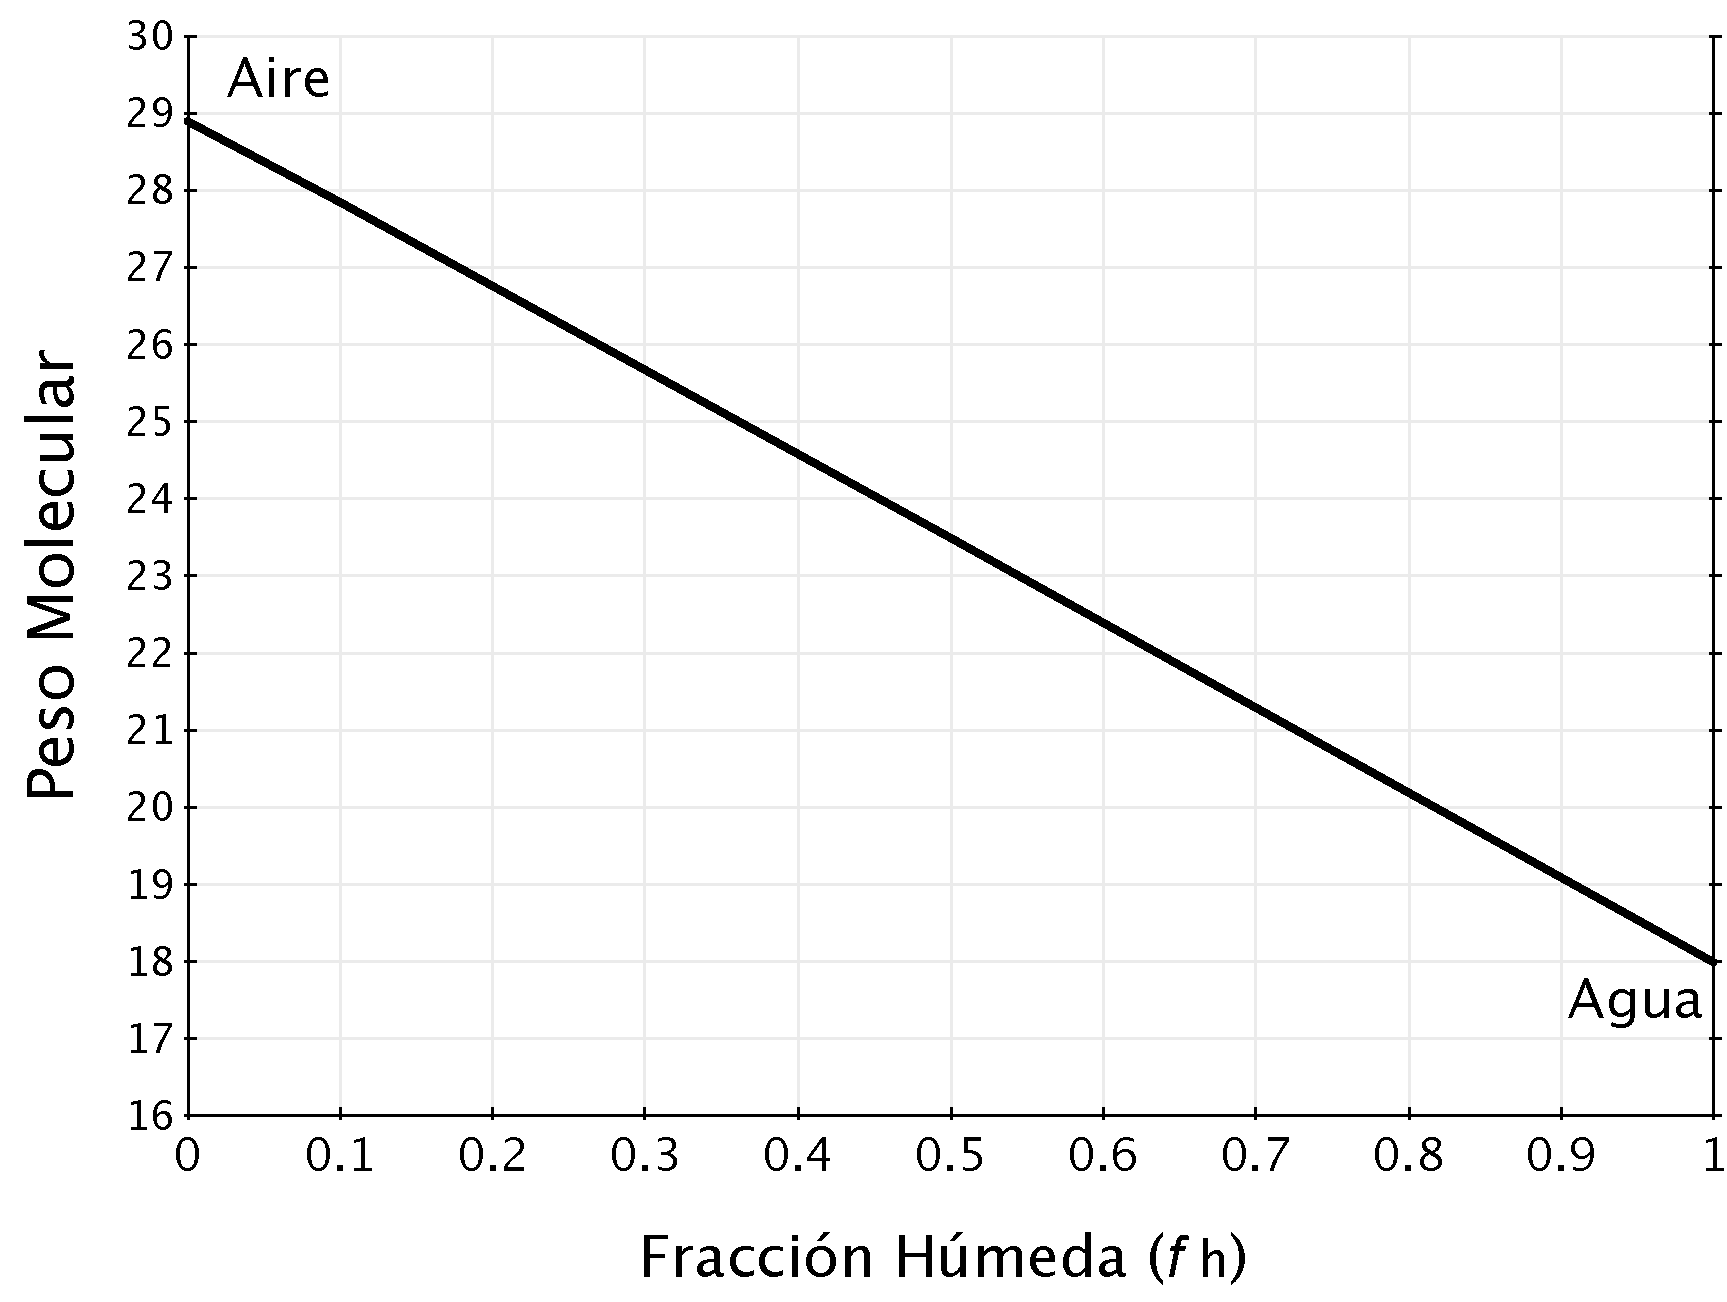
\includegraphics[width=0.70\textwidth]{figuras/FH.pdf}

\caption[Peso molecular aire-agua]{Cambio de la masa molecular promedio de la parcela con respecto a  la fracci\'on h\'umeda$f_H$ }
\label{fig_fh}
\end{center}
\end{figure}

\subsection{Flotaci\'on de una parcela con humedad}

La fuerza con la que es atra\'{\i}da por la gravedad una parcela de aire se puede estimar mediante:
\begin{equation}
F=V\rho g
\label{flot}
\end{equation}
Donde $V$ -- es el volumen, \gloss[word]{densidad} -- es la densidad del aire y $g$  --  es la aceleraci\'on de la gravedad. Substituyendo la  ecuaci\'on~\ref{dens} y ~\ref{pmh} en la ecuaci\'on~\ref{flot} tenemos:
\begin{equation}
F=\left[  (1-f_H)M_a + f_H M_{\ce{H2O}}\right] \frac{\textrm{PV}}{\textrm{RT}}g
\label{fb}
\end{equation}

\begin{figure}[htbp]
\begin{center}
\setlength{\unitlength}{1mm}
\begin{picture}(50,40)
\put (5,5){\line(2,1){7}} %Linea inf derecha
\put(12,8.5){\line(1,0){20}}% linea inf de atras
\put(12,8.5){\line(0,1){25}}
\thicklines
\put(5,30){\line(1,0){20}\line(2,1){7}} %Lineas superiores
\put(5,30){\line(2,1){7}}
\put(12,33.5){\line(1,0){20}} 
\put (5,5){\line(1,0){20}\line(2,1){7}} % Lineas Inferiores
\multiput(5,5)(20,0){2}{\line(0,1){25}}
\put(32,8.5){\line(0,1){25}}
% Flecha y texto izquierdo
%\put(3,19){\vector(0,1){11}}
%\put(3,15){\vector(0,-1){10}} % Flecha abajo
%\put(0,16){$dz$}
% Parte derecha
%\put(34,8){{\footnotesize $z$}}
%\put(34,19){{\footnotesize $\rho$}}
\put(14,16){{\footnotesize $F_g$}}
\put(18,15){\vector(0,-1){6}}
\put(19,22){{\footnotesize $F_b$}}
\put(18,21){\vector(0,1){6}}
%\put(34,32){\footnotesize $z+dz$}
% Parte inferior
%\put(9,1){{\scriptsize $P_b A$}}
%\put(16,0){\vector(0,1){5}}
\end{picture}
\caption{Fuerzas en una parcela de flotaci\'on ($F_b$) y atracci\'on por la gravedad ($F_g$).}
\label{fig_flo1t}
\end{center}
\end{figure}
El principio de Arqu\'{\i}medes nos dice que la fuerza de flotaci\'on ($F_b$) es igual al volumen desplazado, considerando que se desplaza aire seco ($f_H=0$), como se observa en la Figura~\ref{fig_flo1t}, entonces la ecuaci\'on~\ref{fb} quedar\'{\i}a: 
\begin{equation}
F_b=  M_a  \frac{\textrm{PV}}{\textrm{RT}}g
\label{fb1}
\end{equation}

Por otra parte la parcela con humedad ($f_H>0$) es atra\'{\i}da por la fuerza de gravedad ($F_g$) y ser\'{\i}a igual a:

\begin{equation}
F_g=\left[  (1-f_H)M_a + f_H M_{\ce{H2O}}\right] \frac{\textrm{PV}}{\textrm{RT}}g
\label{fg}
\end{equation}

Para las mismas condiciones de presi\'on (P) y temperatura (T),  y observando que el t\'ermino $M_a$ es mayor que $[(1-f_H)M_a + f_H M_{\ce{H2O}}]$ nos indica que $F_b$ es mayor que la fuerza de atracci\'on de la gravedad $F_g$, haciendo que la parcela con humedad, rodeada de aire seco, posea una resultante ascendente.

\subsection{Aceleraci\'on de una parcela con humedad}
Se puede estimar la aceleraci\'on de una parcela inestable, de ah\'{\i} se puede estimar la velocidad en un tiempo dado. La aceleraci\'on (a) ascendente se le conoce como flotaci\'on (B).
\begin{figure}[htbp]
\begin{center}
\setlength{\unitlength}{1mm}
\begin{picture}(50,40)
\put (5,5){\line(2,1){7}} %Linea inf derecha
\put(12,8.5){\line(1,0){20}}% linea inf de atras
\put(12,8.5){\line(0,1){25}}
\thicklines
\put(5,30){\line(1,0){20}\line(2,1){7}} %Lineas superiores
\put(5,30){\line(2,1){7}}
\put(12,33.5){\line(1,0){20}} 
\put (5,5){\line(1,0){20}\line(2,1){7}} % Lineas Inferiores
\multiput(5,5)(20,0){2}{\line(0,1){25}}
\put(32,8.5){\line(0,1){25}}
% Flecha y texto izquierdo
\put(3,19){\vector(0,1){11}}
\put(3,15){\vector(0,-1){10}} % Flecha abajo
\put(0,16){$\mathrm{d}z$}
% Parte derecha
\put(34,8){{\footnotesize $z$}}
\put(13,15){{\footnotesize $\rho'gA\,\mathrm{d}z$}}
\put(34,19){{\footnotesize $\rho$}}
\put(16,13){\vector(0,-1){6}}
\put(17,35){{\footnotesize $P_s A$}}
\put(16,37){\vector(0,-1){6}}
\put(34,32){\footnotesize $z+\mathrm{d}z$}
% Parte inferior
\put(9,1){{\scriptsize $P_b A$}}
\put(16,0){\vector(0,1){5}}
\end{picture}
\caption{Fuerzas en una parcela con densidad diferente a los alrededores}
\label{fig_flot}
\end{center}
\end{figure}

Las fuerzas que act\'uan sobre la parcela, se muestran en la Fig.\ref{fig_flot}, la fuerza de flotaci\'on $F_b$ se representa como la fuerza ascendente ($P_bA$), la fuerza de la columna de aire ($F_s = P_sA$) y el peso de la parcela ($\rho'gA\,\mathrm{d}z$). Las cantidades asociadas a la parcela se identifican con el ap\'ostrofe (') y los par\'ametros ambientales no lo poseen.
\begin{equation}
\sum F= F_b +F_s+F_\textrm{peso} =P_bA-P_sA-\rho'gA\,\mathrm{d}z
\label{balance1}
\end{equation}

Las fuerzas de la ec.~\ref{balance1} no est\'an en equilibrio, as\'{\i} tenemos la necesidad de mantener la aceleraci\'on. Dividiendo ambos lados de la ecuaci\'on por la masa de la parcela ($\rho'V$), y que para el caso de la atm\'osfera terrestre $\mathrm{d}P/\mathrm{d}z= -\rho g$ tenemos:
\begin{equation}
\frac{\sum F}{\rho'V}= \frac{-\frac{P_s-P_b}{dz}-\rho'g}{\rho'}=\frac{-(-\rho g)-\rho'g}{\rho'}
\label{balance2}
\end{equation}
Considerando que se encuentra la parcela de aire a la misma temperatura del aire seco de los alrededores, sabiendo  que $\rho=PM/RT$y que  la aceleraci\'on (a)  $a=F/m$ :
\begin{equation}
a\equiv B=\frac{(\rho -\rho')g}{\rho'}= \frac{(M_a-M_w)g}{M_w}
\label{balance3}
\end{equation}

Sustituyendo la ecuaci\'on~\ref{pmh} en la ecuaci\'on~\ref{balance3} nos da que la aceleraci\'on por flotaci\'on (B) es:
\begin{equation}
B=\frac{(M_a-M_{\ce{H2O}})f_H }{M_a-(M_a-M_{\ce{H2O}})f_H} g
\label{bouyant}
\end{equation}
Al substituir los valores de $M_a$ y $M_{\ce{H2O}}$ , considerando que fuera  vapor de agua exclusivamante ($f_H=1$) la ecuaci\'on~\ref{bouyant} nos indica que la aceleraci\'on m\'axima de una parcela seria de  $6$ \metre/\square\second . La ecuaci\'on anterior nos indica que cualquier parcela que contenga vapor de agua va a ascender.

Para el caso cuando las temperaturas no son iguales,  donde $T_1$ es la temperatura del aire, $T_2$ es de la parcela tenemos:
\begin{equation}
B=\frac{\frac{T_2}{T_1}M_a-M_a+(M_a-M_{\ce{H2O}})f_H }{M_a-(M_a-M_{\ce{H2O}})f_H} g
\label{bouyant2}
\end{equation}
Para el caso de una parcela con humedad y m\'as caliente que los alrededores ($T_2>T_1$) la aceleraci\'on de la flotaci\'on ser\'a mayor que cuando las temperaturas son iguales ($T_2=T_1$). 

\section{Cin\'etica Qu\'{\i}mica}
La cin�tica qu�mica es una rama de la qu�mica que se encarga de estudiar la velocidad de las reacciones qu�micas y los factores que la afectan. Es decir, se ocupa de analizar c�mo cambia la concentraci�n de los reactivos y productos a lo largo del tiempo durante una reacci�n qu�mica.

La velocidad de una reacci�n qu�mica se refiere a la rapidez con la que los reactivos se convierten en productos. Esta velocidad puede ser influenciada por diversos factores, como la concentraci�n de los reactivos, la temperatura, la presi�n, el �rea de superficie de los reactivos, la presencia de catalizadores y la presencia de inhibidores.

La cin�tica qu�mica utiliza experimentos y m�todos matem�ticos para determinar la forma en que la velocidad de una reacci�n var�a con respecto a los cambios en los factores mencionados anteriormente. A partir de estos estudios, se pueden obtener ecuaciones cin�ticas que describen c�mo la concentraci�n de los reactivos y productos cambia en funci�n del tiempo.

Existen diferentes tipos de reacciones qu�micas, y la cin�tica qu�mica permite clasificarlas en reacciones r�pidas o lentas. Adem�s, proporciona informaci�n sobre los mecanismos de reacci�n, que son las etapas o pasos individuales que ocurren durante una reacci�n qu�mica.

La cin�tica qu�mica es de gran importancia en diversas �reas, como la s�ntesis de productos qu�micos, la producci�n de energ�a, la industria farmac�utica y la investigaci�n en ciencias ambientales. Comprender la velocidad de las reacciones qu�micas es fundamental para optimizar los procesos industriales, desarrollar nuevos medicamentos y comprender c�mo los contaminantes afectan al medio ambiente.

En resumen, la cin�tica qu�mica es una rama de la qu�mica que se dedica al estudio de la velocidad de las reacciones qu�micas y los factores que la afectan. A trav�s de experimentos y an�lisis matem�ticos, busca comprender c�mo cambia la concentraci�n de los reactivos y productos a lo largo del tiempo, lo que resulta fundamental para numerosas aplicaciones cient�ficas e industriales.

\section{Velocidades de reacci�n}\index{velocidades@velocidades de reacci�n}
Las velocidades de reacci�n se refieren a la rapidez con la que ocurre una reacci�n qu�mica en particular. Estas velocidades pueden variar ampliamente, desde reacciones muy r�pidas que ocurren en fracciones de segundo hasta reacciones extremadamente lentas que pueden llevar d�as o incluso a�os para completarse.

La velocidad de una reacci�n qu�mica se determina midiendo c�mo cambia la concentraci�n de los reactivos o productos a lo largo del tiempo. Por lo general, se expresa como la cantidad de sustancia que se forma o se consume por unidad de tiempo.

Existen diferentes formas de expresar las velocidades de reacci�n. La m�s com�n es la velocidad promedio, que se calcula dividiendo el cambio en la concentraci�n de un reactivo o producto entre un intervalo de tiempo determinado. Sin embargo, es importante tener en cuenta que la velocidad de una reacci�n puede cambiar a medida que los reactivos se consumen y los productos se forman, por lo que la velocidad instant�nea, que se obtiene en un punto espec�fico de la reacci�n, puede ser diferente a la velocidad promedio.

En resumen, las velocidades de reacci�n se refieren a la rapidez con la que ocurre una reacci�n qu�mica y se determinan mediante la medici�n de los cambios en la concentraci�n de los reactivos o productos a lo largo del tiempo. La fot�lisis es un tipo de reacci�n que implica la descomposici�n de sustancias mediante la absorci�n de energ�a radiante, como la luz. La luz act�a como un agente activador que proporciona la energ�a necesaria para romper los enlaces qu�micos y generar productos diferentes.

La reacciones en la fase gas se pueden clasificar dependiendo del n\'umero de reactivos involucrados as\'{\i} tenemos que las siguientes leyes de velocidad:
\begin{enumerate}
\item Reacciones de primer orden.

Una reacci�n de primer orden es una reacci�n qu�mica en la que la velocidad de reacci�n depende de la concentraci�n de un solo reactivo elevado a la primera potencia. En otras palabras, la velocidad de la reacci�n es directamente proporcional a la concentraci�n del reactivo.
	 \begin{equation*}
	\frac{\mathrm{d}\textrm[A]}{\mathrm{d}t}=-k[\textrm{A}]
	\end{equation*}
Donde $\mathrm{d}[A]/\mathrm{d}t$ representa la velocidad de la reacci�n, $k$ es la constante de velocidad y $[A]$ es la concentraci�n del reactivo $A$. La constante de velocidad $k$ es una constante espec�fica para una reacci�n dada y depende de la naturaleza de la reacci�n y de la temperatura.

La cin�tica de una reacci�n de primer orden implica que la velocidad de reacci�n disminuye a medida que la concentraci�n del reactivo disminuye. Esto se debe a que hay menos mol�culas de reactivo disponibles para reaccionar, lo que reduce las colisiones efectivas y, por lo tanto, disminuye la velocidad de la reacci�n.

Un ejemplo com�n de una reacci�n de primer orden es la descomposici�n radioactiva. En este caso, la concentraci�n de un is�topo radiactivo disminuye con el tiempo debido a su desintegraci�n. La velocidad de desintegraci�n de un is�topo radiactivo es proporcional a la concentraci�n del is�topo presente, y se expresa mediante una constante de velocidad espec�fica para ese is�topo. Otros ejemplos los tenemos con:
 \ce{A -> B +C}\index{reaccion@reacci\'on!unimolecular}
	\begin{description}
		\item[a) Fot\'olisis]  \ce{NO2 + h{\nu} -> NO + O {\cdot}}
		\item[b) T\'ermicas] \ce{CH3COONO3 -> CH3-CO3 + NO2}
	\end{description}
Integrando la ecuaci\'on tenemos:
	\begin{equation*}
	\ln \textrm{A} = -kt
	\end{equation*}
	donde las unidades de $k$ son $s^{-1}$ y de A  son mol�culas/cm$^3$
	
En resumen, una reacci�n de primer orden es aquella en la que la velocidad de reacci�n es directamente proporcional a la concentraci�n de un solo reactivo elevado a la primera potencia. Estas reacciones se describen mediante una expresi�n matem�tica que muestra c�mo la velocidad de reacci�n var�a con la concentraci�n del reactivo. En el caso de una reacci�n atmosf�rica, la descomposici�n del ozono puede considerarse como una reacci�n de primer orden, donde la velocidad de descomposici�n est� determinada principalmente por la concentraci�n de ozono presente en la atm�sfera.

\item Reacciones de Segundo Orden  \ce{A + B -> C + D}\\\index{reaccion@reacci\'on!bimolecular}
Las reacciones de segundo orden son un tipo de reacci�n qu�mica en la cual la velocidad de reacci�n depende de la concentraci�n de dos reactivos diferentes. Es decir, la velocidad de reacci�n es proporcional al producto de las concentraciones de ambos reactivos elevadas a la primera potencia. Matem�ticamente, se representa mediante una ecuaci�n de segundo orden.

En el contexto de la qu�mica atmosf�rica, un ejemplo com�n de una reacci�n de segundo orden es la reacci�n entre los �xidos de nitr�geno (NOx) y el ozono (\ce{O3}). Estos compuestos son precursores de la formaci�n de smog fotoqu�mico y tienen un impacto significativo en la calidad del aire.
\reaction{O3 + NO -> NO2 + O2}
La reacci�n entre los �xidos de nitr�geno y el ozono puede describirse como una reacci�n de segundo orden, donde la velocidad de reacci�n depende de la concentraci�n de ambos reactivos. La ecuaci�n cin�tica general para una reacci�n de segundo orden se expresa de la siguiente manera:
 \begin{equation*}
\ce{Rapidez = - k[NOx][O3]}
 \end{equation*}
Donde ``Rapidez'' representa la velocidad de reacci�n, $k$ es la constante de velocidad y [NOx] y [\ce{O3}] son las concentraciones de los reactivos �xidos de nitr�geno y ozono, respectivamente.

En este caso, la velocidad de reacci�n es proporcional al producto de las concentraciones de �xidos de nitr�geno y ozono. A medida que aumentan las concentraciones de ambos reactivos, la velocidad de reacci�n tambi�n aumenta. Sin embargo, si la concentraci�n de uno de los reactivos disminuye, la velocidad de reacci�n disminuir� en consecuencia.

La reacci�n de segundo orden entre los �xidos de nitr�geno y el ozono es importante en la qu�mica atmosf�rica, ya que contribuye a la formaci�n de oxidantes fotoqu�micos, como el di�xido de nitr�geno (\ce{NO2}), que puede tener efectos adversos en la salud humana y en el  ambiente.

 \begin{equation*}
	-\frac{\mathrm{d}[\textrm{A}]}{\mathrm{d}t}=-\frac{\mathrm{d}[\textrm{B}]}{\mathrm{d}t}=\frac{\mathrm{d}[\textrm{C}]}{\mathrm{d}t}=k[\textrm{A}][\textrm{B}]
	\end{equation*}
	las unidades de k son {\centi\cubic\metre}/{molec$\cdot $\second}
	
En resumen, las reacciones de segundo orden son aquellas en las que la velocidad de reacci�n depende de la concentraci�n de dos reactivos diferentes. En el caso de la qu�mica atmosf�rica, un ejemplo de una reacci�n de segundo orden es la reacci�n entre los �xidos de nitr�geno y el ozono. La velocidad de reacci�n est� determinada por el producto de las concentraciones de ambos reactivos y desempe�a un papel importante en la formaci�n de contaminantes atmosf�ricos como el smog fotoqu�mico.

\item Termoleculares \ce{A + B + C -> D  + E +\ldots}\\\index{reaccion@reacci\'on!termolecular}
Las reacciones termoleculares son un tipo de reacci�n qu�mica en la que tres o m�s mol�culas colisionan y se combinan para formar productos. Estas reacciones son bastante comunes en la qu�mica atmosf�rica y desempe�an un papel importante en la formaci�n y degradaci�n de diferentes compuestos presentes en la atm�sfera.

En el contexto de la qu�mica atmosf�rica, un ejemplo de una reacci�n termolecular es la formaci�n de ozono (O3) a partir del ox�geno molecular (O2). Esta reacci�n ocurre en la estratosfera, donde la radiaci�n ultravioleta proveniente del sol desencadena una serie de procesos fotoqu�micos.

La formaci�n de ozono se puede describir mediante la siguiente reacci�n termolecular:

\reaction{O2 + O2 + M ->  O3 + M}

En esta reacci�n, dos mol�culas de ox�geno (\ce{O2}) colisionan con una mol�cula inerte (representada como M) y se combinan para formar una mol�cula de ozono (\ce{O3}) y otra mol�cula inerte.

Las reacciones termoleculares son m�s comunes en la atm�sfera superior, donde las densidades de mol�culas son m�s bajas y, por lo tanto, las probabilidades de colisiones m�ltiples aumentan. Estas reacciones juegan un papel importante en la qu�mica atmosf�rica, ya que contribuyen a la formaci�n y degradaci�n de diferentes especies qu�micas.

Es importante tener en cuenta que las reacciones termoleculares pueden ser altamente dependientes de la energ�a y la temperatura. La energ�a necesaria para superar la barrera de activaci�n y permitir que las mol�culas colisionen de manera efectiva es proporcionada por la radiaci�n solar en el caso de la atm�sfera terrestre.

En resumen, las reacciones termoleculares en la qu�mica atmosf�rica involucran la colisi�n de tres o m�s mol�culas para formar productos. Un ejemplo destacado es la formaci�n de ozono a partir del ox�geno molecular. Estas reacciones son importantes para comprender los procesos fotoqu�micos y la formaci�n de diferentes compuestos atmosf�ricos en la estratosfera y otras regiones de la atm�sfera.


\reaction{O2 + O + M -> O3 + M}

 \begin{equation*} -\frac{\mathrm{d}[\textrm{A}]}{\mathrm{d}t}=k[\textrm{A}][\textrm{B}][\textrm{C}]
 \end{equation*}
 
 \item Heterog\'eneas (entre fases): Gobernadas por la difusi\'on molecular. La velocidad de colisi\'on del \'atomo B en una superficie por unidad de \'area =$\bar{c}$/4[B]. \index{reaccion@reacci\'on!heterogenea}
\begin{equation*}
-\frac{\mathrm{d}[\textrm{B}]}{\mathrm{d}t}=\frac{\bar{c}}{4}[\textrm{B}]\alpha A
\end{equation*}
 donde $\bar{c}$ es la velocidad molecular promedio \begin{equation}
\bar{c}=\left(\frac{8kT}{\pi M}\right)^{0.5}
\end{equation}
$A$ es el \'area de superficie y $\alpha$ es el coeficiente de adhesi\'on
\end{enumerate}

\section{Tiempo de vida media}\index{vida@vida media}\index{tiempo!de vida media}
Definiremos el tiempo de vida media de un reactivo como el tiempo necesario para que haya reaccionado la mitad de su concentraci�n inicial

En el caso de una reacci�n de primer orden, cuya ecuaci�n de velocidad sabemos que es: 

\begin{equation*}
\nu =k\cdot [A]
\end{equation*}

Entonces, seg�n la definici�n de  $t_{1/2}$ , tenemos que:

\begin{equation*}
t=t_{1/2} \Longrightarrow  [A]=\frac{[A]_0}{2}
\end{equation*}

Usando la f�rmula logar�tmica para las reacciones de primer orden:
\begin{equation*}
\ln[A]=\ln[A]_0-k\cdot t
\end{equation*}
tendremos que: 

$$\ln\frac{[A]_0}{2}=\ln[A]_0-k\cdot t_{1/2}$$

por lo que:

$$\ln[A]_0-\ln2-\ln[A]_0=-k\cdot t_{1/2}$$

y nos queda que:

$$t_{1/2}=\frac{-\ln2}{-k}=\frac{\ln2}{k}$$

De esta expresi�n, vemos que el tiempo de vida media es, en este caso, independiente de la concentraci�n inicial. Por otra parte, se evidencia que la constante de velocidad espec�fica tiene dimensiones de tiempo$^{-1}$y tambi�n es independiente de la concentraci�n inicial.

\section{Tiempo de residencia}\index{tiempo!de residencia}
Los productos qu�micos se inyectan continuamente en la atm�sfera desde fuentes naturales y antr�picas\index{antr�pica}, y tambi�n se producen por reacciones qu�micas en el aire. Sin embargo, la composici�n qu�mica general de la atm�sfera no cambia mucho en per�odos de tiempo relativamente cortos (aunque, como veremos, hay excepciones importantes). Esto se debe a que existen sumideros que eliminan trazas de sustancias qu�micas de la atm�sfera aproximadamente a la misma velocidad con la que se inyectan (y/o se producen dentro) de la atm�sfera, de modo que la mayor�a de las sustancias qu�micas en el aire existen en condiciones m�s o menos estables.s

Un par�metro importante relacionado con una sustancia qu�mica en condiciones de estado estacionario es su tiempo de residencia o vida �til (\gloss[word]{tresid}) en la atm�sfera, que se define como:
\begin{equation*}
\tau=\frac{M}{F}
\end{equation*}
donde $M$ es la cantidad de sustancia qu�mica en la atm�sfera y $F$ la salida (es decir, tasa de eliminaci�n m�s tasa de destrucci�n) de la sustancia qu�mica de la atm�sfera. Si $M$ y $F$ cambian con el tiempo
\begin{equation*}
\tau_t=\frac{M_t}{F_t}
\end{equation*}
donde el sub�ndice $t$ indica el valor en el momento t. Podemos definir, de manera an�loga, el tiempo de residencia en t�rminos del influjo (es decir, tasa de entrada m�s tasa de producci�n) de una sustancia qu�mica a la atm�sfera.

\begin{table}[!hb]
\caption{Tiempo de residencia de gases atmosf�ricos}
\begin{center}
\begin{small}
\begin{tabular}{|l|c|}\hline
\textbf{Gas}                           &\textbf{Tiempo de residencia} \\ \hline
Nitr�geno (\ce{N2})              &  $1.6\times10^7$ a \\
Ox�geno (\ce{O2})	            &3,000 -- 10,000 a \\
Di�xido de Carbono  (\ce{CO2})& 3 -- 4 a \\
Metano (\ce{CH4})                &    9 a  \\
Ozono	 (\ce{O3})              &      100 dia \\
Mon�xido de carbono (CO)   &     $\sim  60$ dia \\
Formaldeh�do	 (\ce{CHOH})& 5 -- 10 dia \\
Di�xido de Nitr�geno (\ce{NO2})&0.5 -- 2 dia\\ \hline
\end{tabular}
\end{small}
\end{center}
\label{tresidencia}
\end{table}%

\begin{figure}[htbp]
\begin{center}
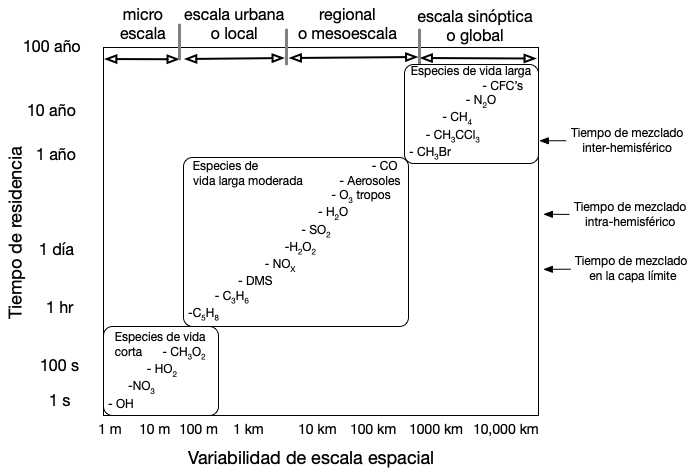
\includegraphics[width=0.95\textwidth]{figuras/tiempo_residencia.png}

\caption[Tiempos de residencia]{Tiempos de residencia de gases en la atm�sfera.}
\label{fig_tresidencia}
\end{center}
\end{figure}
Si una especie qu�mica tiene un tiempo de residencia muy corto (o muy largo) en la atm�sfera, generalmente se producir�n variaciones significativas en la concentraci�n de la especie en escalas espaciales muy cortas (o muy grandes) (Fig.~\ref{fig_tresidencia}). Las especies con tiempos de residencia cortos estar�n presentes en altas concentraciones cerca de fuentes localizadas y en bajas concentraciones muy alejadas de sus fuentes.

\section{Fotoqu\'{\i}mica}\index{fotoquimica@fotoqu\'{\i}mica}

La contaminaci\'on en las ciudades se da principalmente por la conversi\'on de los contaminantes primarios a contaminantes secundarios mediante la interacci\'on con la luz solar. Estos contaminantes se caracterizan principalmente por su alto nivel de oxidaci\'on que afectan los materiales, plantas e irritan ojos y garganta. As\'{\i}mismo influyen en la disminuci\'on de la visibilidad y generaci\'on de olores.

No toda la luz participa en las reacciones, s\'olo la luz que es absorbida puede producir un cambio fotoqu\'{\i}mico, as\'{\i} tenemos que dependiendo de la longitud de onda (\gloss[word]{londa}) se pueden producir un efecto
\begin{enumerate}
\item El lejano IR, microondas influyen en la rotaci\'on de las mol\'eculas.\index{microondas}
\item El infrarrojo en la vibraci\'on
\item La luz visible y ultravioleta en niveles de electrones.
\end{enumerate}

La fotodisociaci\'on\index{fotodisociacion@fotodisociaci\'on} es un proceso en dos pasos el primero la absorci\'on de un fot\'on ($h\nu$)\index{foton@fot\'on} (donde  \gloss[word]{hplank}  es la contante de Planck)\index{constante!Planck} que conduce a un estado exitado.

 \begin{equation*}
\ce{A + h{\nu}    -> A^* } \end{equation*}
posteriormente se produce la disociaci\'on de A$^*$ en dos productos tales como:
\reaction*{A^* -> B + C}
 

\section{Visibilidad}\index{visibilidad}

La visibilidad se reduce por la absorci\'on y esparcimiento\index{esparcimiento} de la luz en materiales l\'{\i}quidos y s\'olidos arrastrados por el aire. La luz visible posee una longitud de onda de $0.38$ a  $0.70\micro\metre$. Part\'{\i}culas en la atm\'osfera con este tama\~no pueden esparcir la luz y con ello causar una reducci\'on en la visibilidad. Esto se puede notar en distancias cortas con altas concentraciones o en grandes distancia con bajas concentraciones\footnote{Nota sobre  part\'{\i}culas:  Cuando se especific\'o la norma de part\'{\i}culas, \'estas se regularon como Part\'{\i}culas Suspendidas Totales (PST)\index{PST}. Esta fue la medida de las part\'{\i}culas  en el aire. 
En 1987 en EU la norma cambi\'o a PM$_{10} $-- toda part\'{\i}cula menor a $10\micro\metre$  en di\'ametro.
En 1997, otra norma de  part\'{\i}culas se adicion\'o --- PM$_{2.5}$ -- toda  part\'{\i}cula menor a $2.5\micro\metre$ en di\'ametro.}.

La visibilidad se reduce por absorci\'on y esparcimiento de la luz de  materiales l\'{\i}quido y s\'olidos arrastrados por el aire. Los gases que afectan la visibilidad en el aire son el bi\'oxido de azufre (\ce{SO2}), el mon\'oxido de nitr\'ogeno (NO) y el vapor de agua. (\ce{H2O}). En el aire limpio se puede ver hasta una distancia de 150 millas y el humo llega a reducir la visibilidad de 1 a 3 millas. Una concentraci\'on de 2,000 part/cm$^3$ se polvo puede ocultar monta\~nas y 100,000 part/cm$^3$ reducen la visibilidad a 1 milla. Concentraciones de \ce{NO2} de 8 a 10 ppm reducen la visibilidad a 1 milla.

Consid\'erese un objeto iluminado por un rayo de intensidad ($I$), a una distancia $x$ del observador
\begin{equation}
\mathrm{d}I=-\sigma I\, \mathrm{d}x
\end{equation}
donde \gloss[word]{extincion} es el coeficiente de extinci\'on,\index{coeficiente!extincion@extinci\'on} $\mathrm{d}x$ es la distancia recorrida, $\mathrm{d}I$ es la reducci\'on de la intensidad por la absorci\'on y dispersi\'on e $I_0$ es la intensidad inicial. Integrando desde 0 a $d$ tenemos
\begin{equation}
I =I_0 e^{-\sigma d}
\end{equation}
$\sigma$ incluye efectos de absorci\'on y dispersi\'on de mol\'eculas de gas y aerosoles.

\begin{equation}
I =I_0 e^{-(a+s)d}
\end{equation}
donde $a$ es el coeficiente de absorci\'on y $s$ es el coeficiente de esparcimiento.

La atenuaci\'on de la luz producida en la atm\'osfera por dipesi\'on se deben a par\'{\i}culas de tama\~no comparable a la longitud de onda (\gloss[word]{londa}) de la luz incidente. Esto es el esparcimiento de \gloss[Word]{mie}\index{Mie@\textbf{Mie}!esparcimiento} y es el fen\'omeno responsable de la reducci\'on de la visibilidad. En el esparcimiento de Mie, se genera m\'as esparcimiento hacia delante que en cualquier otra direcci\'on. Al aumentar el tama\~no de la part\'{\i}cula, el esparcimiento hacia delante tambi\'en aumenta.


La f\'ormula de dispersi\'on de Mie (S) es la siguiente:
\begin{equation}
S=NK\pi r^2
\end{equation}
$N$ n\'umero de part\'iculas de radio $r$ por unidad de volumen. $K$ relaci\'on de \'area de dispersi\'on sobre \'area de part\'{\i}cula.

La longitud de onda de la luz del Sol se encuentra entre 0.4 a 0.8\micro\metre\,  con un m\'aximo a 0.52\micro\metre\, por lo que part\'{\i}culas de 0.1 a 1{\micro\metre} son responsables de la disminuci\'on de la visibilidad. Part\'{\i}culas de tama\~no similar invaden los pulmones y afectan a la salud.

\newpage
\begin{exercises}
Conteste con verdadero o falso, o complete las siguientes preguntas:

\exer Todas las reacciones qu\'{\i}micas ocurren  a  la misma velocidad\dotfill (\hskip.12in)\\
\exer La velocidad qu\'{\i}mica se define como el tiempo que tardan los productos en convertirse en reactivos.\dotfill(\hskip.12in)\\
\exer La teor\'{\i}a de las colisiones dice que todas las colisiones producen reacci\'on.\dotfill(\hskip.12in)\\
\exer Especie intermedia que s\'olo existe durante una fracci\'on de segundo y puede dar lugar a los productos o a reactivos es el complejo activado.\dotfill(\hskip.12in)\\
\exer Barrera de energ\'{\i}a que separa el estado de los reactivos y el estado de los produc\-tos es la energ\'{\i}a de activaci\'on \dotfill (\hskip.12in)
\exer Una neutralizaci\'on es aquella reacci\'on en donde se combina un \'acido con una base\dotfill (\hskip.12in)
\exer Escriba las expresiones de las constantes de equilibrio (kc) para las siguientes reacciones:
\subexer \ce{N2 + 3H2(g) ->  2NH3(g)}
\subexer \ce{N2O + 1/2O2 -> 2NO}
\subexer \ce{4NH3 + 3O2 -> 2N2 + 6H2O}
\subexer \ce{H2 + I2 -> 2HI}
\exer Si la constante de equilibrio $Kc$ para la reacci\'on\\ \vskip 3pt \ce{A(g) + 2B(g) <=> G(g)+ 3H(g)} es 2.1$\times10^{-3}$,\\ \vskip 3pt ?`Qu\'e concentraci\'on de H(g) se tiene en el equilibrio con 0.1 M de A(g), 0.25 de B(g) y 0.02M de G(g)
\exer Si la constante de equilibrio (kp)  para la reacci\'on\\\vskip 3pt\ce{2SO2(g) + O2(g) <=> 2SO3(g)} a 820$^\circ$C es 5.18. \\\vskip 3pt?`Cu\'al es la presi\'on parcial de \ce{SO3(g)} que estar\'{\i}a en equilibrio con 0.25 atm de \ce{SO2(g)} y 0.705 atm de \ce{O2(g)}
\exer Mencione tres factores que influyen en la velocidad de reacci\'on.\\
:\hrulefill ,\hrulefill y \hrulefill .
\exer  ?`C\'omo debe ser el valor de la constante de equilibrio ( $K_{eq}$ ) con respecto al uno para que el equilibrio se desplace hacia los productos?\hrulefill
\exer Si un sistema en equilibrio sufre una alteraci\'on el sistema responder\'a de tal forma que compense dicha alteraci\'on es el principio de:\hrulefill
\exer Una soluci\'on de un \'acido y su base conjugada forman una soluci\'on tam\-p\'on o Buffer\dotfill(\hskip.12in)\\
\exer Un \'acido es un donador de :\hrulefill
\exer En la siguiente reacci\'on se\~nale qu\'e compuestos se comportan como \'acido y cu\'ales como base \ce{HCl + H2O ->  H3O^+ + Cl^-}
\exer Un compuesto que puede reaccionar tanto como \'acido o como base se le conoce como:\hrulefill
\exer Llene los espacios en blanco:\\
\begin{tabular}{l|c|c|c|c}
Sustancia & $[H^+]$ & $pH$ & $pOH$ & [OH]\\ \hline
Leche de vaca &    & $6.6$ &$7.4$ &  \\
\hline Jugo de lim\'on & &$2$ & &$1\times10^{-12}$ \\
\hline 
\end{tabular}
\exer A partir de la siguiente reacci\'on:\\\vskip 3pt \ce{2HNO3 + Mg(OH)2 <=> Mg(NO3)2 + 2H2O}\\ \vskip 3pt ?`Qu\'e cantidad de \'acido n\'{\i}trico \ce{(HNO3)} puede reaccionar con 200 g de hidr\'oxido de magnesio \ce{(Mg(OH)2)}. 

\exer ?`Qu\'e significa la $p$ en el t\'ermino de $pH$:
\hrulefill
\end{exercises}

%\begin{chapreferences}{Fisicoquimica de la Atmosfera}
%\bibitem[Cas86]{castellan}
%Gilbert~W. Castellan.
%\newblock {\em Fisicoqu\'{\i}mica}.
%\newblock Fondo de Educativo Interamericano, M\'exico, D.F., 1986.
%
%\bibitem[MP84]{maron}
%Samuel~H. Maron and Carl~F. Prutton.
%\newblock {\em Fundamentos de Fisicoqu\'{\i}mica}.
%\newblock Editorial LIMUSA, {M\'exico, D.F.}, 1984.
%\newblock decimocuarta reimpresi\'on.
% \end{chapreferences}

%\cite{burton}\cite{castellan}\cite{Hein} \cite{maron}\cite{wingrove}
}
{\backmatter

\pagestyle{fancy}

\rhead[\textbf{Glosario}]{\bfseries\thepage}

\printgloss{glsbase,fqba}

\bibliography{bibliografia}

\rhead[\textbf{\'INDICE DE MATERIAS}]{\bfseries\thepage}
\printindex

}

 \end{document} 